%%%%%%%%%%%%%%%%%%%%%%%%%%%%%%%%%%%%%%%%%%%%%%%%%%%%%%%%%%%%%%%%%%%%%%%%%%%%%%%%
% M5P01 (RMP) Real-Time Operating System -- Chinese User Manual
%
% Build with XeLaTeX:
%   latexmk -xelatex -outdir=Build rmp-manual.tex
%
% Seven-chapter R6T1 organisation.
%%%%%%%%%%%%%%%%%%%%%%%%%%%%%%%%%%%%%%%%%%%%%%%%%%%%%%%%%%%%%%%%%%%%%%%%%%%%%%%%
\documentclass[10pt,a4paper,twoside,openany]{book}
\usepackage{rmp-style}

\begin{document}

\frontmatter
\begin{titlepage}
\thispagestyle{empty}
\centering

\vspace*{1.6cm}


\includegraphics[width=2.9cm]{Figure/logo.png}

\vspace{0.55cm}
{\sffamily\small\color{rmpmid}PROKARON\par}

\vfill

{\sffamily\fontsize{28}{34}\selectfont\color{rmppurple}
M5P01（Prokaron）R6T1\\[3pt]
轻量级实时操作系统（六版一型）\par}

\vspace{1.1em}
{\sffamily\fontsize{21}{25}\selectfont\color{rmpgray}技术参考手册\par}

\vspace{1.4em}
{\rmfamily\large\color{rmpmid}
版本 R6T1\quad$\cdot$\quad 二〇二四年六月\par}

\vfill

{\sffamily\small\color{rmpmid}
EDI-Systems\quad$\cdot$\quad \texttt{www.rtospro.com}\par}
\vspace*{1.4cm}

\end{titlepage}

\chapter*{系统特性}
\addcontentsline{toc}{chapter}{系统特性}
\markboth{系统特性}{}

\begin{center}
{\sffamily\large\color{rmpgray}M5P01（Prokaron）R6T1}\\[2pt]
{\sffamily\Large\bfseries\color{rmpgray}轻量级实时操作系统（六版一型）}\\[4pt]
{\rmfamily\color{rmpmid}技术参考手册}\\[12pt]
\end{center}

\begin{description}[leftmargin=0pt,labelindent=0pt,style=nextline,itemsep=8pt]
    \item[\textsf{\color{rmppurple}高易用性}]
    以轻量易用为第一准绳构建的实时操作系统。
    容易配置开发环境及工程路径。
    提供最常见的线程通信接口。

    \item[\textsf{\color{rmppurple}高实时性}]
    强实时策略的全抢占式内核。
    相同优先级的线程之间时间片轮转式调度。
    所有关键操作时间复杂度 O(1)。

    \item[\textsf{\color{rmppurple}高可移植性}]
    在所有实时系统中底层汇编语言数量最少。
    严格按照 ANSI C89 和 MISRA C 要求进行编写，保证对编译器的兼容性。
    最小系统对资源的要求极低。
    可作为客户操作系统运行在其他操作系统上。

    \item[\textsf{\color{rmppurple}高执行效率}]
    对代码关键性能部分进行调优。
    极短的线程切换时间和中断响应时间。

    \item[\textsf{\color{rmppurple}高可靠性}]
    提供参数检查（Assert）功能，进行广泛存在的接口参数检查。
    经形式化验证，相当于 IEC 61508 SIL 4。\footnote{暂时未完成，目前相当于 SIL 2 预认证级别。}
\end{description}

\newcommand{\RMPRevisionHistory}{%
\chapter*{版本历史}
\addcontentsline{toc}{chapter}{版本历史}
\markboth{版本历史}{}

\begin{table}[htbp]
    \centering
    \renewcommand{\arraystretch}{1.25}
    \small
    \begin{tabularx}{\textwidth}{@{}>{\sffamily\bfseries\color{rmppurple}}m{1.8cm}
                                  >{\raggedright\arraybackslash}m{3.2cm}X@{}}
    \toprule
    版本 & 日期（年-月-日） & 说明 \\
    \midrule
    R1T1 & 2018-02-15 & 初始发布。 \\
    R2T1 & 2018-03-12 & 增加了移植说明和附录。 \\
    R4T3 & 2018-07-31 & 修正手册的错误。 \\
    R4T3 & 2018-09-01 & 更新手册到新版本。 \\
    R4T4 & 2018-10-10 & 解除内存管理单元的 128\,MB 限制，使用更优化的圆角矩形绘制算法。 \\
    R4T5 & 2018-11-25 & 解除最大优先级个数的限制，允许更激进的内存用量优化策略。 \\
    R5T1 & 2020-03-01 & 在基本接口之外增加额外的线程通信接口。 \\
    R5T2 & 2023-05-07 & 为信号量增加广播和同步解锁模式。 \\
    R6T1 & 2024-06-26 & 调整钩子宏的位置和声明，调整 GUI 的配置宏规则。 \\
    \bottomrule
    \end{tabularx}
\end{table}
}


\tableofcontents
\clearpage
\phantomsection
\addcontentsline{toc}{chapter}{表目录}
\listoftables
\clearpage
\phantomsection
\addcontentsline{toc}{chapter}{图目录}
\listoffigures
\clearpage
\RMPRevisionHistory

\mainmatter
\chapter{概述}\label{ch:overview}

\section{简介}\label{sec:introduction}

在小型物联网系统中，16到32位的单片机的使用越发普遍。同时，对于开发周期和可靠性的要求也在增长。因此，有必要开发轻量级的小型系统以实现简单高效的物联网应用。同时，在现代系统中，轻量级虚拟化功能的重要性逐渐增加，因此我们也需要一个轻型操作系统来作为其他操作系统的客户机使用。此外，对于此类操作系统，由于缺乏内存保护单元的介入，因此需要进行形式化验证来保证其可靠性。

实时操作系统是一种简单高效易用的全抢占式实时操作系统（Real-Time
Operating
System，RTOS）。它提供了典型RTOS内核所提供的所有特性：全抢占静态优先级时间片轮转调度器，简单的存储管理功能，简明的通信机制以及针对硬件的特殊优化能力。操作系统被设计为可以在仅具2kB
ROM、1kB RAM的微控制器上高效地运行。

本手册从用户的角度提供了的内核API的描述。在本手册中，我们先简要回顾关于小型实时操作系统的若干概念，然后分章节介绍的特性和API。

\subsection{\texorpdfstring{\textbf{设计目的和指标}}{设计目的和指标}}\label{subsec:design-goals-and-specifications}

操作系统的设计目的是创造一个简单易用的开源RTOS内核。这个内核要具有同级别中最好的实时性和可靠性，并且在平均执行效率上和主流内核相近。

\subsection{\texorpdfstring{\textbf{软件版权与许可证}}{软件版权与许可证}}\label{subsec:copyright-and-license}

综合考虑到不同应用对开源系统的不同要求，内核本身所采用的许可证为Unlicensed，但是对一些特殊情况\footnote{比如安防器材和医疗器材等}使用特殊的规定。这些特殊规定是就事论事的，对于每一种可能情况的具体条款都会有不同。

\subsection{易混术语表}\label{subsec:terms-and-definitions}

在本手册中，容易混淆的基本术语规定如下：

\subsubsection{操作系统}\label{subsubsec:operating-system}

指运行在设备上的执行最底层处理器、内存等硬件资源管理的基本软件。

\subsubsection{线程}\label{subsubsec:thread}

线程指操作系统中拥有一个独立执行栈和一个独立指令流的可被调度的实体。一个进程内部可以拥有多个线程，它们共享一个进程地址空间。

\subsubsection{静态分配}\label{subsubsec:static-allocation}

指在系统编译时就决定好资源分配方式的情形。

\subsubsection{动态分配}\label{subsubsec:dynamic-allocation}

指在系统运行过程中，可以更改资源分配的情形。

\subsubsection{软实时}\label{subsubsec:soft-real-time}

指绝大多数情况下操作应该在时限之内完成，但也允许小部分操作偶尔在时限之外完成的实时性保证。

\subsubsection{硬实时}\label{subsubsec:hard-real-time}

指所有操作都必须在时限之内完成的实时性保证。

\subsubsection{常数实时}\label{subsubsec:constant-real-time}

指所有操作对用户输入和系统配置都是O(1)的，而且执行都能在某个有实际意义的常数时限之内完成的实时性保证。这是所有实时保证中最强的一种。

\subsubsection{对某值常数实时}\label{subsubsec:value-constant-real-time}

指所有操作和响应在某值不变的时候都是O(1)的，而且执行都能在某个有实际意义的常数时限之内完成的实时性保证。

\subsection{主要参考系统}\label{subsec:major-reference-systems}

调度器与API部分参考了FreeRTOS（RT Engineering Ltd./Amazon）。

形式化证明参考了seL4（2016 Data61/CSIRO）。

其他各章的参考文献和参考资料在该章列出。

\section{前言}\label{sec:foreword}

操作系统是一种运行在设备上的执行最底层处理器、内存等硬件资源管理的基本软件。对于实时操作系统而言，系统的每个操作都必须是正确的和及时的，其执行时间必须是可预测的。总的而言，有两类实时操作系统：第一类是软实时系统，第二类是硬实时系统。对于软实时系统，只要在大多数时间之内，程序的响应在时限之内即可；对于硬实时系统，系统的响应在任何时候都必须在时限之内。实际上，很少有实时应用或操作系统完全是软实时的或者完全是硬实时的；他们往往是软实时部分和硬实时部分的有机结合。一个最常见的例子是LCD显示屏人机界面部分是软实时的，而电机控制部分是硬实时的。

系统是一种基本实时系统。此类系统是初步展现了实时系统的基本特性的最小系统。它们一般运行在高档8/16位机以及低档32位机上面，需要一个系统定时器。此类系统没有用户态和内核态的区别，但是可以将MMU和MPU配置为保护某段内存。此类系统需要简单的架构相关汇编代码来进行上下文堆栈切换。若要使得其在多种架构上可运行，修改这段汇编代码是必须的。移植往往还涉及系统定时器，堆栈切换，中断管理和协处理器管理。此类系统可以使用定制的链接器脚本也可以不使用，通常而言在涉及到内存保护的时候必须使用定制的链接器脚本。

在此类系统中任务表现为线程。任务函数有可能是可重入的。每个任务会使用单独的执行栈。任务代码和内核代码可以编译在一起也可以不编译在一起。任务调用系统函数往往使用直接的普通函数调用，没有经由软中断进行系统调用的概念。

此类系统具备优先级的概念，并且一般实现了不同优先级之间的抢占和相同优先级之间的时间片轮转调度。此类系统具备初级的内存管理方案，并且这种内存管理方案一般基于SLAB和伙伴系统。

中断对操作系统可以是完全透明的，此时操作系统并不需要知道中断是否已经到来；如果需要在中断中进行上下文切换，那么就必须将堆栈切换汇编插入该中断函数中，此时需要用汇编代码编写中断的进入和退出。

典型的此类操作系统包括RMProkaron、RT-Thread、FreeRTOS、uC/OS、Salvo和ChibiOS。对于此类实时系统，要进行完全的形式化验证通常是容易的，因为内核代码的数量非常少。传统的软件工程最多只能系统性地对软件的功能进行测试，最多能说明软件存在缺陷的可能性很小；而形式化验证可以根据某种规范或者逻辑推演规则，证明系统符合一定的属性，也即相当于证明了在给定条件下系统不可能有缺陷。

\section{实时操作系统及其组件的性能指标}\label{sec:performance-and-specifications-of-rtoses}

当前市场上有几百种不同种类的RTOS存在，而爱好者和个人开发的内核更是数不胜数。这些系统的性能往往是良莠不齐的。我们需要一些指标来衡量这些RTOS的性能。下面所列的指标都只能在处理器架构相同，编译器、编译选项相同的情况下进行直接比较。如果采用了不同的架构、编译器或编译选项，得到的数据没有直接意义，只具有参考性而不具有可比性。一个推荐的方法是使用工业实际标准的ARM或MIPS系列处理器配合GCC -O2选项进行评估。此外，也可以使用Chronos模拟器来进行评估。在评估时还要注意，系统的负载水平可能会对这些值有影响，因此只有在系统的负载水平一致的情况下，这些值才能够被比较。

\subsection{内核大小}\label{subsec:kernel-size}

内核的尺寸是衡量RTOS的一个重要指标。由于RTOS通常被部署在内存极度受限的设备中，因此内核的小体积是非常关键的。内核的尺寸主要从两个方面衡量，一是只读段大小，二是数据段大小。只读段包括了内核的代码段和只读数据段，数据段包括了内核的可读写数据段大小。在基于Flash的微控制器系统中，只读段会消耗Flash，而数据段则会消耗SRAM\hyperref[sec:chapter-bibliography-2]{{[}1{]}}。

由于RTOS是高度可配置的，其内核大小往往不是固定的，而是和所选用的配置紧密相关的。因此，衡量此项性能，应该查看衡量最小内核配置、常见内核配置和最大内核配置下的内核大小\hyperref[sec:chapter-bibliography-2]{{[}1{]}}。

内核大小数据的获得非常简单，只要用编译器编译该内核，然后使用专门的二进制查看器查看目标文件各段的大小即可。

\subsection{执行时间、最坏执行时间及其抖动}\label{subsec:execution-time-worst-case-execution-time-and-jitter}

执行时间指RTOS系统调用的用时大小。最坏执行时间指执行时间在最不利条件下能达到的最大长度。RTOS的最坏执行时间通常会在如下情况下达到：执行最长的系统调用，并在此过程中产生了大量的缓存未命中。RTOS在执行系统调用时一般都会关中断；最坏执行时间通常是系统关中断最长的时间，因此对系统的实时性的影响是非常巨大的。

最坏执行时间可以分成两类：第一类是内核系统调用的最坏执行时间，另一类是线程间同步的最坏执行时间。

要获得第一类最坏执行时间，可以在调用某个系统调用之前，计时器记下此时的时间戳T\textsubscript{s}，然后在系统调用结束之后，再调用计时器记下此时的时间戳T\textsubscript{e}。然后，连续调用两次计时器，记下两个时间戳T\textsubscript{ts}和T\textsubscript{te}，得到调用计时器的额外代价为T\textsubscript{te}-T\textsubscript{ts}。此时，执行时间就是T\textsubscript{e}-T\textsubscript{s}-(T\textsubscript{te}-T\textsubscript{ts})。最坏执行时间就是所有的系统调用测试之中执行时间最大的那一个。

要获得第二类最坏执行时间，可以在通信机制的发送端调用一次计时器，记下此时的时间戳T\textsubscript{s}，在通信机制的接收端调用一次计时器，记下此时的时间戳T\textsubscript{e}。对于调用计时器的代价测量是类似第一类最坏执行时间的。最终得到的T\textsubscript{e}-T\textsubscript{s}-(T\textsubscript{te}-T\textsubscript{ts})就是执行时间。最坏执行时间，就是所有的通信测试之中，执行时间最大的那一个。

执行时间的抖动也是非常重要的。在多次测量同一个系统的执行、通信时间时，我们往往会得到一个分布。这个分布的平均值是平均执行时间，简称执行时间；其标准差\footnote{有时我们也使用极差}被称为执行时间抖动。

对于一个RTOS，我们通常认为执行时间、最坏执行时间和抖动都是越小越好。执行时间又可以详细分成以下几类\hyperref[sec:chapter-bibliography-2]{{[}1{]}}：

\subsubsection{线程切换时间}\label{subsubsec:thread-switch-time}

线程切换时间指从一个线程切换到另外一个线程所消耗的时间。我们用下图的方法进行测量。在测量时，除了使用T\textsubscript{e}-T\textsubscript{s}的方法，也可以使用两次T\textsubscript{s}之间的差值除以2。线程切换包括两种情况，一种情况是同优先级线程之间互相切换，另外一种是由低优先级线程唤醒高优先级线程\hyperref[sec:chapter-bibliography-2]{{[}2{]}}。

在第一种情况下，我们假设图中的两个线程是相同优先级的，而且在测量开始时，我们正执行的是刚刚由线程B切换过来的线程A。

\captionof{table}{线程切换的第一种情况}\label{tab:thread-switch-first-case}

{\def\LTcaptype{none} % do not increment counter
\begin{longtable}[]{@{}
  >{\raggedright\arraybackslash}p{(\linewidth - 2\tabcolsep) * \real{0.4999}}
  >{\raggedright\arraybackslash}p{(\linewidth - 2\tabcolsep) * \real{0.5001}}@{}}
\toprule\noalign{}
\begin{minipage}[b]{\linewidth}\raggedright
线程A
\end{minipage} & \begin{minipage}[b]{\linewidth}\raggedright
线程B
\end{minipage} \\
\midrule\noalign{}
\endhead
\bottomrule\noalign{}
\endlastfoot
永久循环

\{

\textgreater{} 计时T\textsubscript{s}；

切换到线程B；

\} & 永久循环

\{

计时T\textsubscript{e}；

\textgreater{} 切换到线程A；

\} \\
\end{longtable}
}

在第二种情况下，我们假设图中的线程B优先级较高，而且在测量开始时，我们正执行的是刚刚由线程B切换过来的线程A。

\captionof{table}{线程切换的第二种情况}\label{tab:thread-switch-second-case}

{\def\LTcaptype{none} % do not increment counter
\begin{longtable}[]{@{}
  >{\raggedright\arraybackslash}p{(\linewidth - 2\tabcolsep) * \real{0.5000}}
  >{\raggedright\arraybackslash}p{(\linewidth - 2\tabcolsep) * \real{0.5000}}@{}}
\toprule\noalign{}
\begin{minipage}[b]{\linewidth}\raggedright
线程A
\end{minipage} & \begin{minipage}[b]{\linewidth}\raggedright
线程B
\end{minipage} \\
\midrule\noalign{}
\endhead
\bottomrule\noalign{}
\endlastfoot
永久循环

\{

\textgreater{} 计时T\textsubscript{s}；

唤醒B；

\} & 永久循环

\{

计时T\textsubscript{e}；

\textgreater{} 睡眠；

\} \\
\end{longtable}
}

\subsubsection{异步通信时间}\label{subsubsec:asynchronous-communication-time}

异步通信时间指不同线程之间发送和接收异步信号所用的时间。我们用下图的方法进行测量。我们假设线程B已经在接收端阻塞，线程A进行发送，而且线程B的优先级比线程A高\hyperref[sec:chapter-bibliography-2]{{[}2{]}}。

\captionof{table}{线程间异步通信}\label{tab:asynchronous-communication-between-threads}

{\def\LTcaptype{none} % do not increment counter
\begin{longtable}[]{@{}
  >{\raggedright\arraybackslash}p{(\linewidth - 2\tabcolsep) * \real{0.5000}}
  >{\raggedright\arraybackslash}p{(\linewidth - 2\tabcolsep) * \real{0.5000}}@{}}
\toprule\noalign{}
\begin{minipage}[b]{\linewidth}\raggedright
线程A
\end{minipage} & \begin{minipage}[b]{\linewidth}\raggedright
线程B
\end{minipage} \\
\midrule\noalign{}
\endhead
\bottomrule\noalign{}
\endlastfoot
永久循环

\{

\textgreater{} 计时T；

向B线程发送；

\} & 永久循环

\{

计时T\textsubscript{e}；

\textgreater{} 从自己的邮箱接收；

\} \\
\end{longtable}
}

\subsection{中断响应时间、最坏中断响应时间及其抖动}\label{subsec:interrupt-response-time-worst-case-response-time-and-jitter}

中断响应时间指从中断发生到RTOS调用中断对应的处理线程之间的时间。最坏中断响应时间指中断响应时间在最不利条件下能达到的最大长度。最坏中断响应时间通常会在如下情况下达到：在中断处理过程中发生了大量的缓存未命中和快表（Trans
Look-aside
Buffer，TLB）未命中。中断响应时间是RTOS最重要的指标，甚至可以说，RTOS的一切设计都是围绕着该指标进行的。该指标是RTOS对外界刺激响应时间的最直接的标准。

要获得最坏中断响应时间，可以在中断向量的第一行汇编代码\footnote{不能等到函数中再去调用，因为寄存器和堆栈维护也是中断响应时间的一部分}T\textsubscript{e}-T\textsubscript{s}-(T\textsubscript{te}-T\textsubscript{ts})就是中断响应时间。最坏中断响应时间，就是所有的中断响应测试之中，响应时间最大的那一个。

中断响应时间的抖动也是非常重要的。在多次测量同一个系统的中断响应时间时，我们往往会得到一个分布。这个分布的平均值是平均中断响应时间，其标准差\footnote{有时我们也使用极差}被称为中断响应时间抖动。

对于一个RTOS，我们通常认为中断响应时间、最坏中断响应时间和抖动都是越小越好。中断响应时间的测量通常如下所示\hyperref[sec:chapter-bibliography-2]{{[}1{]}{[}3{]}}：

\captionof{table}{中断响应时间}\label{tab:interrupt-response-time}

{\def\LTcaptype{none} % do not increment counter
\begin{longtable}[]{@{}
  >{\raggedright\arraybackslash}p{(\linewidth - 2\tabcolsep) * \real{0.5000}}
  >{\raggedright\arraybackslash}p{(\linewidth - 2\tabcolsep) * \real{0.5000}}@{}}
\toprule\noalign{}
\begin{minipage}[b]{\linewidth}\raggedright
内核
\end{minipage} & \begin{minipage}[b]{\linewidth}\raggedright
线程A
\end{minipage} \\
\midrule\noalign{}
\endhead
\bottomrule\noalign{}
\endlastfoot
硬件中断向量

\{

\textgreater{} 计时T\textsubscript{s}；

从内核向异步端点P发送信号；

\} & 永久循环

\{

计时T\textsubscript{e}；

\textgreater{} 从异步端点P接收信号；

\} \\
\end{longtable}
}

\subsection{实际中断响应时间、最坏实际中断响应时间及其抖动}\label{subsec:realistic-interrupt-response-time-worst-case-and-jitter}

实际中断响应时间指软硬件系统从中断外部信号输入到发出IO操作响应之间的时间。最坏实际中断响应时间指实际中断响应时间在最不利条件下能达到的最大长度。影响实际最坏中断响应时间的因素中，除了那些能影响最坏中断响应时间的因素之外，还有对应的CPU及IO硬件本身的因素。

要获得实际中断响应时间，我们需要一些外部硬件来支持该种测量。比如，我们需要测量某系统的I/O的实际中断响应时间，我们可以将一个FPGA的管脚连接到某CPU或主板的输入管脚，然后将另一个管脚连接到某CPU或者主板上的输出管脚。首先，FPGA向输入管脚发出一个信号，此时FPGA内部的高精度计时器开始工作；在FPGA接收到输出管脚上的信号的时候，FPGA内部的高精度计时器停止工作。最终得到的FPGA内部计时器的时间就是系统的实际中断响应时间。最坏实际中断响应时间，就是所有测试之中，响应时间最大的那一个。

对于一个软硬件系统，我们通常认为实际中断响应时间、最坏实际中断响应时间和抖动都是越小越好。值得注意的是，实际最坏中断响应时间一般会大约等于最坏执行时间加上最坏中断响应时间加上系统CPU/IO的固有延迟。比如，某系统在IO输入来临时刚刚开始执行某系统调用，此时硬件中断向量无法立刻得到执行，必须等到该系统调用执行完毕才可以。等到该系统调用执行完毕时，实际的硬件中断向量才开始执行，切换到处理线程进行处理并产生输出。实际中断响应时间的测量通常如下所示\hyperref[sec:chapter-bibliography-2]{{[}1{]}}：

\captionof{table}{实际中断响应时间}\label{tab:realistic-interrupt-response-time}

{\def\LTcaptype{none} % do not increment counter
\begin{longtable}[]{@{}
  >{\raggedright\arraybackslash}p{(\linewidth - 2\tabcolsep) * \real{0.5000}}
  >{\raggedright\arraybackslash}p{(\linewidth - 2\tabcolsep) * \real{0.5000}}@{}}
\toprule\noalign{}
\begin{minipage}[b]{\linewidth}\raggedright
FPGA（或者示波器）
\end{minipage} & \begin{minipage}[b]{\linewidth}\raggedright
被测系统
\end{minipage} \\
\midrule\noalign{}
\endhead
\bottomrule\noalign{}
\endlastfoot
永久循环

\{

\textgreater{} 发出信号并启动计时器；

接收信号；

停止计时器；

\} & 永久循环

\{

从I/O上接收信号；

最简化的内部处理流程；

从I/O上输出信号；

\} \\
\end{longtable}
}

\section{RMP系统调用格式}\label{sec:rmp-system-call-format}

系统调用是使用系统提供的功能的唯一方法。对于这样的库结构操作系统而言，系统调用和通常的函数调用是一样的。下面是中所有的系统调用接口的列表。

\captionof{table}{RMP系统调用一览}\label{tab:rmp-system-calls}

{\def\LTcaptype{none} % do not increment counter
\begin{longtable}[]{@{}
  >{\raggedright\arraybackslash}p{(\linewidth - 4\tabcolsep) * \real{0.3668}}
  >{\raggedright\arraybackslash}p{(\linewidth - 4\tabcolsep) * \real{0.1076}}
  >{\raggedright\arraybackslash}p{(\linewidth - 4\tabcolsep) * \real{0.5256}}@{}}
\toprule\noalign{}
\begin{minipage}[b]{\linewidth}\raggedright
系统调用名称
\end{minipage} & \begin{minipage}[b]{\linewidth}\raggedright
序号
\end{minipage} & \begin{minipage}[b]{\linewidth}\raggedright
意义
\end{minipage} \\
\midrule\noalign{}
\endhead
\bottomrule\noalign{}
\endlastfoot
RMP\_Thd\_Yield & 0 & 出让当前线程的处理器 \\
RMP\_Thd\_Crt & 1 & 创建一个线程 \\
RMP\_Thd\_Del & 2 & 删除一个线程 \\
RMP\_Thd\_Set & 3 & 设置一个线程的优先级和时间片 \\
RMP\_Thd\_Suspend & 4 & 悬起一个线程 \\
RMP\_Thd\_Resume & 5 & 解除一个线程的悬起 \\
RMP\_Thd\_Delay & 6 & 延时一段时间 \\
RMP\_Thd\_Cancel & 7 & 解除一个线程的延时 \\
RMP\_Thd\_Snd & 8 & 向某线程的邮箱发送数值 \\
RMP\_Thd\_Snd\_ISR & 9 & 从中断向某线程的邮箱发送数值 \\
RMP\_Thd\_Rcv & 10 & 接收本线程邮箱值 \\
RMP\_Sem\_Crt & 11 & 创建一个计数信号量 \\
RMP\_Sem\_Del & 12 & 删除一个计数信号量 \\
RMP\_Sem\_Pend & 13 & 试图获取一个信号量 \\
RMP\_Sem\_Abort & 14 & 解除某线程对信号量的获取 \\
RMP\_Sem\_Post & 15 & 释放信号到某信号量 \\
RMP\_Sem\_Post\_ISR & 16 & 从中断释放信号到某信号量 \\
\end{longtable}
}

\section{本章参考文献}\label{sec:chapter-bibliography}

\protect\phantomsection\label{sec:chapter-bibliography-2}{[}1{]}
T. N. B. Anh and S.-L. Tan, "Real-time operating systems for small
microcontrollers," IEEE micro, vol. 29, 2009.

{[}2{]} R. P. Kar, "Implementing the Rhealstone real-time benchmark,"
Dr. Dobb\textquotesingle s Journal, vol. 15, pp. 46-55, 1990.

{[}3{]} T. J. Boger, Rhealstone benchmarking of FreeRTOS and the Xilinx
Zynq extensible processing platform: Temple University, 2013.

\chapter{系统内核}\label{ch:system-kernel}

\section{系统内核简介}\label{sec:kernel-introduction}

的内核提供了一个可使用的实时操作系统应具有的最简单的功能，主要包括线程、线程延时、邮箱机制和信号量机制。如果用户需要更复杂的机制，那么可以从提供的几种基本机制出发实现其他的机制。本系统还额外提供了一个轻量级图形界面库，它在不使用\footnote{未检测到相关宏被定义}的时候完全不消耗内存。

本系统推荐用于32个优先级以下，64个线程以下的系统。本系统理论上最多支持的线程数量和优先级数量都是无限的，但为了系统效率和易用性，不推荐使用本系统实现超过这个复杂度的嵌入式应用。如果需要实现更复杂的嵌入式应用，推荐使用0等更高级的系统。

\subsection{内核调度器}\label{subsec:kernel-scheduler}

内核的调度器是一个全抢占式的固定优先级时间片轮转的调度器。该类调度器在同一个优先级内部使用时间片轮转法则进行线程调度，在不同的优先级之间则采取抢占式调度策略。和某些RTOS不同，的调度器在某些架构上永远不会关闭中断，从而保证了系统的实时性。为了提高内核的实时性，当处理器具备、等指令时，还可以使用这些指令加速最高优先级查找。

没有\footnote{将来也永远不会}内建对多核系统的直接支持。如果要支持多核处理器也是可能的，这需要编译多个副本并且在每个处理器上运行一个副本，以分区操作系统的方式存在，类似于\hyperref[sec:chapter-bibliography-4]{{[}1{]}}。

\subsection{内存管理与内存保护}\label{subsec:memory-management-and-memory-protection}

提供了一个基于二级分割适配算法（Two-Level Segregated Fit,
TLSF）\hyperref[sec:chapter-bibliography-4]{{[}2{]}{[}3{]}}机制的内存分配器。这个分配器在所有O(1)时间复杂度的内存分配器中具备较高空间效率。然而，在小型嵌入式系统中动态内存分配并不被推荐，因此应该尽量少用该分配器。不具备真正意义上的内存保护功能，各个线程之间的地址是没有隔离的，因此在编写应用程序时应当遵循编程规范。

\subsection{应用升级与应用模块}\label{subsec:application-updating-and-application-modules}

由于本系统相对较为小型，因此不支持应用升级和应用模块。通常而言，使用本系统编译出的完整映像大小不应超过128kB，因此是可以全部升级的。如果需要应用模块功能，那么需要用户自行实现。

\subsection{系统启动流程}\label{subsec:system-boot-sequence}

RMP内核的第一个线程永远是RMP\_Init，它位于内核提供的代码中。RMP\_Init线程负责系统的初期初始化和低功耗，并且它永远不可能停止运行。RMP\_Init线程引出了两个钩子RMP\_Init\_Hook和RMP\_Init\_Idle，它们负责将用户代码导入到内核运行的过程中。关于这两个接口的说明请参见第\ref{subsec:mandatory-hook-interface}节所述。

\section{线程调度接口}\label{sec:thread-scheduling-interface}

由于整个系统都运行在一个地址空间，因此系统仅提供线程抽象。线程可以有就绪、运行、悬起、阻塞\footnote{包括延时、等待信号量、等待邮箱接收、等待邮箱发送四种基本阻塞方式}四种状态，阻塞状态还具有一段时间后接收不到自动返回的功能。悬起状态可以被施加于任何线程，此时该线程总是暂时停止执行，无论其当前处于什么状态。

完整的线程状态转移图如下所示：

\begin{figure}[htbp]
    \centering
    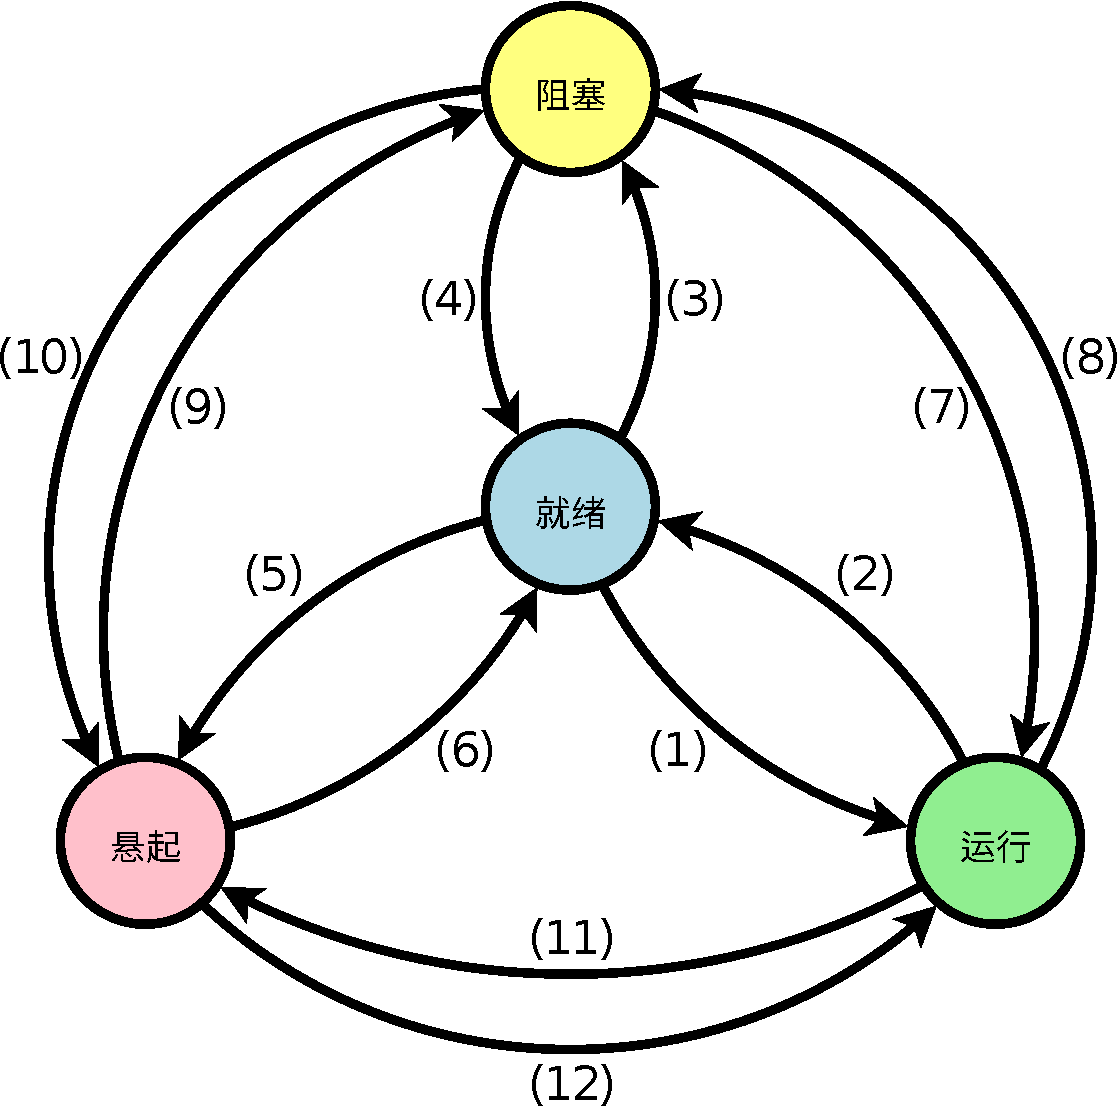
\includegraphics[width=0.72\textwidth]{Figure/thread_state_cn.pdf}
    \caption{线程状态转移图}
    \label{fig:thread-state-transition-diagram}
\end{figure}

图中各个数字标号的意义如下所示：

\captionof{table}{线程状态转移图中各标号的含义}\label{tab:meaning-of-the-labels-in-the-thread-state-transition-diagram}

{\def\LTcaptype{none} % do not increment counter
\begin{longtable}[]{@{}
  >{\raggedright\arraybackslash}p{(\linewidth - 2\tabcolsep) * \real{0.0750}}
  >{\raggedright\arraybackslash}p{(\linewidth - 2\tabcolsep) * \real{0.9250}}@{}}
\toprule\noalign{}
\begin{minipage}[b]{\linewidth}\raggedright
标号
\end{minipage} & \begin{minipage}[b]{\linewidth}\raggedright
代表意义
\end{minipage} \\
\midrule\noalign{}
\endhead
\bottomrule\noalign{}
\endlastfoot
(1) & 该线程处于就绪态且优先级最高，因此由就绪态转入运行态。 \\
(2) & 该线程处于运行态且优先级非最高，因此由运行态转入就绪态。 \\
(3) &
该可能性不存在（图中以虚线表示），线程不可能直接由就绪态进入阻塞态。 \\
(4) &
该线程被解除阻塞且未悬起，且优先级非最高，因此由阻塞态进入就绪态。 \\
(5) & 该线程在就绪态被悬起，因此由就绪态进入悬起态。 \\
(6) &
该线程被解除悬起且未阻塞，且优先级非最高，因此由悬起态进入就绪态。 \\
(7) &
该线程被解除阻塞且未悬起，且优先级最高，因此由阻塞态进入运行态。 \\
(8) & 该线程在邮箱、信号量或延时功能处阻塞，因此由运行态进入阻塞态。 \\
(9) & 该线程在被解除悬起且仍在阻塞，因此由悬起态进入阻塞态。 \\
(10) & 该线程在阻塞态被悬起，因此由阻塞态进入悬起态。 \\
(11) & 该线程在运行态被悬起，因此由运行态进入悬起态。 \\
(12) &
该线程在被解除悬起且未阻塞，且优先级最高，因此由悬起态进入运行态。 \\
\end{longtable}
}

所有的线程调度接口如下表所示：

\captionof{table}{线程调度接口一览}\label{tab:thread-scheduling-interface-summary}

{\def\LTcaptype{none} % do not increment counter
\begin{longtable}[]{@{}
  >{\raggedright\arraybackslash}p{(\linewidth - 6\tabcolsep) * \real{0.3210}}
  >{\raggedright\arraybackslash}p{(\linewidth - 6\tabcolsep) * \real{0.3146}}
  >{\raggedright\arraybackslash}p{(\linewidth - 6\tabcolsep) * \real{0.1759}}
  >{\raggedright\arraybackslash}p{(\linewidth - 6\tabcolsep) * \real{0.1817}}@{}}
\toprule\noalign{}
\begin{minipage}[b]{\linewidth}\raggedright
接口
\end{minipage} & \begin{minipage}[b]{\linewidth}\raggedright
意义
\end{minipage} & \begin{minipage}[b]{\linewidth}\raggedright
锁调度器时调用
\end{minipage} & \begin{minipage}[b]{\linewidth}\raggedright
中断中调用
\end{minipage} \\
\midrule\noalign{}
\endhead
\bottomrule\noalign{}
\endlastfoot
RMP\_Thd\_Crt & 创建线程 & 可 & 不可 \\
RMP\_Thd\_Del & 删除线程 & 可 & 不可 \\
RMP\_Thd\_Set & 设置线程属性 & 可 & 不可 \\
RMP\_Thd\_Yield & 出让处理器 &
不可\footnotemark{} & 不可 \\
RMP\_Thd\_Suspend & 悬起线程 & 不可 & 不可 \\
RMP\_Thd\_Resume & 解除线程悬起 & 可 & 不可 \\
RMP\_Thd\_Delay & 线程延时 & 不可 & 不可 \\
RMP\_Thd\_Cancel & 解除线程延时 & 可 & 不可 \\
RMP\_Thd\_Loop & 线程循环延时 & 可 & 不可 \\
\end{longtable}
}
\footnotetext{不可能阻塞当前线程的操作均可在锁调度器时调用，但可能会阻塞或出让当前线程的操作则不可在锁调度器时调用；这个标准同样适用于后面各章节中列出的接口}

它们可能有如下返回值：

\captionof{table}{线程调度接口的可能返回值}\label{tab:possible-return-values-of-the-thread-scheduling-interface}

{\def\LTcaptype{none} % do not increment counter
\begin{longtable}[]{@{}
  >{\raggedright\arraybackslash}p{(\linewidth - 4\tabcolsep) * \real{0.2741}}
  >{\raggedright\arraybackslash}p{(\linewidth - 4\tabcolsep) * \real{0.0927}}
  >{\raggedright\arraybackslash}p{(\linewidth - 4\tabcolsep) * \real{0.6332}}@{}}
\toprule\noalign{}
\begin{minipage}[b]{\linewidth}\raggedright
返回值
\end{minipage} & \begin{minipage}[b]{\linewidth}\raggedright
数值
\end{minipage} & \begin{minipage}[b]{\linewidth}\raggedright
意义
\end{minipage} \\
\midrule\noalign{}
\endhead
\bottomrule\noalign{}
\endlastfoot
RMP\_ERR\_THD & -1 & 由于线程控制块相关的原因导致操作失败。 \\
RMP\_ERR\_PRIO & -2 & 由于优先级相关的原因导致操作失败。 \\
RMP\_ERR\_SLICE & -3 & 由于时间片相关的原因导致操作失败。 \\
RMP\_ERR\_STACK & -4 & 由于运行栈相关的原因导致操作失败。 \\
RMP\_ERR\_STATE & -5 & 由于线程状态相关的原因导致操作失败。 \\
RMP\_ERR\_OPER & -6 & 由于其他原因导致操作失败。 \\
\end{longtable}
}

具体的各个函数中返回值的意义请在相应函数下查找。

\subsection{创建线程}\label{subsec:create-a-thread}

本操作会创建一个新的线程并使其处于就绪态。新创建的线程总是会被插入到同优先级时间片轮转队列的末尾：如果没有其它干扰，则先创建的线程总是先被调度。

\begin{apidesc}{RMP\_Thd\_Crt}{创建线程}
    \apisig{rmp\_ret\_t RMP\_Thd\_Crt(volatile struct RMP\_Thd* Thread, void* Entry, void* Param, void* Stack, rmp\_ptr\_t Size, rmp\_ptr\_t Prio, rmp\_ptr\_t Slice)}
    \begin{apiparams}
        \apiparam{volatile struct RMP\_Thd* Thread}{指向空的、将被用于该线程的线程控制块的指针。}
        \apiparam{void* Entry}{线程的入口地址。}
        \apiparam{void* Param}{传递给线程的参数。}
        \apiparam{void* Stack}{线程的运行栈的起始地址。如果以数组的形式分配它，则此处填写数组的首地址。某些架构对栈的内存地址有特殊要求\footnote{如必须位于地址空间的低64KiB等；如果涉及堆栈段寄存器，请参见\ref{subsubsec:the-common-memory-model-is-the-small-model}}，此时该地址必须满足这些要求。}
        \apiparam{rmp\_ptr\_t Size}{线程的运行栈的大小，单位为字节。如果以数组的形式分配它，则此处填写数组的大小。}
        \apiparam{rmp\_ptr\_t Prio}{线程的优先级。在本系统中，优先级数字越大，优先级越高。}
        \apiparam{rmp\_ptr\_t Slice}{线程的时间片数量。时间片数量的单位是时钟嘀嗒。}
    \end{apiparams}
    当 \texttt{RMP\_STKSEG\_ENABLE} 非 0 时，\texttt{Param} 与 \texttt{Stack} 之间还有一个 \texttt{rmp\_ptr\_t Segment} 参数，用于指定线程的堆栈段。
    \begin{apiret}
        \apiretval{rmp\_ret\_t}{如果成功，返回0。如果失败则可能有如下返回值：}
        \apiretval{RMP\_ERR\_STACK}{输入的栈区域为0（NULL）或者栈大小放不下上下文。}
        \apiretval{RMP\_ERR\_PRIO}{输入的优先级不小于RMP\_PREEMPT\_PRIO\_NUM。}
        \apiretval{RMP\_ERR\_SLICE}{输入的时间片为0或不小于RMP\_SLICE\_MAX。}
        \apiretval{RMP\_ERR\_THD}{线程控制块为0（NULL）或者正在被使用。}
    \end{apiret}
\end{apidesc}

\subsection{删除线程}\label{subsec:delete-a-thread}

本操作会删除系统中的一个线程。线程被删除后，一切资源将释放，正在向它发送的线程的发送等待将被解除并会返回发送失败。

值得注意的是，的线程并不允许通过返回来直接退出。如果任何一个线程想要终止自己，就必须显式调用这个函数删除自己。这个设计是有意而为，是为了显式地提醒用户线程正被删除，从而方便用户最大限度地避免``创建
- 运行一次 -
删除''的用法\footnote{这种用法应该被``阻塞 - 运行一次 - 再次阻塞''或线程池技术代替}。

\begin{apidesc}{RMP\_Thd\_Del}{删除线程}
    \apisig{rmp\_ret\_t RMP\_Thd\_Del(volatile struct RMP\_Thd* Thread)}
    \begin{apiparams}
        \apiparam{volatile struct RMP\_Thd* Thread}{指向要删除的线程的线程控制块的指针。}
    \end{apiparams}
    \begin{apiret}
        \apiretval{rmp\_ret\_t}{如果成功，返回0。如果失败则可能有如下返回值：}
        \apiretval{RMP\_ERR\_THD}{线程控制块为0（NULL）或者未被使用。}
    \end{apiret}
\end{apidesc}

\subsection{设置线程属性}\label{subsec:set-thread-attributes}

本操作会设置某个线程的时间片和优先级。当只需要设置其中一个时，只要保证另一个参数是RMP\_PREEMPT\_PRIO\_NUM或RMP\_SLICE\_MAX即可。

\begin{apidesc}{RMP\_Thd\_Set}{设置线程属性}
    \apisig{rmp\_ret\_t RMP\_Thd\_Set(volatile struct RMP\_Thd* Thread, rmp\_ptr\_t Prio, rmp\_ptr\_t Slice)}
    \begin{apiparams}
        \apiparam{volatile struct RMP\_Thd* Thread}{指向要更改优先级和时间片的线程的线程控制块的指针。}
        \apiparam{rmp\_ptr\_t Prio}{要设置的优先级。输入RMP\_PREEMPT\_PRIO\_NUM代表不修改优先级。 在本系统中，优先级数字越大，优先级越高。}
        \apiparam{rmp\_ptr\_t Slice}{要设置的时间片数量。输入RMP\_SLICE\_MAX代表不修改时间片。}
    \end{apiparams}
    \begin{apiret}
        \apiretval{rmp\_ret\_t}{如果成功，返回0。如果失败则可能有如下返回值：}
        \apiretval{RMP\_ERR\_PRIO}{输入的优先级大于RMP\_PREEMPT\_PRIO\_NUM。}
        \apiretval{RMP\_ERR\_SLICE}{输入的时间片为0或者大于RMP\_SLICE\_MAX。}
        \apiretval{RMP\_ERR\_THD}{线程控制块为0（NULL）或者未被使用。}
    \end{apiret}
\end{apidesc}

\subsection{出让处理器}\label{subsec:yield-the-processor}

本操作会使当前线程放弃CPU，并且调度器会自动选择下一个线程进行调度。如果当前线程的优先级是最高的，且那个优先级上只有它，那么它仍然会被调度。

\begin{apidesc}{RMP\_Thd\_Yield}{出让处理器}
    \apisig{void RMP\_Thd\_Yield(void)}
    \begin{apiparams}
        \apiparam{无。}{}
    \end{apiparams}
    \begin{apiret}
        \apiretval{无。}{}
    \end{apiret}
\end{apidesc}

\subsection{悬起线程}\label{subsec:suspend-a-thread}

本操作会使某线程悬起，使调度器暂时停止对其的调度。无论线程处于哪个状态，它都可以被悬起，但是已经处于的延时、发送、接收等状态仍继续存在，也即线程处于悬起状态和延时、发送、接收等状态之一的叠加。当延时、发送、接收等状态结束后，如果该线程还处于被悬起状态，那么它将被置于纯粹的悬起状态，仍然不参与调度，直到悬起状态被手动解除。

\begin{apidesc}{RMP\_Thd\_Suspend}{悬起线程}
    \apisig{rmp\_ret\_t RMP\_Thd\_Suspend(volatile struct RMP\_Thd* Thread)}
    \begin{apiparams}
        \apiparam{volatile struct RMP\_Thd* Thread}{指向要悬起执行的线程的线程控制块的指针。}
    \end{apiparams}
    \begin{apiret}
        \apiretval{rmp\_ret\_t}{如果成功，返回0。如果失败则可能有如下返回值：}
        \apiretval{RMP\_ERR\_THD}{线程控制块为0（NULL）或者未被使用。}
        \apiretval{RMP\_ERR\_STATE}{该线程已经被悬起，无法被再次悬起。 该检查即使在关闭时也会执行。}
    \end{apiret}
\end{apidesc}

\subsection{解除线程悬起}\label{subsec:resume-a-suspended-thread}

本操作会解除某个线程的悬起状态，使其有重新参与调度的可能。

\begin{apidesc}{RMP\_Thd\_Resume}{解除线程悬起}
    \apisig{rmp\_ret\_t RMP\_Thd\_Resume(volatile struct RMP\_Thd* Thread)}
    \begin{apiparams}
        \apiparam{volatile struct RMP\_Thd* Thread}{指向要解除悬起的线程的线程控制块的指针。}
    \end{apiparams}
    \begin{apiret}
        \apiretval{rmp\_ret\_t}{如果成功，返回0。如果失败则可能有如下返回值：}
        \apiretval{RMP\_ERR\_THD}{线程控制块为0（NULL）或者未被使用。}
        \apiretval{RMP\_ERR\_STATE}{该线程未被悬起，无法被解除悬起。 该检查即使在关闭时也会执行。}
    \end{apiret}
\end{apidesc}

\subsection{线程延时}\label{subsec:delay-a-thread}

本操作会使当前线程延时一段时间。

\begin{apidesc}{RMP\_Thd\_Delay}{线程延时}
    \apisig{rmp\_ret\_t RMP\_Thd\_Delay(rmp\_ptr\_t Slice)}
    \begin{apiparams}
        \apiparam{rmp\_ptr\_t Slice}{要延时的时间，单位是时间片。}
    \end{apiparams}
    \begin{apiret}
        \apiretval{rmp\_ret\_t}{如果成功，返回0。如果失败则可能有如下返回值：}
        \apiretval{RMP\_ERR\_SLICE}{输入的时间片为0或不小于RMP\_SLICE\_MAX。}
        \apiretval{RMP\_ERR\_OPER}{该延时没有进行完毕就被解除。 该检查即使在关闭时也会执行。}
    \end{apiret}
\end{apidesc}

\subsection{解除线程延时}\label{subsec:cancel-a-thread-delay}

本操作会解除某个线程的延时。

\begin{apidesc}{RMP\_Thd\_Cancel}{解除线程延时}
    \apisig{rmp\_ret\_t RMP\_Thd\_Cancel(volatile struct RMP\_Thd* Thread)}
    \begin{apiparams}
        \apiparam{volatile struct RMP\_Thd* Thread}{指向要解除延时的线程的线程控制块的指针。}
    \end{apiparams}
    \begin{apiret}
        \apiretval{rmp\_ret\_t}{如果成功，返回0。如果失败则可能有如下返回值：}
        \apiretval{RMP\_ERR\_THD}{线程控制块为0（NULL）或者未被使用。}
        \apiretval{RMP\_ERR\_STATE}{该线程未处于延时状态，无法被解除延时。 该检查即使在关闭时也会执行。}
    \end{apiret}
\end{apidesc}

\subsection{线程循环延时}\label{subsec:thread-busy-wait}

本操作会使当前线程陷入死循环一段时间。与其它线程接口不同，它可以在锁调度器或者关中断的条件下使用，且延时粒度精细，但会白白浪费处理器性能。

\begin{apidesc}{RMP\_Thd\_Loop}{线程循环延时}
    \apisig{void RMP\_Thd\_Loop(rmp\_ptr\_t Loop)}
    \begin{apiparams}
        \apiparam{rmp\_ptr\_t Loop}{要延时的时间，单位是循环数。循环数和处理器周期之间的换算可能随不同的处理器、工具链和优化等级而有不同。}
    \end{apiparams}
    \begin{apiret}
        \apiretval{无。}{}
    \end{apiret}
\end{apidesc}

\subsection{从中断窥探接替线程}\label{subsec:peek-at-the-next-thread-from-an-isr}

本操作可用来在中断或调度器锁定中窥探即将接替当前线程执行的线程。如果系统中没有发生可以解除线程阻塞的事件，则接替当前线程的就是本函数返回的线程。作为特例，如果当前线程是系统中最高优先级的就绪线程，且这个优先级上除当前线程之外还有其它线程就绪，本操作将返回当前线程的下一个线程，也即若在此刻调用时将选中的那个线程。

这个操作的主要用途是在那些低优先级线程的使用调度器锁的长临界区中定期探测是否有高优先级线程就绪；如果有，低优先级线程可以提前放弃调度器锁以减少中断延迟。

\begin{apidesc}{RMP\_Thd\_Peek\_ISR}{从中断窥探接替线程}
    \apisig{volatile struct RMP\_Thd* RMP\_Thd\_Peek\_ISR(void)}
    \begin{apiparams}
        \apiparam{无。}{}
    \end{apiparams}
    \begin{apiret}
        \apiretval{volatile struct RMP\_Thd*}{指向接替线程的线程控制块的指针。}
    \end{apiret}
\end{apidesc}

\section{线程邮箱和信号量接口}\label{sec:thread-mailbox-and-semaphore-interface}

提供了简单而高效的线程间通信机制，包括线程邮箱（Mailbox）和信号量（Semaphore），其中信号量是带操作计数、排队等待、阻塞解锁和批量唤醒的，因而既可作为线程间的条件变量和计数器又可作为线程内的锁。上述两个基本机制可以被单独使用，也可以被组合成更复杂的通信接口使用。可以阻塞的通信接口都有三个选项：探知可能阻塞后立即返回、阻塞超时后返回、一直阻塞。这大大提高了接口使用的灵活性。需要注意的是，所有的通信接口在有多个线程阻塞时，服务顺序永远是按照时间先后顺序的，不提供优先级插队功能。如果一个高优先级线程在低优先级线程阻塞后才阻塞，那么第一个被服务的是低优先级线程，然后才是高优先级线程。

所有的线程邮箱和信号量接口如下表所示：

\captionof{table}{线程邮箱和信号量接口一览}\label{tab:thread-mailbox-and-semaphore-interface-summary}

{\def\LTcaptype{none} % do not increment counter
\begin{longtable}[]{@{}
  >{\raggedright\arraybackslash}p{(\linewidth - 6\tabcolsep) * \real{0.3210}}
  >{\raggedright\arraybackslash}p{(\linewidth - 6\tabcolsep) * \real{0.3146}}
  >{\raggedright\arraybackslash}p{(\linewidth - 6\tabcolsep) * \real{0.1759}}
  >{\raggedright\arraybackslash}p{(\linewidth - 6\tabcolsep) * \real{0.1817}}@{}}
\toprule\noalign{}
\begin{minipage}[b]{\linewidth}\raggedright
接口
\end{minipage} & \begin{minipage}[b]{\linewidth}\raggedright
意义
\end{minipage} & \begin{minipage}[b]{\linewidth}\raggedright
锁调度器时调用
\end{minipage} & \begin{minipage}[b]{\linewidth}\raggedright
中断中调用
\end{minipage} \\
\midrule\noalign{}
\endhead
\bottomrule\noalign{}
\endlastfoot
RMP\_Thd\_Snd & 向线程邮箱发送 & 不可 & 不可 \\
RMP\_Thd\_Snd\_ISR & 在中断中向线程邮箱发送 & 不可 & 可 \\
RMP\_Thd\_Rcv & 从线程邮箱接收 & 不可 & 不可 \\
RMP\_Sem\_Crt & 创建信号量 & 可 & 不可 \\
RMP\_Sem\_Del & 删除信号量 & 可 & 不可 \\
RMP\_Sem\_Post & 发布信号量 & 可 & 不可 \\
RMP\_Sem\_Post\_ISR & 从中断发布信号量 & 不可 & 可 \\
RMP\_Sem\_Bcst & 广播信号量 & 可 & 不可 \\
RMP\_Sem\_Bcst\_ISR & 从中断广播信号量 & 不可 & 可 \\
RMP\_Sem\_Pend & 等待信号量 & 不可 & 不可 \\
RMP\_Sem\_Pend\_Unlock & 等待信号量并解除调度器锁 & 可，仅单层锁 &
不可 \\
RMP\_Sem\_Abort & 解除信号量等待 & 可 & 不可 \\
RMP\_Sem\_Cnt & 查询信号量数目 & 可 & 不可 \\
\end{longtable}
}

它们可能有如下返回值：

\captionof{table}{线程邮箱和信号量接口的可能返回值}\label{tab:possible-return-values-of-the-thread-mailbox-and-semaphore-interface}

{\def\LTcaptype{none} % do not increment counter
\begin{longtable}[]{@{}
  >{\raggedright\arraybackslash}p{(\linewidth - 4\tabcolsep) * \real{0.2741}}
  >{\raggedright\arraybackslash}p{(\linewidth - 4\tabcolsep) * \real{0.0927}}
  >{\raggedright\arraybackslash}p{(\linewidth - 4\tabcolsep) * \real{0.6332}}@{}}
\toprule\noalign{}
\begin{minipage}[b]{\linewidth}\raggedright
返回值
\end{minipage} & \begin{minipage}[b]{\linewidth}\raggedright
数值
\end{minipage} & \begin{minipage}[b]{\linewidth}\raggedright
意义
\end{minipage} \\
\midrule\noalign{}
\endhead
\bottomrule\noalign{}
\endlastfoot
RMP\_ERR\_THD & -1 & 由于线程控制块相关的原因导致操作失败。 \\
RMP\_ERR\_SLICE & -3 & 由于时间片相关的原因导致操作失败。 \\
RMP\_ERR\_STATE & -5 & 由于线程状态相关的原因导致操作失败。 \\
RMP\_ERR\_OPER & -6 & 由于其他原因导致操作失败。 \\
RMP\_ERR\_SEM & -7 & 由于信号量控制块相关的原因导致操作失败。 \\
\end{longtable}
}

\subsection{向线程邮箱发送}\label{subsec:send-to-a-thread-mailbox}

本操作会向线程邮箱发送一个处理器字长的信息。

\begin{apidesc}{RMP\_Thd\_Snd}{向线程邮箱发送}
    \apisig{rmp\_ret\_t RMP\_Thd\_Snd(volatile struct RMP\_Thd* Thread, rmp\_ptr\_t Data, rmp\_ptr\_t Slice)}
    \begin{apiparams}
        \apiparam{volatile struct RMP\_Thd* Thread}{指向要发送到的线程的线程控制块的指针。}
        \apiparam{rmp\_ptr\_t Data}{要发送的数据。}
        \apiparam{rmp\_ptr\_t Slice}{要等待的时间片数量。如果为0，那么意味着如果探测到阻塞则立即返回；如果为0到RMP\_SLICE\_MAX之间的值，那么将会最多阻塞等待该数量的时间片后返回；如果为超过或等于RMP\_SLICE\_MAX的值，那么意味着将永远阻塞直到被接收或者目标线程被销毁。}
    \end{apiparams}
    \begin{apiret}
        \apiretval{rmp\_ret\_t}{如果成功，返回0。如果失败则可能有如下返回值：}
        \apiretval{RMP\_ERR\_THD}{线程控制块为0（NULL）或者未被使用。}
        \apiretval{RMP\_ERR\_OPER}{在不阻塞条件下探测到可能造成阻塞，或者试图发送到自己的邮箱，或者发送因超时、目标线程被删除而失败。 最后一条检查即使在关闭时也会执行。}
    \end{apiret}
\end{apidesc}

\subsection{在中断中向线程邮箱发送}\label{subsec:send-to-a-thread-mailbox-from-an-interrupt}

本操作会从中断向量中向线程邮箱发送一个处理器字长的信息。和上面的普通版本调用不同，该版本总是立即返回而不会阻塞。

\begin{apidesc}{RMP\_Thd\_Snd\_ISR}{在中断中向线程邮箱发送}
    \apisig{rmp\_ret\_t RMP\_Thd\_Snd\_ISR(volatile struct RMP\_Thd* Thread, rmp\_ptr\_t Data)}
    \begin{apiparams}
        \apiparam{volatile struct RMP\_Thd* Thread}{指向要发送到的线程的线程控制块的指针。}
        \apiparam{rmp\_ptr\_t Data}{要发送的数据。}
    \end{apiparams}
    \begin{apiret}
        \apiretval{rmp\_ret\_t}{如果成功，返回0。如果失败则可能有如下返回值：}
        \apiretval{RMP\_ERR\_THD}{线程控制块为0（NULL）或者未被使用。}
        \apiretval{RMP\_ERR\_OPER}{目标线程的邮箱已满，无法发送。 该检查即使在关闭时也会执行。}
    \end{apiret}
\end{apidesc}

\subsection{从线程邮箱接收}\label{subsec:receive-from-a-thread-mailbox}

本操作会从当前线程的邮箱中接收一个处理器字长的值。

\begin{apidesc}{RMP\_Thd\_Rcv}{从线程邮箱接收}
    \apisig{rmp\_ret\_t RMP\_Thd\_Rcv(rmp\_ptr\_t* Data, rmp\_ptr\_t Slice)}
    \begin{apiparams}
        \apiparam{rmp\_ptr\_t* Data}{该参数用于输出，输出接收到的数据。如果传入RMP\_NULL，则接收到的数据会被丢弃。}
        \apiparam{rmp\_ptr\_t Slice}{要等待的时间片数量。如果为0，那么意味着如果探测到阻塞则立即返回；如果为0到RMP\_SLICE\_MAX之间的值，那么将会最多阻塞等待该数量的时间片后返回；如果为超过或等于RMP\_SLICE\_MAX的值，那么意味着将永远阻塞直到接收完成。}
    \end{apiparams}
    \begin{apiret}
        \apiretval{rmp\_ret\_t}{如果成功，返回0。如果失败则可能有如下返回值：}
        \apiretval{RMP\_ERR\_OPER}{在不阻塞条件下探测到可能造成阻塞，或者接收因超时而失败。 该检查即使在关闭时也会执行。}
    \end{apiret}
\end{apidesc}

\subsection{创建信号量}\label{subsec:create-a-semaphore}

本操作会创建一个新的信号量。

\begin{apidesc}{RMP\_Sem\_Crt}{创建信号量}
    \apisig{rmp\_ret\_t RMP\_Sem\_Crt(volatile struct RMP\_Sem* Semaphore, rmp\_ptr\_t Number)}
    \begin{apiparams}
        \apiparam{volatile struct RMP\_Sem* Semaphore}{指向空的、将被用于该信号量的信号量控制块的指针。}
        \apiparam{rmp\_ptr\_t Number}{该信号量的初始值，应该小于RMP\_SEM\_CNT\_MAX。}
    \end{apiparams}
    \begin{apiret}
        \apiretval{rmp\_ret\_t}{如果成功，返回0。如果失败则可能有如下返回值：}
        \apiretval{RMP\_ERR\_SEM}{信号量控制块为0（NULL）或者已被使用。}
        \apiretval{RMP\_ERR\_OPER}{初始信号量值过大，超过或等于RMP\_SEM\_CNT\_MAX。}
    \end{apiret}
\end{apidesc}

\subsection{删除信号量}\label{subsec:delete-a-semaphore}

本操作会删除一个信号量。
如果有线程在其上阻塞，那么这些线程的等待信号量函数会直接返回。

\begin{apidesc}{RMP\_Sem\_Del}{删除信号量}
    \apisig{rmp\_ret\_t RMP\_Sem\_Del(volatile struct RMP\_Sem* Semaphore)}
    \begin{apiparams}
        \apiparam{volatile struct RMP\_Sem* Semaphore}{指向要删除的信号量的信号量控制块的指针。}
    \end{apiparams}
    \begin{apiret}
        \apiretval{rmp\_ret\_t}{如果成功，返回0。如果失败则可能有如下返回值：}
        \apiretval{RMP\_ERR\_SEM}{信号量控制块为0（NULL）或者未被使用。}
    \end{apiret}
\end{apidesc}

\subsection{发布信号量}\label{subsec:post-to-a-semaphore}

本操作会发布一定数量的信号到某信号量。

\begin{apidesc}{RMP\_Sem\_Post}{发布信号量}
    \apisig{rmp\_ret\_t RMP\_Sem\_Post(volatile struct RMP\_Sem* Semaphore, rmp\_ptr\_t Number)}
    \begin{apiparams}
        \apiparam{volatile struct RMP\_Sem* Semaphore}{指向要发布到的信号量的信号量控制块的指针。}
        \apiparam{rmp\_ptr\_t Number}{要发布的信号数量。}
    \end{apiparams}
    \begin{apiret}
        \apiretval{rmp\_ret\_t}{如果成功，返回0。如果失败则可能有如下返回值：}
        \apiretval{RMP\_ERR\_SEM}{信号量控制块为0（NULL）或者未被使用。}
        \apiretval{RMP\_ERR\_OPER}{欲发布的数量为0，或者目标信号量如果接受此数量的信号会溢出（超过或等于RMP\_SEM\_CNT\_MAX）。}
    \end{apiret}
\end{apidesc}

\subsection{从中断发布信号量}\label{subsec:post-to-a-semaphore-from-an-interrupt}

本操作会从中断中发布一定数量的信号到某信号量。

\begin{apidesc}{RMP\_Sem\_Post\_ISR}{从中断发布信号量}
    \apisig{rmp\_ret\_t RMP\_Sem\_Post\_ISR(volatile struct RMP\_Sem* Semaphore, rmp\_ptr\_t Number)}
    \begin{apiparams}
        \apiparam{volatile struct RMP\_Sem* Semaphore}{指向要发布到的信号量的信号量控制块的指针。}
        \apiparam{rmp\_ptr\_t Number}{要发布的信号数量。}
    \end{apiparams}
    \begin{apiret}
        \apiretval{rmp\_ret\_t}{如果成功，返回0。如果失败则可能有如下返回值：}
        \apiretval{RMP\_ERR\_SEM}{信号量控制块为0（NULL）或者未被使用。}
        \apiretval{RMP\_ERR\_OPER}{欲发布的数量为0，或者目标信号量如果接受此数量的信号会溢出（超过或等于RMP\_SEM\_CNT\_MAX）。}
    \end{apiret}
\end{apidesc}

\subsection{广播信号量}\label{subsec:broadcast-a-semaphore}

本操作会发布足够数量的信号到某信号量，使其上面的一切等待线程解除阻塞。如果该信号量上无线程阻塞，则不会发送任何信号。

\begin{apidesc}{RMP\_Sem\_Bcst}{广播信号量}
    \apisig{rmp\_ret\_t RMP\_Sem\_Bcst(volatile struct RMP\_Sem* Semaphore)}
    \begin{apiparams}
        \apiparam{volatile struct RMP\_Sem* Semaphore}{指向要广播到的信号量的信号量控制块的指针。}
    \end{apiparams}
    \begin{apiret}
        \apiretval{rmp\_ret\_t}{如果成功，返回成功解除阻塞的线程的数量。如果失败则可能有如下返回值：}
        \apiretval{RMP\_ERR\_SEM}{信号量控制块为0（NULL）或者未被使用。}
    \end{apiret}
\end{apidesc}

\subsection{从中断广播信号量}\label{subsec:broadcast-a-semaphore-from-an-interrupt}

本操作会发布足够数量的信号到某信号量，使其上面的一切等待线程解除阻塞。如果该信号量上无线程阻塞，则不会发送任何信号。使用本操作可能导致一次解除大量线程的阻塞，从而造成中断执行超期；使用时必须加以注意。

\begin{apidesc}{RMP\_Sem\_Bcst\_ISR}{从中断广播信号量}
    \apisig{rmp\_ret\_t RMP\_Sem\_Bcst\_ISR(volatile struct RMP\_Sem* Semaphore)}
    \begin{apiparams}
        \apiparam{volatile struct RMP\_Sem* Semaphore}{指向要广播到的信号量的信号量控制块的指针。}
    \end{apiparams}
    \begin{apiret}
        \apiretval{rmp\_ret\_t}{如果成功，返回成功解除阻塞的线程的数量。如果失败则可能有如下返回值：}
        \apiretval{RMP\_ERR\_SEM}{信号量控制块为0（NULL）或者未被使用。}
    \end{apiret}
\end{apidesc}

\subsection{等待信号量}\label{subsec:wait-on-a-semaphore}

本操作会使当前线程尝试获取信号量。获取的数量总是为1。

\begin{apidesc}{RMP\_Sem\_Pend}{等待信号量}
    \apisig{rmp\_ret\_t RMP\_Sem\_Pend(volatile struct RMP\_Sem* Semaphore, rmp\_ptr\_t Slice)}
    \begin{apiparams}
        \apiparam{volatile struct RMP\_Sem* Semaphore}{指向要等待的信号量的信号量控制块的指针。}
        \apiparam{rmp\_ptr\_t Slice}{暂无信号量时要等待的时间片数量。如果为0，那么意味着如果探测到阻塞则立即返回；如果为0到RMP\_SLICE\_MAX之间的值，那么将会最多阻塞等待该数量的时间片后返回；如果为超过或等于RMP\_SLICE\_MAX的值，那么意味着将永远阻塞直到获取到信号量或者目标信号量被销毁。}
    \end{apiparams}
    \begin{apiret}
        \apiretval{rmp\_ret\_t}{如果成功，返回当前信号量的剩余值。如果失败则可能有如下返回值：}
        \apiretval{RMP\_ERR\_SEM}{信号量控制块为0（NULL）或者未被使用。}
        \apiretval{RMP\_ERR\_OPER}{在不阻塞条件下探测到可能造成阻塞，或者等待因超时、目标信号量被删除、被中途解除而失败。 该检查即使在RMP\_CHECK\_ENABLE关闭时也会执行。}
    \end{apiret}
\end{apidesc}

\subsection{等待信号量并解除调度器锁}\label{subsec:wait-on-a-semaphore-and-unlock-the-scheduler}

本操作与等待信号量是类似的，其唯一区别是在调用它之前调度器必须不多不少地上一次锁。该调用无论成败，在返回时都会解除调度器锁，相当于``等待信号量''和``解除调度器锁''的原子化合并。这在实现复杂的客制化条件变量时很有用处。

\begin{apidesc}{RMP\_Sem\_Pend\_Unlock}{等待信号量并解除调度器锁}
    \apisig{rmp\_ret\_t RMP\_Sem\_Pend\_Unlock(volatile struct RMP\_Sem* Semaphore, rmp\_ptr\_t Slice)}
    \begin{apiparams}
        \apiparam{volatile struct RMP\_Sem* Semaphore}{指向要等待的信号量的信号量控制块的指针。}
        \apiparam{rmp\_ptr\_t Slice}{暂无信号量时要等待的时间片数量。如果为0，那么意味着如果探测到阻塞则立即返回；如果为0到RMP\_SLICE\_MAX之间的值，那么将会最多阻塞等待该数量的时间片后返回；如果为超过或等于RMP\_SLICE\_MAX的值，那么意味着将永远阻塞直到获取到信号量或者目标信号量被销毁。}
    \end{apiparams}
    \begin{apiret}
        \apiretval{rmp\_ret\_t}{如果成功，返回当前信号量的剩余值。如果失败则可能有如下返回值：}
        \apiretval{RMP\_ERR\_SEM}{信号量控制块为0（NULL）或者未被使用。}
        \apiretval{RMP\_ERR\_OPER}{调度器没有正确上锁，或者在不阻塞条件下探测到可能造成阻塞，或者等待因超时、目标信号量被删除、被中途解除而失败。 最后两条检查即使在关闭时也会执行。}
    \end{apiret}
\end{apidesc}

\subsection{解除信号量等待}\label{subsec:abort-a-semaphore-wait}

本操作解除某线程的信号量等待。如果等待成功被解除，那么目标线程的等待信号量函数会返回。这个操作也同样可以用来解除消息队列与阻塞消息队列的等待，那些被解除等待的函数一样会返回RMP\_ERR\_OPER。

\begin{apidesc}{RMP\_Sem\_Abort}{解除信号量等待}
    \apisig{rmp\_ret\_t RMP\_Sem\_Abort(volatile struct RMP\_Thd* Thread)}
    \begin{apiparams}
        \apiparam{volatile struct RMP\_Thd* Thread}{指向要取消信号量等待的线程的线程控制块的指针。}
    \end{apiparams}
    \begin{apiret}
        \apiretval{rmp\_ret\_t}{如果成功，返回0。如果失败则可能有如下返回值：}
        \apiretval{RMP\_ERR\_THD}{线程控制块为0（NULL）或者未被使用。}
        \apiretval{RMP\_ERR\_STATE}{该线程未处于等待信号量状态，无法被解除等待。 该检查即使在RMP\_CHECK\_ENABLE关闭时也会执行。}
    \end{apiret}
\end{apidesc}

\subsection{查询信号量数目}\label{subsec:query-a-semaphore-count}

本操作会查询信号量的当前数目。

\begin{apidesc}{RMP\_Sem\_Cnt}{查询信号量数目}
    \apisig{rmp\_ret\_t RMP\_Sem\_Cnt(volatile struct RMP\_Sem* Semaphore)}
    \begin{apiparams}
        \apiparam{volatile struct RMP\_Sem* Semaphore}{指向要查询数目的信号量的信号量控制块的指针。}
    \end{apiparams}
    \begin{apiret}
        \apiretval{rmp\_ret\_t}{如果成功，返回当前信号量数目。如果失败则可能有如下返回值：}
        \apiretval{RMP\_ERR\_SEM}{信号量控制块为0（NULL）或者未被使用。}
    \end{apiret}
\end{apidesc}

\section{内存管理接口}\label{sec:memory-management-interface}

提供了一个基于的内存分配器。它可以有效地管理动态内存。分配器是一种二级适配算法，它把内存块先按照2的方次放入不同的初级指数区间（First-Level
Interval，FLI），如127-64 Byte，255-128
Byte等，然后在每个区间之内再将内存块放入各个线性区间，比如在127-64
Byte的二级线性区间（Second-Level Interval，SLI）就有{[}127,
112{]}，{[}111, 96{]}，\ldots\ldots，{[}79,
64{]}一共8个。在分配时，先查找某大小对应的SLI的下一级SLI有没有可供分配的内存块，如果有则分配；如果没有则向上查找到最近的SLI，从那里分配内存。当内存被释放时，内存块会被即刻合并并且放入对应的SLI，准备下次分配。

在的实现中，FLI的数目会根据内存池的大小决定，SLI的数目则固定为8，同时规定当FLI为0时对应127-64
Byte的内存块，并且单个内存池的大小不能低于1024个机器字\footnote{对于16位机不能少于2kB，对于32位机则不能少于4kB；若少于此数量，则无使用内存池的必要}。该分配器是为128
MiB以下的内存池特别优化的，不推荐将其用于更大的内存池。此外，内存池和内存池的大小均要求对其到机器字，并且一次分配的最小内存数量为64
Byte。

内存池和线程的对应关系是非常复杂的，可以是一对一、一对多、多对一或多对多。为了最大化单线程场景下的性能，的内存管理接口不提供多线程安全性，这一点和其他内核接口非常不同。如果需要多线程安全性，可配合调度器锁或信号量自行实现。此外，不可在被分配的内存区域外进行读写，否则可能会破坏分配器的数据结构而导致异常。

所有的内存管理接口如下表所示：

\captionof{table}{内存管理接口一览}\label{tab:memory-management-interface-summary}

{\def\LTcaptype{none} % do not increment counter
\begin{longtable}[]{@{}
  >{\raggedright\arraybackslash}p{(\linewidth - 4\tabcolsep) * \real{0.3207}}
  >{\raggedright\arraybackslash}p{(\linewidth - 4\tabcolsep) * \real{0.3142}}
  >{\raggedright\arraybackslash}p{(\linewidth - 4\tabcolsep) * \real{0.3572}}@{}}
\toprule\noalign{}
\begin{minipage}[b]{\linewidth}\raggedright
接口
\end{minipage} & \begin{minipage}[b]{\linewidth}\raggedright
意义
\end{minipage} & \begin{minipage}[b]{\linewidth}\raggedright
特殊说明
\end{minipage} \\
\midrule\noalign{}
\endhead
\bottomrule\noalign{}
\endlastfoot
RMP\_Mem\_Init & 初始化内存池 &
\multirow{4}{=}{内存池管理接口不提供任何线程安全性。多线程互斥操作必须由应用程序保证，这可以通过附加调度器锁或信号量解决。} \\
RMP\_Malloc & 从内存池分配内存 \\
RMP\_Free & 向内存池归还内存 \\
RMP\_Realloc & 重新配置内存大小 \\
\end{longtable}
}

除之外，它们可能返回的唯一返回值为（-8）。

\subsection{初始化内存池}\label{subsec:initialise-a-memory-pool}

本操作按照传入的内存池大小和地址初始化该内存池。内存池的大小和地址必须对齐到机器字。

\begin{apidesc}{RMP\_Mem\_Init}{初始化内存池}
    \apisig{rmp\_ret\_t RMP\_Mem\_Init(volatile void* Pool, rmp\_ptr\_t Size)}
    \begin{apiparams}
        \apiparam{volatile void* Pool}{指向要初始化为内存池的空白内存的指针。}
        \apiparam{rmp\_ptr\_t Size}{该块空白内存的大小。}
    \end{apiparams}
    \begin{apiret}
        \apiretval{rmp\_ret\_t}{如果成功，返回0。如果失败则可能有如下返回值：}
        \apiretval{RMP\_ERR\_MEM}{内存池为空（NULL）或大小、地址未对齐，或者传入的内存池大小小于1024个机器字。}
    \end{apiret}
\end{apidesc}

\subsection{从内存池分配内存}\label{subsec:allocate-from-a-memory-pool}

本操作会试图从某内存池分配内存。分配的最小数量为64
Byte，如果试图分配的数量小于它而大于0，则实际上会分配64
Byte；如果传入的大小为0则会直接返回分配失败\footnote{该检查在关闭时会被忽略}。

\begin{apidesc}{RMP\_Malloc}{从内存池分配内存}
    \apisig{void* RMP\_Malloc(volatile void* Pool, rmp\_ptr\_t Size)}
    \begin{apiparams}
        \apiparam{volatile void* Pool}{指向要分配内存的内存池的指针。}
        \apiparam{rmp\_ptr\_t Size}{要分配的内存块大小，单位是Byte。}
    \end{apiparams}
    \begin{apiret}
        \apiretval{void*}{如果成功，指向返回内存的非0（NULL）指针。如果失败则返回0（NULL）。}
    \end{apiret}
\end{apidesc}

\subsection{向内存池归还内存}\label{subsec:return-memory-to-a-memory-pool}

本操作会向某个内存池归还内存。必须是由返回的某个尚未被归还的地址，并且必须归还到分配该内存时使用的内存池\footnote{这些检查在关闭时会被忽略}，否则该操作会安静地失败。如果为NULL，则不做任何操作。

\begin{apidesc}{RMP\_Free}{向内存池归还内存}
    \apisig{void RMP\_Free(volatile void* Pool, void* Mem\_Ptr)}
    \begin{apiparams}
        \apiparam{volatile void* Pool}{指向要归还内存的内存池的指针。}
        \apiparam{void* Mem\_Ptr}{指向要归还的内存块的指针。}
    \end{apiparams}
    \begin{apiret}
        \apiretval{无。}{}
    \end{apiret}
\end{apidesc}

\subsection{重新配置内存大小}\label{subsec:resize-a-memory-block}

本操作会试图重新配置某内存块的大小。必须是由RMP\_Malloc返回的某个尚未被归还的地址，而且传入的内存池必须与调用RMP\_Malloc时的内存池一致\footnote{这些检查在RMP\_CHECK\_ENABLE关闭时会被忽略}。该函数在成功时，会返回原内存块或者一个前Size字节和原地址内容相同的新内存块，且在大于0而小于64时默认分配64
Byte；若不成功，则返回0（NULL）且原内存块不受影响。另外，如果的值为0，该函数的行为与相同，会直接释放该内存块\footnote{这和某些的实现可能不一致}；如果为NULL，该函数的行为与相同，会直接分配新的内存块。

\begin{apidesc}{RMP\_Realloc}{重新配置内存大小}
    \apisig{void* RMP\_Realloc(volatile void* Pool, void* Mem\_Ptr, rmp\_ptr\_t Size)}
    \begin{apiparams}
        \apiparam{volatile void* Pool}{指向要重新配置大小的内存块所在的内存池的指针。}
        \apiparam{void* Mem\_Ptr}{指向要重新配置大小的内存块的指针。}
        \apiparam{rmp\_ptr\_t Size}{要将该内存块重新配置为的大小。该大小可以大于或者小于原内存块大小。}
    \end{apiparams}
    \begin{apiret}
        \apiretval{void*}{如果成功，返回指向重新配置大小后的内存块的非0（NULL）指针。如果失败则返回0（NULL）。}
    \end{apiret}
\end{apidesc}

\section{钩子函数接口}\label{sec:hook-function-interface}

为了方便在系统运行的一些关键点插入用户所需的功能，RMP系统还提供了钩子函数。钩子函数可以分为必要钩子和可选钩子两类：前者被声明成函数且必须提供，后者则被声明成宏且可不填充。

\subsection{必要钩子接口}\label{subsec:mandatory-hook-interface}

必须由用户实现的钩子函数如下：

\subsubsection{空闲线程首次运行钩子}\label{subsubsec:idle-thread-first-run-hook}

该钩子函数会在空闲线程首次运行时被调用一次。其典型用法是创建其它线程、信号量和消息队列，或者做一些系统初始化工作。需要注意的是，该钩子全程在关中断的条件下执行，因此不能调用任何可能依赖中断的操作，或者开中断的操作。如果需要调用这些操作，请在其它线程中执行。

\begin{apidesc}{RMP\_Init\_Hook}{空闲线程首次运行钩子}
    \apisig{void RMP\_Init\_Hook(void)}
    \begin{apiparams}
        \apiparam{无。}{}
    \end{apiparams}
    \begin{apiret}
        \apiretval{无。}{}
    \end{apiret}
\end{apidesc}

\subsubsection{空闲线程反复运行钩子}\label{subsubsec:idle-thread-repeated-run-hook}

该钩子函数会在空闲线程被运行时反复被调用。其典型用法是在进入低功耗模式以省电，或者做一些性能分析、堆栈检测打印输出。不可以在该钩子中使空闲线程进入阻塞状态，否则系统会崩溃。

\begin{apidesc}{RMP\_Init\_Idle}{空闲线程反复运行钩子}
    \apisig{void RMP\_Init\_Idle(void)}
    \begin{apiparams}
        \apiparam{无。}{}
    \end{apiparams}
    \begin{apiret}
        \apiretval{无。}{}
    \end{apiret}
\end{apidesc}

\subsection{可选钩子接口}\label{subsec:optional-hook-interface}

可以由用户在需要时选择性实现的钩子宏如下：

\subsubsection{系统启动钩子}\label{subsubsec:system-start-hook}

该钩子宏若被定义，则会在系统完成处理器初始化后立即被调用。由于每个移植在系统启动时都仅仅会初始化一部分最基本的硬件，因此推荐将硬件的进一步初始化放置在这个钩子内部完成。如果所想要的基本系统配置与该平台中的配置头文件提供的基本初始化冲突\footnote{比如想要配置系统到完全不同的工作频率}，那么也可以在该钩子内部重新完成系统基本配置。

\begin{apidesc}{RMP\_START\_HOOK}{系统启动钩子}
    \apisig{void RMP\_START\_HOOK(void)}
    \begin{apiparams}
        \apiparam{无。}{}
    \end{apiparams}
    \begin{apiret}
        \apiretval{无。}{}
    \end{apiret}
\end{apidesc}

\subsubsection{系统上下文保存钩子}\label{subsubsec:system-context-save-hook}

该钩子宏若被定义，则会在系统完成基本上下文保存后被调用。如果有额外的上下文\footnote{FPU和其他外设寄存器组}需要保存，可以在该函数中将这些上下文压栈。具体的实现方法请参见第四章。

\begin{apidesc}{RMP\_CTX\_SAVE}{系统上下文保存钩子}
    \apisig{void RMP\_CTX\_SAVE(void)}
    \begin{apiparams}
        \apiparam{无。}{}
    \end{apiparams}
    \begin{apiret}
        \apiretval{无。}{}
    \end{apiret}
\end{apidesc}

\subsubsection{系统上下文恢复钩子}\label{subsubsec:system-context-restore-hook}

该钩子宏若被定义，则会在系统完成基本上下文恢复前被调用。如果有额外的上下文\footnote{FPU和其他外设寄存器组}需要恢复，可以在该函数中将这些上下文弹栈。具体的实现方法请参见第四章。

\begin{apidesc}{RMP\_CTX\_LOAD}{系统上下文恢复钩子}
    \apisig{void RMP\_CTX\_LOAD(void)}
    \begin{apiparams}
        \apiparam{无。}{}
    \end{apiparams}
    \begin{apiret}
        \apiretval{无。}{}
    \end{apiret}
\end{apidesc}

\subsubsection{调度器钩子}\label{subsubsec:scheduler-hook}

该钩子宏若被定义，则会在系统完成当前线程选择时被调用。如果需要实现无嘀嗒内核，可以在这个钩子内调用相关函数进行。具体的无嘀嗒系统实现方法请参见\ref{subsec:implementation-of-a-tickless-kernel}
。

\begin{apidesc}{RMP\_SCHED\_HOOK}{调度器钩子}
    \apisig{void RMP\_SCHED\_HOOK(void)}
    \begin{apiparams}
        \apiparam{无。}{}
    \end{apiparams}
    \begin{apiret}
        \apiretval{无。}{}
    \end{apiret}
\end{apidesc}

\subsubsection{系统嘀嗒钩子}\label{subsubsec:system-tick-hook}

该钩子宏若被定义，则会在系统嘀嗒到来时被调用。

\begin{apidesc}{RMP\_TIM\_HOOK}{系统嘀嗒钩子}
    \apisig{void RMP\_TIM\_HOOK(rmp\_ptr\_t Slice)}
    \begin{apiparams}
        \apiparam{rmp\_ptr\_t Slice}{该钩子在被调用时接受的Slice参数。}
    \end{apiparams}
    \begin{apiret}
        \apiretval{无。}{}
    \end{apiret}
\end{apidesc}

\subsubsection{延时插入钩子}\label{subsubsec:delay-insertion-hook}

该钩子宏若被定义，则会在有线程被插入延时队列时被调用。

\begin{apidesc}{RMP\_DLY\_HOOK}{延时插入钩子}
    \apisig{void RMP\_DLY\_HOOK(rmp\_ptr\_t Slice)}
    \begin{apiparams}
        \apiparam{rmp\_ptr\_t Slice}{带延时的系统函数被调用时接受的Slice参数。}
    \end{apiparams}
    \begin{apiret}
        \apiretval{无。}{}
    \end{apiret}
\end{apidesc}

\subsubsection{错误记录钩子}\label{subsubsec:error-logging-hook}

该钩子宏若被定义，则会在系统打印错误信息时被调用。如果该钩子宏未被定义，则系统会默认将错误打印到控制台。

\begin{apidesc}{RMP\_LOG}{错误记录钩子}
    \apisig{void RMP\_LOG(const char* File, long Line, const char* Date, const char* Time)}
    \begin{apiparams}
        \apiparam{const char* File}{发生错误的文件名。}
        \apiparam{long Line}{发生错误的行号。}
        \apiparam{const char* Date}{编译日期。}
        \apiparam{const char* Time}{编译时间。}
    \end{apiparams}
    \begin{apiret}
        \apiretval{无。}{}
    \end{apiret}
\end{apidesc}

\section{辅助系统接口}\label{sec:auxiliary-system-interface}

\protect\phantomsection\label{sec:auxiliary-system-interface-2}提供的其他辅助性接口包括了中断开关、调度器锁定解锁等实用功能。这些接口可以在用户编写应用程序的时候提供一些便利。

\subsection{中断和调度器接口}\label{subsec:interrupt-and-scheduler-interface}

在中，中断系统的接口仅包括一对开关中断的函数。这一对函数是提供给用户使用的，因为在某些架构上自身在运行过程中不关闭中断。除非硬性需要，否则不建议关闭中断，因为这会大大影响系统的实时性。

调度器系统的接口则包括一对带有嵌套计数功能的使能和除能调度器的函数。这一对函数也提供给用户使用。由于锁调度器也会降低系统的实时性，因此也不建议经常使用。总的方针是，如果不锁调度器能解决问题，那就不锁调度器；如果锁调度器和关中断都能解决，那么锁调度器；只有必须关中断时才关中断，而且关中断的区间应当尽量短。

\subsubsection{除能中断}\label{subsubsec:disable-interrupts}

本操作关闭处理器对所有中断源的响应，包括系统定时器中断和调度中断。该函数不具备嵌套计数功能；如果需要嵌套计数功能，那么需要用户自行实现。

\begin{apidesc}{RMP\_Int\_Disable}{除能中断}
    \apisig{void RMP\_Int\_Disable(void)}
    \begin{apiparams}
        \apiparam{无。}{}
    \end{apiparams}
    \begin{apiret}
        \apiretval{无。}{}
    \end{apiret}
\end{apidesc}

\subsubsection{使能中断}\label{subsubsec:enable-interrupts}

本操作开启处理器对所有中断源的响应。该函数不具备嵌套计数功能；如果需要嵌套计数功能，那么需要用户自行实现。

\begin{apidesc}{RMP\_Int\_Enable}{使能中断}
    \apisig{void RMP\_Int\_Enable(void)}
    \begin{apiparams}
        \apiparam{无。}{}
    \end{apiparams}
    \begin{apiret}
        \apiretval{无。}{}
    \end{apiret}
\end{apidesc}

\subsubsection{锁定调度器}\label{subsubsec:lock-the-scheduler}

本操作锁定调度器，使调度器无法选择新的线程进行调度。该函数具备嵌套计数功能。

\begin{apidesc}{RMP\_Sched\_Lock}{锁定调度器}
    \apisig{void RMP\_Sched\_Lock(void)}
    \begin{apiparams}
        \apiparam{无。}{}
    \end{apiparams}
    \begin{apiret}
        \apiretval{无。}{}
    \end{apiret}
\end{apidesc}

\subsubsection{解锁调度器}\label{subsubsec:unlock-the-scheduler}

本操作解锁调度器，使之又可以选择新的线程进行调度。该函数具备嵌套计数功能。

\begin{apidesc}{RMP\_Sched\_Unlock}{解锁调度器}
    \apisig{void RMP\_Sched\_Unlock(void)}
    \begin{apiparams}
        \apiparam{无。}{}
    \end{apiparams}
    \begin{apiret}
        \apiretval{无。}{}
    \end{apiret}
\end{apidesc}

\subsection{辅助库函数接口}\label{subsec:auxiliary-library-function-interface}

为了方便用户应用程序的编写，提供了一系列库函数供用户使用。这些库函数包括了内存清零、调试信息打印和链表操作等。这些库函数的列表如下：

\subsubsection{清零内存}\label{subsubsec:clear-memory}

本操作将一段内存清零。

\begin{apidesc}{RMP\_Clear}{清零内存}
    \apisig{void RMP\_Clear(volatile void* Addr, rmp\_ptr\_t Size)}
    \begin{apiparams}
        \apiparam{volatile void* Addr}{要清零的内存段的起始地址。}
        \apiparam{rmp\_ptr\_t Size}{要清零的内存段的大小，单位为字节。}
    \end{apiparams}
    \begin{apiret}
        \apiretval{无。}{}
    \end{apiret}
\end{apidesc}

\subsubsection{打印一个字符}\label{subsubsec:print-one-character}

本操作打印一个字符到控制台\footnote{一般是串口}。

\begin{apidesc}{RMP\_Putchar}{打印一个字符}
    \apisig{void RMP\_Putchar(char Char)}
    \begin{apiparams}
        \apiparam{char Char}{要打印的字符本身。}
    \end{apiparams}
    \begin{apiret}
        \apiretval{无。}{}
    \end{apiret}
\end{apidesc}

\subsubsection{打印整型数字}\label{subsubsec:print-a-signed-integer}

本操作以包含符号的十进制打印一个机器字长的整型数字到调试控制台。

\begin{apidesc}{RMP\_Int\_Print}{打印整型数字}
    \apisig{rmp\_cnt\_t RMP\_Int\_Print(rmp\_cnt\_t Int)}
    \begin{apiparams}
        \apiparam{rmp\_cnt\_t Int}{要打印的整型数字。}
    \end{apiparams}
    \begin{apiret}
        \apiretval{rmp\_cnt\_t}{返回打印的字符数量。}
    \end{apiret}
\end{apidesc}

\subsubsection{打印无符号整型数字}\label{subsubsec:print-an-unsigned-integer}

本操作以无前缀十六进制打印一个机器字长的无符号整型数字到调试控制台。

\begin{apidesc}{RMP\_Hex\_Print}{打印无符号整型数字}
    \apisig{rmp\_cnt\_t RMP\_Hex\_Print(rmp\_ptr\_t Uint)}
    \begin{apiparams}
        \apiparam{rmp\_ptr\_t Uint}{要打印的无符号整型数字。}
    \end{apiparams}
    \begin{apiret}
        \apiretval{rmp\_cnt\_t}{返回打印的字符数量。}
    \end{apiret}
\end{apidesc}

\subsubsection{打印字符串}\label{subsubsec:print-a-string}

本操作打印一个最长不超过255字符的字符串到调试控制台。

\begin{apidesc}{RMP\_Str\_Print}{打印字符串}
    \apisig{rmp\_cnt\_t RMP\_Str\_Print(const rmp\_s8\_t* String)}
    \begin{apiparams}
        \apiparam{const rmp\_s8\_t* String}{要打印的字符串。}
    \end{apiparams}
    \begin{apiret}
        \apiretval{rmp\_cnt\_t}{返回打印的字符数量。}
    \end{apiret}
\end{apidesc}

\subsubsection{得到最高位位号}\label{subsubsec:get-the-most-significant-bit-of-a-word}

本操作得到最高位位号的位号\footnote{比如32位处理器会返回0-31}。如果该数字为0，那么需要返回-1\footnote{比如32位处理器应返回0xFFFFFFFF}。这是一个通用函数，无法使用到处理器的特定加速指令；如果可能请尽量使用宏。

\begin{apidesc}{RMP\_MSB\_Generic}{得到最高位位号}
    \apisig{rmp\_ptr\_t RMP\_MSB\_Generic(rmp\_ptr\_t Value)}
    \begin{apiparams}
        \apiparam{rmp\_ptr\_t Value}{要求出最高位位号的无符号整数。}
    \end{apiparams}
    \begin{apiret}
        \apiretval{rmp\_ptr\_t}{返回该字最高位的位号。}
    \end{apiret}
\end{apidesc}

\subsubsection{得到最低位位号}\label{subsubsec:get-the-least-significant-bit-of-a-word}

本操作得到最低位位号的位号\footnote{比如32位处理器会返回0-31}。如果该数字为0，那么返回一个等于处理器字长的值\footnote{比如32位处理器会返回32}。这是一个通用函数，无法使用到处理器的特定加速指令；如果可能请尽量使用RMP\_LSB\_GET宏。

\begin{apidesc}{RMP\_LSB\_Generic}{得到最低位位号}
    \apisig{rmp\_ptr\_t RMP\_LSB\_Generic(rmp\_ptr\_t Value)}
    \begin{apiparams}
        \apiparam{rmp\_ptr\_t Value}{要求出最低位位号的无符号整数。}
    \end{apiparams}
    \begin{apiret}
        \apiretval{rmp\_ptr\_t}{返回该字最低位的位号。}
    \end{apiret}
\end{apidesc}

\subsubsection{创建双向循环链表}\label{subsubsec:create-a-doubly-linked-circular-list}

本操作初始化双向循环链表的链表头。

\begin{apidesc}{RMP\_List\_Crt}{创建双向循环链表}
    \apisig{void RMP\_List\_Crt(volatile struct RMP\_List* Head)}
    \begin{apiparams}
        \apiparam{volatile struct RMP\_List* Head}{指向要初始化的链表头结构体的指针。}
    \end{apiparams}
    \begin{apiret}
        \apiretval{无。}{}
    \end{apiret}
\end{apidesc}

\subsubsection{在双向循环链表中删除节点}\label{subsubsec:delete-nodes-from-a-doubly-linked-circular-list}

本操作从双向链表中删除一个或一系列节点。

\begin{apidesc}{RMP\_List\_Del}{在双向循环链表中删除节点}
    \apisig{void RMP\_List\_Del(volatile struct RMP\_List* Prev, volatile struct RMP\_List* Next)}
    \begin{apiparams}
        \apiparam{volatile struct RMP\_List* Prev}{指向要删除的节点（组）的前继节点的指针。}
        \apiparam{volatile struct RMP\_List* Next}{指向要删除的节点（组）的后继节点的指针。}
    \end{apiparams}
    \begin{apiret}
        \apiretval{无。}{}
    \end{apiret}
\end{apidesc}

\subsubsection{在双向循环链表中插入节点}\label{subsubsec:insert-a-node-into-a-doubly-linked-circular-list}

本操作从双向链表中插入一个节点。

\begin{apidesc}{RMP\_List\_Ins}{在双向循环链表中插入节点}
    \apisig{void RMP\_List\_Ins(volatile struct RMP\_List* New, volatile struct RMP\_List* Prev, volatile struct RMP\_List* Next)}
    \begin{apiparams}
        \apiparam{volatile struct RMP\_List* New}{指向要插入的新节点的指针。}
        \apiparam{volatile struct RMP\_List* Prev}{指向要被插入的位置的前继节点的指针。}
        \apiparam{volatile struct RMP\_List* Next}{指向要被插入的位置的后继节点的指针。}
    \end{apiparams}
    \begin{apiret}
        \apiretval{无。}{}
    \end{apiret}
\end{apidesc}

\section{本章参考文献}\label{sec:chapter-bibliography-3}

\protect\phantomsection\label{sec:chapter-bibliography-4}{[}1{]}
A. Baumann, P. Barham, P.-E. Dagand, T. Harris, R. Isaacs, S. Peter, et
al., "The multikernel: a new OS architecture for scalable multicore
systems," in Proceedings of the ACM SIGOPS 22nd symposium on Operating
systems principles, 2009, pp. 29-44.

{[}2{]} M. Masmano, I. Ripoll, A. Crespo, and J. Real, "TLSF: A new
dynamic memory allocator for real-time systems," in Real-Time Systems,
2004. ECRTS 2004. Proceedings. 16th Euromicro Conference on, 2004, pp.
79-88.

{[}3{]} X. Sun, J. Wang, and X. Chen, "An improvement of TLSF
algorithm," in Real-Time Conference, 2007 15th IEEE-NPSS, 2007, pp. 1-5.

\chapter{内核扩展接口}\label{ch:kernel-extension-interfaces}

\section{内核扩展接口简介}\label{sec:kernel-extension-interface-introduction}

实现的基本内核接口原理清晰、易于验证、原子性强，但其过于基础，在应用程序开发中不便于直接使用。为解决此问题，提供一套易用性更好的内核扩展接口，它们均由一个或多个基本内核接口组合而来。由于这些接口并非原生，因而其速度较慢；在那些对性能有苛刻要求的场合，建议自行实现更适合应用场景的接口。

\subsection{队列扩展接口}\label{subsec:queue-extension-interface}

在消息队列方面，扩展先进先出队列（First-In-First-Out，FIFO）、消息队列（Message
Queue）和阻塞消息队列（Blocking Message Queue）。

先进先出队列类似于Unix系统中的非阻塞管道。它们不支持阻塞，仅仅是链表的一个线程安全封装，可用来以轮询方式传递数据。它的速度最快。

消息队列类似于其它各类操作系统中的同名机制。它可以支持多个生产者和多个消费者，其中只有消费者端具备阻塞功能，生产者端则不具备阻塞功能，且队列的长度不受限制。它是计数信号量和先进先出队列的联合封装，其速度中等。

阻塞消息队列在消息队列的基础上支持队列长度限制与生产者端阻塞，可在消费者无法吃下全部数据时让生产者放慢速度。它是两个计数信号量和先进先出队列的联合封装，其功能最强大，但资源消耗最大、速度最慢。

队列机制的消息封装均采用双向链表头结构体struct
RMP\_List。如果需要传递复杂的消息，可以自定义包含该结构体的消息结构体，并将struct
RMP\_List作为它的第一个元素，这样就可以通过双向链表头结构体方便地找到消息结构体。考虑到灵活性，结构体的空间分配和提供均由调用者完成，通信机制本身并不负责这些空间的分配和管理；这有助于避免无谓的空间浪费和数据拷贝。虽然队列是线程安全的，但所有的消息都是线程局部（Thread-Local）和队列局部（Queue-Local）的\footnote{对每条消息加锁以防止竞争冒险会损失太多性能，得不偿失}；禁止让两个线程同时操作一条消息，也禁止将同一消息插入两个队列；一旦消息入队，即禁止对其进行修改。

消息队列扩展接口不是原子接口，而是由多个原子接口组装而来。若在线程正使用消息队列时删除线程可能留下不完整的队列数据结构；若在消息队列正被使用时删除它然后立即利用同样的控制块创建新队列则可能引发ABA问题。因此，若需要删除线程或消息队列，请保证上述情况不存在，或者按照如下的顺序执行强制删除：先（1）删除所有使用该消息队列的线程，然后（2）删除该消息队列，最后（3）如有需要再重新创建之。值得注意的是，在（1）中，部分线程可能刚从内存池中分配到消息，还没来得及将其挂接到队列上即遭删除。此时，回收泄露的消息是应用程序的责任；这可以通过内存块标记法实现，也可以给消息配备专用的内存池并重新初始化该内存池。此外，在线程使用消息队列时可随时将其悬起，或者使用RMP\_Sem\_Abort解除其在队列上的阻塞状态。

\subsection{软定时器扩展接口}\label{subsec:soft-timer-extension-interface}

RMP扩展了软定时器（Alarm）接口。通过该接口，应用程序可以注册一个在一段时间之后才被调用的回调函数以实现定时触发功能。为了（1）提高定时器功能的灵活性和（2）防止高优先级任务的定时功能被低优先级任务干扰，RMP提供多个定时器管理器（Manager）：每个定时器管理器运行在何优先级及其采用何定时粒度可以被任意定制。

因此，RMP的软定时器接口被分成了（1）定时器管理器操作和（2）定时器操作接口。要创建定时器，应用程序需要先（1）创建定时器管理器并定期维护之，然后（2）初始化所需的定时器，最后（3）将定时器注册到相应的定时器管理器。一旦定时器超时，该定时器对应的回调钩子函数（Callback
Hook）就会被调用；在调用该钩子时，当前定时器管理器Amgr、当前定时器Alrm以及超期程度Overdue会作为参数传入以方便应用程序设计。同一定时器管理器上注册的定时器总是先按照（1）溢出时间，再按照（2）注册顺序触发：如果一个定时器的溢出时间比另一个早，则溢出时间早的定时器先触发；如果两个定时器同时溢出，则先注册的定时器先触发。

软定时器机制的定时器管理器封装均采用struct
RMP\_Amgr，定时器封装均采用struct
RMP\_Alrm。如果需要在这些数据结构上附加数据，可以自定义包含上述结构体的新结构体，并将struct
RMP\_Amgr或struct
RMP\_Alrm作为它的第一个元素，这样就可以通过上述结构体方便地找到附加数据。考虑到灵活性，上述结构体的空间分配和提供均由调用者完成，软定时器机制本身并不负责这些空间的分配和管理；这有助于避免无谓的空间浪费和数据拷贝。虽然定时器管理器是线程安全的，但所有的定时器都是线程局部（Thread-Local）和定时器管理器局部（Manager-Local）的\footnote{对每个定时器加锁以防止竞争冒险会损失太多性能，得不偿失}；禁止让两个线程同时操作一个定时器\footnote{例外情况：如果两个线程同时操作一个定时器，但它们的操作都指定了相同的定时器管理器，则此种操作是允许的，因为定时器管理器的信号量会保证互斥访问}，也禁止将同一定时器注册到两个定时器管理器\footnote{接口会在非并发条件下探测到此种错误并进行报告，但在并发条件下则不保证能探测到此种错误}；一旦定时器被注册，即禁止对其进行重新初始化。

软定时器扩展接口不是原子接口，而是由多个原子接口组装而来。若在线程正使用定时器接口时删除线程可能留下不完整的定时器管理器数据结构；若在定时器管理器正被使用时删除它然后立即利用同样的控制块创建新定时器管理器则可能引发ABA问题。因此，若需要删除线程或定时器管理器，请保证上述情况不存在，或者按照如下的顺序执行强制删除：先（1）删除所有操作该定时器管理器的线程，然后（2）删除该定时器管理器，最后（3）如有需要再重新创建之。值得注意的是，在（1）中，部分线程可能刚从内存池中分配到定时器，还没来得及将其挂接到队列上即遭删除。此时，回收泄露的定时器是应用程序的责任；这可以通过内存块标记法实现，也可以给定时器配备专用的内存池并重新初始化该内存池。此外，在线程使用定时器时不推荐将其悬起，这是由于定时器管理器操作是使用信号量\footnote{在这里作为互斥锁使用}而非调度器锁保护的。如果线程在持有信号量时被悬起，则其它使用同一定时器管理器的线程可能会被无限阻塞直到线程悬起被解除。

\section{先进先出队列扩展接口}\label{sec:first-in-first-out-queue-extension-interface}

所有的先进先出队列扩展接口如下表所示：

\captionof{table}{先进先出队列扩展接口一览}\label{tab:fifo-extension-interface-summary}

{\def\LTcaptype{none} % do not increment counter
\begin{longtable}[]{@{}
  >{\raggedright\arraybackslash}p{(\linewidth - 6\tabcolsep) * \real{0.3210}}
  >{\raggedright\arraybackslash}p{(\linewidth - 6\tabcolsep) * \real{0.3146}}
  >{\raggedright\arraybackslash}p{(\linewidth - 6\tabcolsep) * \real{0.1759}}
  >{\raggedright\arraybackslash}p{(\linewidth - 6\tabcolsep) * \real{0.1817}}@{}}
\toprule\noalign{}
\begin{minipage}[b]{\linewidth}\raggedright
接口
\end{minipage} & \begin{minipage}[b]{\linewidth}\raggedright
意义
\end{minipage} & \begin{minipage}[b]{\linewidth}\raggedright
锁调度器时调用
\end{minipage} & \begin{minipage}[b]{\linewidth}\raggedright
中断中调用
\end{minipage} \\
\midrule\noalign{}
\endhead
\bottomrule\noalign{}
\endlastfoot
RMP\_Fifo\_Crt & 创建先进先出队列 & 可 & 不可 \\
RMP\_Fifo\_Del & 删除先进先出队列 & 可 & 不可 \\
RMP\_Fifo\_Read & 读先进先出队列 & 可 & 不可 \\
RMP\_Fifo\_Write & 写先进先出队列 & 可 & 不可 \\
RMP\_Fifo\_Write\_ISR & 从中断写先进先出队列 & 不可 & 可 \\
RMP\_Fifo\_Cnt & 查询先进先出队列长度 & 可 & 不可 \\
\end{longtable}
}

它们可能有如下返回值：

\captionof{table}{先进先出队列扩展接口的可能返回值}\label{tab:possible-return-values-of-the-fifo-extension-interface}

{\def\LTcaptype{none} % do not increment counter
\begin{longtable}[]{@{}
  >{\raggedright\arraybackslash}p{(\linewidth - 4\tabcolsep) * \real{0.2741}}
  >{\raggedright\arraybackslash}p{(\linewidth - 4\tabcolsep) * \real{0.0927}}
  >{\raggedright\arraybackslash}p{(\linewidth - 4\tabcolsep) * \real{0.6332}}@{}}
\toprule\noalign{}
\begin{minipage}[b]{\linewidth}\raggedright
返回值
\end{minipage} & \begin{minipage}[b]{\linewidth}\raggedright
数值
\end{minipage} & \begin{minipage}[b]{\linewidth}\raggedright
意义
\end{minipage} \\
\midrule\noalign{}
\endhead
\bottomrule\noalign{}
\endlastfoot
RMP\_ERR\_OPER & -6 & 由于其他原因导致操作失败。 \\
RMP\_ERR\_FIFO & -9 & 由于先进先出队列控制块相关的原因导致操作失败。 \\
\end{longtable}
}

\subsection{创建先进先出队列}\label{subsec:create-a-fifo}

本操作会创建一个先进先出队列。

\begin{apidesc}{RMP\_Fifo\_Crt}{创建先进先出队列}
    \apisig{rmp\_ret\_t RMP\_Fifo\_Crt(volatile struct RMP\_Fifo* Fifo)}
    \begin{apiparams}
        \apiparam{volatile struct RMP\_Fifo* Fifo}{指向空的、将被用于该先进先出队列的先进先出队列控制块的指针。}
    \end{apiparams}
    \begin{apiret}
        \apiretval{rmp\_ret\_t}{如果成功，返回0。如果失败则可能有如下返回值：}
        \apiretval{RMP\_ERR\_FIFO}{先进先出队列控制块为0（NULL）或者已被使用。}
    \end{apiret}
\end{apidesc}

\subsection{删除先进先出队列}\label{subsec:delete-a-fifo}

本操作会创建一个先进先出队列。只有空的先进先出队列才能被删除。

\begin{apidesc}{RMP\_Fifo\_Del}{删除先进先出队列}
    \apisig{rmp\_ret\_t RMP\_Fifo\_Del(volatile struct RMP\_Fifo* Fifo)}
    \begin{apiparams}
        \apiparam{volatile struct RMP\_Fifo* Fifo}{指向要删除的先进先出队列的先进先出队列控制块的指针。}
    \end{apiparams}
    \begin{apiret}
        \apiretval{rmp\_ret\_t}{如果成功，返回0。如果失败则可能有如下返回值：}
        \apiretval{RMP\_ERR\_FIFO}{先进先出队列控制块为0（NULL）或者未被使用。}
        \apiretval{RMP\_ERR\_OPER}{先进先出队列中还有元素，无法删除。 该检查即使在RMP\_CHECK\_ENABLE关闭时也会执行。}
    \end{apiret}
\end{apidesc}

\subsection{读先进先出队列}\label{subsec:read-from-a-fifo}

本操作会试图从先进先出队列中读取一个元素。如果先进先出队列中无元素，本操作会即刻返回，不提供阻塞功能。

\begin{apidesc}{RMP\_Fifo\_Read}{读先进先出队列}
    \apisig{rmp\_ret\_t RMP\_Fifo\_Read(volatile struct RMP\_Fifo* Fifo, volatile struct RMP\_List** Node)}
    \begin{apiparams}
        \apiparam{volatile struct RMP\_Fifo* Fifo}{指向要读的先进先出队列的先进先出队列控制块的指针。}
        \apiparam{volatile struct RMP\_List** Node}{该参数用于输出，输出读取的元素。}
    \end{apiparams}
    \begin{apiret}
        \apiretval{rmp\_ret\_t}{如果成功，返回0。如果失败则可能有如下返回值：}
        \apiretval{RMP\_ERR\_FIFO}{先进先出队列控制块为0（NULL）或者未被使用。}
        \apiretval{RMP\_ERR\_OPER}{读指针Node为0（NULL），或者先进先出队列中暂时没有元素。 最后一条检查即使在RMP\_CHECK\_ENABLE关闭时也会执行。}
    \end{apiret}
\end{apidesc}

\subsection{写先进先出队列}\label{subsec:write-to-a-fifo}

本操作会向先进先出队列中写入一个元素。

\begin{apidesc}{RMP\_Fifo\_Write}{写先进先出队列}
    \apisig{rmp\_ret\_t RMP\_Fifo\_Write(volatile struct RMP\_Fifo* Fifo, volatile struct RMP\_List* Node)}
    \begin{apiparams}
        \apiparam{volatile struct RMP\_Fifo* Fifo}{指向要写的先进先出队列的先进先出队列控制块的指针。}
        \apiparam{volatile struct RMP\_List* Node}{指向要写入的元素的指针。}
    \end{apiparams}
    \begin{apiret}
        \apiretval{rmp\_ret\_t}{如果成功，返回0。如果失败则可能有如下返回值：}
        \apiretval{RMP\_ERR\_FIFO}{先进先出队列控制块为0（NULL）或者未被使用。}
        \apiretval{RMP\_ERR\_OPER}{写指针Node为0（NULL）。}
    \end{apiret}
\end{apidesc}

\subsection{从中断写先进先出队列}\label{subsec:write-to-a-fifo-from-an-interrupt}

本操作会从中断向量中向先进先出队列中写入一个元素。

\begin{apidesc}{RMP\_Fifo\_Write\_ISR}{从中断写先进先出队列}
    \apisig{rmp\_ret\_t RMP\_Fifo\_Write\_ISR(volatile struct RMP\_Fifo* Fifo, volatile struct RMP\_List* Node)}
    \begin{apiparams}
        \apiparam{volatile struct RMP\_Fifo* Fifo}{指向要写的先进先出队列的先进先出队列控制块的指针。}
        \apiparam{volatile struct RMP\_List* Node}{指向要写入的元素的指针。}
    \end{apiparams}
    \begin{apiret}
        \apiretval{rmp\_ret\_t}{如果成功，返回0。如果失败则可能有如下返回值：}
        \apiretval{RMP\_ERR\_FIFO}{先进先出队列控制块为0（NULL）或者未被使用。}
        \apiretval{RMP\_ERR\_OPER}{写指针Node为0（NULL）。}
    \end{apiret}
\end{apidesc}

\subsection{查询先进先出队列长度}\label{subsec:query-the-fifo-length}

本操作会查询先进先出队列的当前长度。

\begin{apidesc}{RMP\_Fifo\_Cnt}{查询先进先出队列长度}
    \apisig{rmp\_ret\_t RMP\_Fifo\_Cnt(volatile struct RMP\_Fifo* Fifo)}
    \begin{apiparams}
        \apiparam{volatile struct RMP\_Fifo* Fifo}{指向要查询长度的先进先出队列的先进先出队列控制块的指针。}
    \end{apiparams}
    \begin{apiret}
        \apiretval{rmp\_ret\_t}{如果成功，返回当前队列长度。如果失败则可能有如下返回值：}
        \apiretval{RMP\_ERR\_FIFO}{先进先出队列控制块为0（NULL）或者未被使用。}
    \end{apiret}
\end{apidesc}

\section{消息队列扩展接口}\label{sec:message-queue-extension-interface}

所有的消息队列扩展接口如下表所示：

\captionof{table}{消息队列扩展接口一览}\label{tab:message-queue-extension-interface-summary}

{\def\LTcaptype{none} % do not increment counter
\begin{longtable}[]{@{}
  >{\raggedright\arraybackslash}p{(\linewidth - 6\tabcolsep) * \real{0.3210}}
  >{\raggedright\arraybackslash}p{(\linewidth - 6\tabcolsep) * \real{0.3146}}
  >{\raggedright\arraybackslash}p{(\linewidth - 6\tabcolsep) * \real{0.1759}}
  >{\raggedright\arraybackslash}p{(\linewidth - 6\tabcolsep) * \real{0.1817}}@{}}
\toprule\noalign{}
\begin{minipage}[b]{\linewidth}\raggedright
接口
\end{minipage} & \begin{minipage}[b]{\linewidth}\raggedright
意义
\end{minipage} & \begin{minipage}[b]{\linewidth}\raggedright
锁调度器时调用
\end{minipage} & \begin{minipage}[b]{\linewidth}\raggedright
中断中调用
\end{minipage} \\
\midrule\noalign{}
\endhead
\bottomrule\noalign{}
\endlastfoot
RMP\_Msgq\_Crt & 创建消息队列 & 可 & 不可 \\
RMP\_Msgq\_Del & 删除消息队列 & 可 & 不可 \\
RMP\_Msgq\_Snd & 向消息队列发送 & 可 & 不可 \\
RMP\_Msgq\_Snd\_ISR & 从中断向消息队列发送 & 不可 & 可 \\
RMP\_Msgq\_Rcv & 从消息队列接收 & 不可 & 不可 \\
RMP\_Msgq\_Cnt & 查询消息队列长度 & 可 & 不可 \\
\end{longtable}
}

它们可能有如下返回值：

\captionof{table}{消息队列扩展接口的可能返回值}\label{tab:possible-return-values-of-the-message-queue-extension-interface}

{\def\LTcaptype{none} % do not increment counter
\begin{longtable}[]{@{}
  >{\raggedright\arraybackslash}p{(\linewidth - 4\tabcolsep) * \real{0.2741}}
  >{\raggedright\arraybackslash}p{(\linewidth - 4\tabcolsep) * \real{0.0927}}
  >{\raggedright\arraybackslash}p{(\linewidth - 4\tabcolsep) * \real{0.6332}}@{}}
\toprule\noalign{}
\begin{minipage}[b]{\linewidth}\raggedright
返回值
\end{minipage} & \begin{minipage}[b]{\linewidth}\raggedright
数值
\end{minipage} & \begin{minipage}[b]{\linewidth}\raggedright
意义
\end{minipage} \\
\midrule\noalign{}
\endhead
\bottomrule\noalign{}
\endlastfoot
RMP\_ERR\_OPER & -6 & 由于其他原因导致操作失败。 \\
RMP\_ERR\_MSGQ & -10 & 由于消息队列控制块相关的原因导致操作失败。 \\
\end{longtable}
}

\subsection{创建消息队列}\label{subsec:create-a-message-queue}

本操作会创建一个消息队列。

\begin{apidesc}{RMP\_Msgq\_Crt}{创建消息队列}
    \apisig{rmp\_ret\_t RMP\_Msgq\_Crt(volatile struct RMP\_Msgq* Queue)}
    \begin{apiparams}
        \apiparam{volatile struct RMP\_Msgq* Queue}{指向空的、将被用于该消息队列的消息队列控制块的指针。}
    \end{apiparams}
    \begin{apiret}
        \apiretval{rmp\_ret\_t}{如果成功，返回0。如果失败则可能有如下返回值：}
        \apiretval{RMP\_ERR\_MSGQ}{消息队列控制块为0（NULL）或者已被使用。}
    \end{apiret}
\end{apidesc}

\subsection{删除消息队列}\label{subsec:delete-a-message-queue}

本操作会删除一个消息队列。只有空的消息队列才能被删除。

\begin{apidesc}{RMP\_Msgq\_Del}{删除消息队列}
    \apisig{rmp\_ret\_t RMP\_Msgq\_Del(volatile struct RMP\_Msgq* Queue)}
    \begin{apiparams}
        \apiparam{volatile struct RMP\_Msgq* Queue}{指向要删除的消息队列的消息队列控制块的指针。}
    \end{apiparams}
    \begin{apiret}
        \apiretval{rmp\_ret\_t}{如果成功，返回0。如果失败则可能有如下返回值：}
        \apiretval{RMP\_ERR\_MSGQ}{消息队列控制块为0（NULL）或者未被使用。}
        \apiretval{RMP\_ERR\_OPER}{消息队列中还有元素，无法删除。 该检查即使在RMP\_CHECK\_ENABLE关闭时也会执行。}
    \end{apiret}
\end{apidesc}

\subsection{向消息队列发送}\label{subsec:send-to-a-message-queue}

本操作会向消息队列中发送一条消息。

\begin{apidesc}{RMP\_Msgq\_Snd}{向消息队列发送}
    \apisig{rmp\_ret\_t RMP\_Msgq\_Snd(volatile struct RMP\_Msgq* Queue, volatile struct RMP\_List* Node)}
    \begin{apiparams}
        \apiparam{volatile struct RMP\_Msgq* Queue}{指向要发送到的消息队列的消息队列控制块的指针。}
        \apiparam{volatile struct RMP\_List* Node}{指向要发送的消息的指针。}
    \end{apiparams}
    \begin{apiret}
        \apiretval{rmp\_ret\_t}{如果成功，返回0。如果失败则可能有如下返回值：}
        \apiretval{RMP\_ERR\_MSGQ}{消息队列控制块为0（NULL）或者未被使用。}
        \apiretval{RMP\_ERR\_OPER}{发送指针Node为0（NULL），或者队列中当前的消息数量达到RMP\_SEM\_CNT\_MAX。}
    \end{apiret}
\end{apidesc}

\subsection{从中断向消息队列发送}\label{subsec:send-to-a-message-queue-from-an-interrupt}

本操作会在中断中向消息队列中发送一条消息。和上面的普通版本调用不同，该版本总是立即返回而不会阻塞。

\begin{apidesc}{RMP\_Msgq\_Snd\_ISR}{从中断向消息队列发送}
    \apisig{rmp\_ret\_t RMP\_Msgq\_Snd\_ISR(volatile struct RMP\_Msgq* Queue, volatile struct RMP\_List* Node)}
    \begin{apiparams}
        \apiparam{volatile struct RMP\_Msgq* Queue}{指向要发送到的消息队列的消息队列控制块的指针。}
        \apiparam{volatile struct RMP\_List* Node}{指向要发送的消息的指针。}
    \end{apiparams}
    \begin{apiret}
        \apiretval{rmp\_ret\_t}{如果成功，返回0。如果失败则可能有如下返回值：}
        \apiretval{RMP\_ERR\_MSGQ}{消息队列控制块为0（NULL）或者未被使用。}
        \apiretval{RMP\_ERR\_OPER}{发送指针Node为0（NULL），或者队列中当前的消息数量达到RMP\_SEM\_CNT\_MAX。}
    \end{apiret}
\end{apidesc}

\subsection{从消息队列接收}\label{subsec:receive-from-a-message-queue}

本操作会从消息队列中接收一条消息。

\begin{apidesc}{RMP\_Msgq\_Rcv}{从消息队列接收}
    \apisig{rmp\_ret\_t RMP\_Msgq\_Rcv(volatile struct RMP\_Msgq* Queue, volatile struct RMP\_List** Node, rmp\_ptr\_t Slice)}
    \begin{apiparams}
        \apiparam{volatile struct RMP\_Msgq* Queue}{指向要接收消息的消息队列的消息队列控制块的指针。}
        \apiparam{volatile struct RMP\_List** Node}{该参数用于输出，输出读取的消息。}
        \apiparam{rmp\_ptr\_t Slice}{暂无消息时要等待的时间片数量。如果为0，那么意味着如果探测到阻塞则立即返回；如果为0到RMP\_SLICE\_MAX之间的值，那么将会最多阻塞等待该数量的时间片后返回；如果为超过或等于RMP\_SLICE\_MAX的值，那么意味着将永远阻塞直到接收到消息或者消息队列被销毁。}
    \end{apiparams}
    \begin{apiret}
        \apiretval{rmp\_ret\_t}{如果成功，返回0。如果失败则可能有如下返回值：}
        \apiretval{RMP\_ERR\_MSGQ}{消息队列控制块为0（NULL）或者未被使用。}
        \apiretval{RMP\_ERR\_OPER}{接收指针Node为0（NULL），或者在不阻塞条件下探测到可能造成阻塞，或者等待因超时、目标队列被删除、被中途解除而失败。 最后两条检查即使在RMP\_CHECK\_ENABLE关闭时也会执行。}
    \end{apiret}
\end{apidesc}

\subsection{查询消息队列长度}\label{subsec:query-the-message-queue-length}

本操作会查询消息队列的当前长度。

\begin{apidesc}{RMP\_Msgq\_Cnt}{查询消息队列长度}
    \apisig{rmp\_ret\_t RMP\_Msgq\_Cnt(volatile struct RMP\_Msgq* Queue)}
    \begin{apiparams}
        \apiparam{volatile struct RMP\_Msgq* Queue}{指向要查询长度的消息队列的消息队列控制块的指针。}
    \end{apiparams}
    \begin{apiret}
        \apiretval{rmp\_ret\_t}{如果成功，返回当前队列长度。如果失败则可能有如下返回值：}
        \apiretval{RMP\_ERR\_MSGQ}{消息队列控制块为0（NULL）或者未被使用。}
    \end{apiret}
\end{apidesc}

\section{阻塞消息队列扩展接口}\label{sec:blocking-message-queue-extension-interface}

所有的阻塞消息队列扩展接口如下表所示：

\captionof{table}{阻塞消息队列扩展接口一览}\label{tab:blocking-message-queue-extension-interface-summary}

{\def\LTcaptype{none} % do not increment counter
\begin{longtable}[]{@{}
  >{\raggedright\arraybackslash}p{(\linewidth - 6\tabcolsep) * \real{0.3210}}
  >{\raggedright\arraybackslash}p{(\linewidth - 6\tabcolsep) * \real{0.3146}}
  >{\raggedright\arraybackslash}p{(\linewidth - 6\tabcolsep) * \real{0.1759}}
  >{\raggedright\arraybackslash}p{(\linewidth - 6\tabcolsep) * \real{0.1817}}@{}}
\toprule\noalign{}
\begin{minipage}[b]{\linewidth}\raggedright
接口
\end{minipage} & \begin{minipage}[b]{\linewidth}\raggedright
意义
\end{minipage} & \begin{minipage}[b]{\linewidth}\raggedright
锁调度器时调用
\end{minipage} & \begin{minipage}[b]{\linewidth}\raggedright
中断中调用
\end{minipage} \\
\midrule\noalign{}
\endhead
\bottomrule\noalign{}
\endlastfoot
RMP\_Bmq\_Crt & 创建阻塞消息队列 & 可 & 不可 \\
RMP\_Bmq\_Del & 删除阻塞消息队列 & 可 & 不可 \\
RMP\_Bmq\_Snd & 向阻塞消息队列发送 & 不可 & 不可 \\
RMP\_Bmq\_Snd\_ISR & 从中断向阻塞消息队列发送 & 不可 & 可 \\
RMP\_Bmq\_Rcv & 从阻塞消息队列接收 & 不可 & 不可 \\
RMP\_Bmq\_Cnt & 查询阻塞消息队列长度 & 可 & 不可 \\
\end{longtable}
}

它们可能有如下返回值：

\captionof{table}{阻塞消息队列扩展接口的可能返回值}\label{tab:possible-return-values-of-the-blocking-message-queue-extension-interface}

{\def\LTcaptype{none} % do not increment counter
\begin{longtable}[]{@{}
  >{\raggedright\arraybackslash}p{(\linewidth - 4\tabcolsep) * \real{0.2741}}
  >{\raggedright\arraybackslash}p{(\linewidth - 4\tabcolsep) * \real{0.0927}}
  >{\raggedright\arraybackslash}p{(\linewidth - 4\tabcolsep) * \real{0.6332}}@{}}
\toprule\noalign{}
\begin{minipage}[b]{\linewidth}\raggedright
返回值
\end{minipage} & \begin{minipage}[b]{\linewidth}\raggedright
数值
\end{minipage} & \begin{minipage}[b]{\linewidth}\raggedright
意义
\end{minipage} \\
\midrule\noalign{}
\endhead
\bottomrule\noalign{}
\endlastfoot
RMP\_ERR\_OPER & -6 & 由于其他原因导致操作失败。 \\
RMP\_ERR\_BMQ & -11 & 由于阻塞消息队列控制块相关的原因导致操作失败。 \\
\end{longtable}
}

\subsection{创建阻塞消息队列}\label{subsec:create-a-blocking-message-queue}

本操作会创建一个阻塞消息队列。

\begin{apidesc}{RMP\_Bmq\_Crt}{创建阻塞消息队列}
    \apisig{rmp\_ret\_t RMP\_Bmq\_Crt(volatile struct RMP\_Bmq* Queue, rmp\_ptr\_t Limit)}
    \begin{apiparams}
        \apiparam{volatile struct RMP\_Bmq* Queue}{指向空的、将被用于该阻塞消息队列的阻塞消息队列控制块的指针。}
        \apiparam{rmp\_ptr\_t Limit}{最大队列长度：队列中最多允许同时存在这个数量的消息。}
    \end{apiparams}
    \begin{apiret}
        \apiretval{rmp\_ret\_t}{如果成功，返回0。如果失败则可能有如下返回值：}
        \apiretval{RMP\_ERR\_BMQ}{阻塞消息队列控制块为0（NULL）或者已被使用。}
        \apiretval{RMP\_ERR\_OPER}{传入的最大队列长度为0，或者达到了RMP\_SEM\_CNT\_MAX。}
    \end{apiret}
\end{apidesc}

\subsection{删除阻塞消息队列}\label{subsec:delete-a-blocking-message-queue}

本操作会删除一个阻塞消息队列。只有空的阻塞消息队列才能被删除。

\begin{apidesc}{RMP\_Bmq\_Del}{删除阻塞消息队列}
    \apisig{rmp\_ret\_t RMP\_Bmq\_Del(volatile struct RMP\_Bmq* Queue)}
    \begin{apiparams}
        \apiparam{volatile struct RMP\_Bmq* Queue}{指向要删除的阻塞消息队列的阻塞消息队列控制块的指针。}
    \end{apiparams}
    \begin{apiret}
        \apiretval{rmp\_ret\_t}{如果成功，返回0。如果失败则可能有如下返回值：}
        \apiretval{RMP\_ERR\_BMQ}{阻塞消息队列控制块为0（NULL）或者未被使用。}
        \apiretval{RMP\_ERR\_OPER}{阻塞消息队列中还有元素，无法删除。 该检查即使在RMP\_CHECK\_ENABLE关闭时也会执行。}
    \end{apiret}
\end{apidesc}

\subsection{向阻塞消息队列发送}\label{subsec:send-to-a-blocking-message-queue}

本操作会向阻塞消息队列中发送一条消息。

\begin{apidesc}{RMP\_Bmq\_Snd}{向阻塞消息队列发送}
    \apisig{rmp\_ret\_t RMP\_Bmq\_Snd(volatile struct RMP\_Bmq* Queue, volatile struct RMP\_List* Node, rmp\_ptr\_t Slice)}
    \begin{apiparams}
        \apiparam{volatile struct RMP\_Bmq* Queue}{指向要发送到的消息队列的消息队列控制块的指针。}
        \apiparam{volatile struct RMP\_List* Node}{指向要发送的消息的指针。}
        \apiparam{rmp\_ptr\_t Slice}{队列暂满时要等待的时间片数量。如果为0，那么意味着如果探测到阻塞则立即返回；如果为0到RMP\_SLICE\_MAX之间的值，那么将会最多阻塞等待该数量的时间片后返回；如果为超过或等于RMP\_SLICE\_MAX的值，那么意味着将永远阻塞直到发送完消息。}
    \end{apiparams}
    \begin{apiret}
        \apiretval{rmp\_ret\_t}{如果成功，返回0。如果失败则可能有如下返回值：}
        \apiretval{RMP\_ERR\_BMQ}{阻塞消息队列控制块为0（NULL）或者未被使用。}
        \apiretval{RMP\_ERR\_OPER}{发送指针Node为0（NULL），或者队列中当前的消息数量达到RMP\_SEM\_CNT\_MAX，或者在不阻塞条件下探测到可能造成阻塞，或者等待因超时、目标队列被删除、被中途解除而失败。 最后两条检查即使在RMP\_CHECK\_ENABLE关闭时也会执行。}
    \end{apiret}
\end{apidesc}

\subsection{从中断向阻塞消息队列发送}\label{subsec:send-to-a-blocking-message-queue-from-an-interrupt}

本操作会在中断中向阻塞消息队列中发送一个元素。和上面的普通版本调用不同，该版本总是立即返回而不会阻塞，而且也不接受等待时间片参数。

\begin{apidesc}{RMP\_Bmq\_Snd\_ISR}{从中断向阻塞消息队列发送}
    \apisig{rmp\_ret\_t RMP\_Bmq\_Snd\_ISR(volatile struct RMP\_Bmq* Queue, volatile struct RMP\_List* Node)}
    \begin{apiparams}
        \apiparam{volatile struct RMP\_Bmq* Queue}{指向要发送到的阻塞消息队列的阻塞消息队列控制块的指针。}
        \apiparam{volatile struct RMP\_List* Node}{指向要发送的消息的指针。}
    \end{apiparams}
    \begin{apiret}
        \apiretval{rmp\_ret\_t}{如果成功，返回0。如果失败则可能有如下返回值：}
        \apiretval{RMP\_ERR\_BMQ}{阻塞消息队列控制块为0（NULL）或者未被使用。}
        \apiretval{RMP\_ERR\_OPER}{发送指针Node为0（NULL），或者队列中当前的消息数量达到RMP\_SEM\_CNT\_MAX，或者队列中的消息数目已经达到创建时允许的最大数目。 最后一条检查即使在RMP\_CHECK\_ENABLE关闭时也会执行。}
    \end{apiret}
\end{apidesc}

\subsection{从阻塞消息队列接收}\label{subsec:receive-from-a-blocking-message-queue}

本操作会从阻塞消息队列中接收一条消息。

\begin{apidesc}{RMP\_Bmq\_Rcv}{从阻塞消息队列接收}
    \apisig{rmp\_ret\_t RMP\_Bmq\_Rcv(volatile struct RMP\_Bmq* Queue, volatile struct RMP\_List** Node, rmp\_ptr\_t Slice)}
    \begin{apiparams}
        \apiparam{volatile struct RMP\_Bmq* Queue}{指向要接收消息的阻塞消息队列的阻塞消息队列控制块的指针。}
        \apiparam{volatile struct RMP\_List** Node}{该参数用于输出，输出接收的消息。}
        \apiparam{rmp\_ptr\_t Slice}{暂无消息时要等待的时间片数量。如果为0，那么意味着如果探测到阻塞则立即返回；如果为0到RMP\_SLICE\_MAX之间的值，那么将会最多阻塞等待该数量的时间片后返回；如果为超过或等于RMP\_SLICE\_MAX的值，那么意味着将永远阻塞直到接收到消息或者阻塞消息队列被销毁。}
    \end{apiparams}
    \begin{apiret}
        \apiretval{rmp\_ret\_t}{如果成功，返回0。如果失败则可能有如下返回值：}
        \apiretval{RMP\_ERR\_BMQ}{阻塞消息队列控制块为0（NULL）或者未被使用。}
        \apiretval{RMP\_ERR\_OPER}{接收指针Node为0（NULL），或者在不阻塞条件下探测到可能造成阻塞，或者等待因超时、目标队列被删除、被中途解除而失败。 最后两条检查即使在RMP\_CHECK\_ENABLE关闭时也会执行。}
    \end{apiret}
\end{apidesc}

\subsection{查询阻塞消息队列长度}\label{subsec:query-the-blocking-message-queue-length}

本操作会查询阻塞消息队列的当前长度。

\begin{apidesc}{RMP\_Bmq\_Cnt}{查询阻塞消息队列长度}
    \apisig{rmp\_ret\_t RMP\_Bmq\_Cnt(volatile struct RMP\_Bmq* Queue)}
    \begin{apiparams}
        \apiparam{volatile struct RMP\_Bmq* Queue}{指向要查询长度的阻塞消息队列的阻塞消息队列控制块的指针。}
    \end{apiparams}
    \begin{apiret}
        \apiretval{rmp\_ret\_t}{如果成功，返回当前队列长度。如果失败则可能有如下返回值：}
        \apiretval{RMP\_ERR\_BMQ}{阻塞消息队列控制块为0（NULL）或者未被使用。}
    \end{apiret}
\end{apidesc}

\section{软定时器扩展接口}\label{sec:soft-timer-extension-interface}

所有的软定时器扩展接口如下表所示：

\captionof{table}{软定时器扩展接口一览}\label{tab:soft-timer-extension-interface-summary}

{\def\LTcaptype{none} % do not increment counter
\begin{longtable}[]{@{}
  >{\raggedright\arraybackslash}p{(\linewidth - 6\tabcolsep) * \real{0.3210}}
  >{\raggedright\arraybackslash}p{(\linewidth - 6\tabcolsep) * \real{0.3146}}
  >{\raggedright\arraybackslash}p{(\linewidth - 6\tabcolsep) * \real{0.1759}}
  >{\raggedright\arraybackslash}p{(\linewidth - 6\tabcolsep) * \real{0.1817}}@{}}
\toprule\noalign{}
\begin{minipage}[b]{\linewidth}\raggedright
接口
\end{minipage} & \begin{minipage}[b]{\linewidth}\raggedright
意义
\end{minipage} & \begin{minipage}[b]{\linewidth}\raggedright
锁调度器时调用
\end{minipage} & \begin{minipage}[b]{\linewidth}\raggedright
中断中调用
\end{minipage} \\
\midrule\noalign{}
\endhead
\bottomrule\noalign{}
\endlastfoot
RMP\_Amgr\_Crt & 创建定时器管理器 & 可 & 不可 \\
RMP\_Amgr\_Del & 删除定时器管理器 & 可 & 不可 \\
RMP\_Amgr\_Pop & 拆解定时器管理器 & 可 & 不可 \\
RMP\_Amgr\_Proc & 维护定时器管理器 & 不可 & 不可 \\
RMP\_Amgr\_Cnt & 查询定时器数量 & 可 & 不可 \\
RMP\_Alrm\_Init & 初始化定时器 & 可 & 不可 \\
RMP\_Alrm\_Set & 注册定时器 & 不可 & 不可 \\
RMP\_Alrm\_Clr & 取消定时器 & 不可 & 不可 \\
RMP\_Alrm\_Trg & 触发定时器 & 不可 & 不可 \\
\end{longtable}
}

它们可能有如下返回值：

\captionof{table}{软定时器扩展接口的可能返回值}\label{tab:possible-return-values-of-the-soft-timer-extension-interface}

{\def\LTcaptype{none} % do not increment counter
\begin{longtable}[]{@{}
  >{\raggedright\arraybackslash}p{(\linewidth - 4\tabcolsep) * \real{0.2741}}
  >{\raggedright\arraybackslash}p{(\linewidth - 4\tabcolsep) * \real{0.0927}}
  >{\raggedright\arraybackslash}p{(\linewidth - 4\tabcolsep) * \real{0.6332}}@{}}
\toprule\noalign{}
\begin{minipage}[b]{\linewidth}\raggedright
返回值
\end{minipage} & \begin{minipage}[b]{\linewidth}\raggedright
数值
\end{minipage} & \begin{minipage}[b]{\linewidth}\raggedright
意义
\end{minipage} \\
\midrule\noalign{}
\endhead
\bottomrule\noalign{}
\endlastfoot
RMP\_ERR\_OPER & -6 & 由于其他原因导致操作失败。 \\
RMP\_ERR\_AMGR & -12 & 由于定时器管理器控制块相关的原因导致操作失败。 \\
RMP\_ERR\_ALRM & -13 & 由于定时器控制块相关的原因导致操作失败。 \\
\end{longtable}
}

\subsection{创建定时器管理器}\label{subsec:create-an-alarm-manager}

本操作会创建一个定时器管理器。

\begin{apidesc}{RMP\_Amgr\_Crt}{创建定时器管理器}
    \apisig{rmp\_ret\_t RMP\_Amgr\_Crt(volatile struct RMP\_Amgr* Amgr)}
    \begin{apiparams}
        \apiparam{volatile struct RMP\_Amgr* Amgr}{指向空的、将被用于该定时器管理器的定时器管理器控制块的指针。}
    \end{apiparams}
    \begin{apiret}
        \apiretval{rmp\_ret\_t}{如果成功，返回0。如果失败则可能有如下返回值：}
        \apiretval{RMP\_ERR\_AMGR}{定时器管理器控制块为0（NULL）或者已被使用。}
    \end{apiret}
\end{apidesc}

\subsection{删除定时器管理器}\label{subsec:delete-an-alarm-manager}

本操作会删除一个定时器管理器。只有空的定时器管理器才能被删除。如果决定删除定时器管理器，要么等待（1）其中的定时器自然超时，要么（2）使用下一小节所述的拆解函数手动拆解之。

\begin{apidesc}{RMP\_Amgr\_Del}{删除定时器管理器}
    \apisig{rmp\_ret\_t RMP\_Amgr\_Del(volatile struct RMP\_Amgr* Amgr)}
    \begin{apiparams}
        \apiparam{volatile struct RMP\_Amgr* Amgr}{指向要删除的定时器管理器的定时器管理器控制块的指针。}
    \end{apiparams}
    \begin{apiret}
        \apiretval{rmp\_ret\_t}{如果成功，返回0。如果失败则可能有如下返回值：}
        \apiretval{RMP\_ERR\_AMGR}{定时器管理器控制块为0（NULL）或者未被使用。}
        \apiretval{RMP\_ERR\_OPER}{定时器管理器中还有定时器，无法删除。 该检查即使在RMP\_CHECK\_ENABLE关闭时也会执行。}
    \end{apiret}
\end{apidesc}

\subsection{拆解定时器管理器}\label{subsec:dismantle-an-alarm-manager}

本操作会从定时器管理器中强行弹出一个定时器。在需要强行停止定时器管理器运作的场合，在终止一切可能操作该定时器管理器的线程后，定时器管理器的数据结构可能遭到破坏。此时，使用本函数可以对定时器管理器进行逐步拆解，使其中不再含有任何定时器，以便对其进行删除。如果定时器是从内存池中分配的，可以将它们一一退还给内存池。

在拆解定时器之前，一切定时器管理器操作都必须停止；一旦开始拆解任何定时器，后续就只允许对它（1）进行拆解或（2）进行删除。

\begin{apidesc}{RMP\_Amgr\_Pop}{拆解定时器管理器}
    \apisig{rmp\_ret\_t RMP\_Amgr\_Pop(volatile struct RMP\_Amgr* Amgr, volatile struct RMP\_Alrm** Alrm)}
    \begin{apiparams}
        \apiparam{volatile struct RMP\_Amgr* Amgr}{指向要拆解的定时器管理器的定时器管理器控制块的指针。}
        \apiparam{volatile struct RMP\_Alrm** Alrm}{该参数用于输出，输出拆解出的定时器。}
    \end{apiparams}
    \begin{apiret}
        \apiretval{rmp\_ret\_t}{如果成功，返回0。如果失败则可能有如下返回值：}
        \apiretval{RMP\_ERR\_AMGR}{定时器管理器控制块为0（NULL）或者未被使用。}
        \apiretval{RMP\_ERR\_OPER}{读指针Alrm为0（NULL），或者定时器管理器中已无定时器。 最后一条检查即使在RMP\_CHECK\_ENABLE关闭时也会执行。}
    \end{apiret}
\end{apidesc}

\subsection{维护定时器管理器}\label{subsec:maintain-an-alarm-manager}

本操作会对定时器管理器增加时间计数，并处理任何超时的定时器，是定时器管理器的核心接口。本操作需要被定期调用以处理注册于管理器上的定时器；可以安排一个专用线程来周期性地调用它，调用周期即是该定时器管理器的计时粒度。

\begin{apidesc}{RMP\_Amgr\_Proc}{维护定时器管理器}
    \apisig{rmp\_ret\_t RMP\_Amgr\_Proc(volatile struct RMP\_Amgr* Amgr, rmp\_ptr\_t Tick)}
    \begin{apiparams}
        \apiparam{volatile struct RMP\_Amgr* Amgr}{指向要维护的定时器管理器的定时器管理器控制块的指针。}
        \apiparam{rmp\_ptr\_t Tick}{要给该定时器管理器增加的时间计数。这个数字不受RMP\_SLICE\_MAX限制，但它不能为0，也不能超过2\textsuperscript{N-1}-1（也即RMP\_MASK\_INTMAX），其中N是RMP\_WORD\_ORDER。一次性增加多于一个时间计数可能导致定时器超期溢出，此时其回调钩子函数被调用时其超期程度Overdue会是一个正数。}
    \end{apiparams}
    \begin{apiret}
        \apiretval{rmp\_ret\_t}{如果成功，返回定时器管理器上的当前定时器数量。如果失败则可能有如下返回值：}
        \apiretval{RMP\_ERR\_AMGR}{定时器管理器控制块为0（NULL）或者未被使用。}
        \apiretval{RMP\_ERR\_OPER}{Tick为0或超过RMP\_MASK\_INTMAX，或者加锁操作因定时器管理器被删除、被取消而失败。 最后一条检查即使在RMP\_CHECK\_ENABLE关闭时也会执行。}
    \end{apiret}
\end{apidesc}

\subsection{查询定时器数量}\label{subsec:query-the-number-of-alarms}

本操作会查询定时器管理器上的当前定时器数量。

\begin{apidesc}{RMP\_Amgr\_Cnt}{查询定时器数量}
    \apisig{rmp\_ret\_t RMP\_Amgr\_Cnt(volatile struct RMP\_Amgr* Amgr)}
    \begin{apiparams}
        \apiparam{volatile struct RMP\_Amgr* Amgr}{指向要查询定时器数量的定时器管理器的定时器管理器控制块的指针。}
    \end{apiparams}
    \begin{apiret}
        \apiretval{rmp\_ret\_t}{如果成功，返回定时器管理器上的当前定时器数量。如果失败则可能有如下返回值：}
        \apiretval{RMP\_ERR\_AMGR}{定时器管理器控制块为0（NULL）或者未被使用。}
    \end{apiret}
\end{apidesc}

\subsection{初始化定时器}\label{subsec:initialise-an-alarm}

本操作会依据用户给出的参数初始化定时器的数据结构，以便接下来将其注册到定时器管理器。

\begin{apidesc}{RMP\_Alrm\_Init}{初始化定时器}
    \apisig{rmp\_ret\_t RMP\_Alrm\_Init(volatile struct RMP\_Alrm* Alrm, rmp\_ptr\_t Delay, rmp\_ptr\_t Mode, void (*Hook)(volatile struct RMP\_Amgr*, volatile struct RMP\_Alrm*, rmp\_cnt\_t))}
    \begin{apiparams}
        \apiparam{volatile struct RMP\_Alrm* Alrm}{指向要初始化的定时器的定时器控制块的指针。}
        \apiparam{rmp\_ptr\_t Delay}{该定时器的延时时间数。这个数字不受RMP\_SLICE\_MAX限制，但它不能为0，也不能超过2\textsuperscript{N-1}-1（也即RMP\_MASK\_INTMAX），其中N是RMP\_WORD\_ORDER。该数字的单位即是定时器管理器的时间粒度。}
        \apiparam{rmp\_ptr\_t Mode}{该定时器的工作模式，可以是自动重装（RMP\_ALRM\_AUTORLD）或者单次触发（RMP\_ALRM\_ONESHOT）。}
        \apiparam{void (*Hook)(volatile struct RMP\_Amgr*, volatile struct RMP\_Alrm*, rmp\_cnt\_t)}{该定时器的回调钩子函数。其具体原型如下表所示。}
    \end{apiparams}
    \begin{apiret}
        \apiretval{rmp\_ret\_t}{如果成功，返回0。如果失败则可能有如下返回值：}
        \apiretval{RMP\_ERR\_ALRM}{定时器控制块为0（NULL）或者已被注册。}
        \apiretval{RMP\_ERR\_OPER}{Delay为0或超过RMP\_MASK\_INTMAX，或者Mode既不是RMP\_ALRM\_AUTORLD也不是RMP\_ALRM\_ONESHOT，或者Hook为0（NULL）。}
    \end{apiret}
\end{apidesc}

\begin{apidesc}{Hook}{定时器回调函数钩子}
    \apisig{void Hook(volatile struct RMP\_Amgr* Amgr, volatile struct RMP\_Alrm* Alrm, rmp\_cnt\_t Overdue)}
    \begin{apiparams}
        \apiparam{volatile struct RMP\_Amgr* Amgr}{指向该定时器所属的定时器管理器的定时器管理器结构体的指针。}
        \apiparam{volatile struct RMP\_Alrm* Alrm}{指向该定时器的定时器结构体的指针。}
        \apiparam{rmp\_cnt\_t Overdue}{该定时器的超期程度。如果该定时器因RMP\_Amgr\_Proc一次增加多个时间计数而超期溢出，则该数是表征超期程度的正数；如果该定时器因RMP\_Alrm\_Trg而被提早触发，则该数是表征提早程度的负数；如果该定时器正常溢出，则该数为0。}
    \end{apiparams}
    \begin{apiret}
        \apiretval{无。}{}
    \end{apiret}
\end{apidesc}

\subsection{注册定时器}\label{subsec:register-an-alarm}

本操作会将指定的定时器注册到指定的定时器管理器。如果定时器已被注册到同一个定时器管理器，则其延时时间将被重置。

\begin{apidesc}{RMP\_Alrm\_Set}{注册定时器}
    \apisig{rmp\_ret\_t RMP\_Alrm\_Set(volatile struct RMP\_Amgr* Amgr, volatile struct RMP\_Alrm* Alrm)}
    \begin{apiparams}
        \apiparam{volatile struct RMP\_Amgr* Amgr}{指向要注册到的定时器管理器的定时器管理器结构体的指针。}
        \apiparam{volatile struct RMP\_Alrm* Alrm}{指向要注册的定时器的定时器控制块的指针。}
    \end{apiparams}
    \begin{apiret}
        \apiretval{rmp\_ret\_t}{如果成功，返回0。如果失败则可能有如下返回值：}
        \apiretval{RMP\_ERR\_AMGR}{定时器管理器控制块为0（NULL）或者未被使用。}
        \apiretval{RMP\_ERR\_ALRM}{定时器控制块为0（NULL），或者被注册到了其它定时器管理器。 最后一条检查即使在RMP\_CHECK\_ENABLE关闭时也会执行。}
        \apiretval{RMP\_ERR\_OPER}{加锁操作因定时器管理器被删除、被取消而失败。 该检查即使在RMP\_CHECK\_ENABLE关闭时也会执行。}
    \end{apiret}
\end{apidesc}

\subsection{取消定时器}\label{subsec:cancel-an-alarm}

本操作会取消指定的定时器。被取消的定时器将被立即从定时器管理器解除注册。

\begin{apidesc}{RMP\_Alrm\_Clr}{取消定时器}
    \apisig{rmp\_ret\_t RMP\_Alrm\_Clr(volatile struct RMP\_Amgr* Amgr, volatile struct RMP\_Alrm* Alrm)}
    \begin{apiparams}
        \apiparam{volatile struct RMP\_Amgr* Amgr}{指向该定时器所在的定时器管理器的定时器管理器结构体的指针。}
        \apiparam{volatile struct RMP\_Alrm* Alrm}{指向要取消的定时器的定时器控制块的指针。}
    \end{apiparams}
    \begin{apiret}
        \apiretval{rmp\_ret\_t}{如果成功，返回0。如果失败则可能有如下返回值：}
        \apiretval{RMP\_ERR\_AMGR}{定时器控制器控制块为0（NULL）或者未被使用。}
        \apiretval{RMP\_ERR\_ALRM}{定时器控制块为0（NULL），或者未被注册到该定时器管理器。 最后一条检查即使在RMP\_CHECK\_ENABLE关闭时也会执行。}
        \apiretval{RMP\_ERR\_OPER}{加锁操作因定时器管理器被删除、被取消而失败。 该检查即使在RMP\_CHECK\_ENABLE关闭时也会执行。}
    \end{apiret}
\end{apidesc}

\subsection{触发定时器}\label{subsec:trigger-an-alarm}

本操作会提前触发指定的定时器，好像其定时时间已到那样。定时器的回调钩子函数会被调用，且其超期程度Overdue将是一个负值。在此之后，自动重装的定时器会立即再次开始计时，而单次触发的定时器则会从其定时器管理器解除注册。

\begin{apidesc}{RMP\_Alrm\_Trg}{触发定时器}
    \apisig{rmp\_ret\_t RMP\_Alrm\_Trg(volatile struct RMP\_Amgr* Amgr, volatile struct RMP\_Alrm* Alrm)}
    \begin{apiparams}
        \apiparam{volatile struct RMP\_Amgr* Amgr}{指向要提前触发的定时器所在的定时器管理器的定时器管理器结构体的指针。}
        \apiparam{volatile struct RMP\_Alrm* Alrm}{指向要提前触发的定时器的定时器控制块的指针。}
    \end{apiparams}
    \begin{apiret}
        \apiretval{rmp\_ret\_t}{如果成功，返回0。如果失败则可能有如下返回值：}
        \apiretval{RMP\_ERR\_AMGR}{定时器管理器控制块为0（NULL）或者未被使用。}
        \apiretval{RMP\_ERR\_ALRM}{定时器控制块为0（NULL），或者未被注册到该定时器管理器。 最后两条检查即使在RMP\_CHECK\_ENABLE关闭时也会执行。}
        \apiretval{RMP\_ERR\_OPER}{加锁操作因定时器管理器被删除、被取消而失败。 该检查即使在RMP\_CHECK\_ENABLE关闭时也会执行。}
    \end{apiret}
\end{apidesc}

\section{本章参考文献}\label{sec:chapter-bibliography-5}

无

\chapter{轻量级图形界面接口}\label{ch:lightweight-graphics-interface}

\section{嵌入式图形界面简介}\label{sec:introduction-to-embedded-graphical-interfaces}

嵌入式图形界面（Graphic User
Interface，GUI）是用于嵌入式系统的专用图形解决方案。和传统的计算机图形界面相比，嵌入式GUI具有简单性、多样性、平面性和受限性的特点。抓住这四点特征是良好完成嵌入式GUI设计的关键。

\subsection{简单性}\label{subsec:simplicity}

通常而言，嵌入式GUI的组成元素比较单一，一般是几个按钮或者几个显示控件，不像传统GUI一样有滚动条、树状列表等诸多组成元素。而且，一旦UI界面设计完成，在产品使用过程中就很少改变。

\subsection{多样性}\label{subsec:diversity}

传统GUI的设计在经过多年演化后，基本上达成了一定的共识，形成了如，，和为代表的一大批桌面环境。它们都强调优化键鼠操作的使用体验，并使用近乎相同的使用逻辑，其控件大多标准化。而在嵌入式GUI中则正好相反，很少使用标准键鼠输入而较多使用定制键盘和触摸屏，并且有大量的非标准控件和界面。这些控件的界面和逻辑也是趣旨各异的，需要针对具体应用做大量的优化和适配。

\subsection{平面性}\label{subsec:planarity}

传统GUI的技术栈非常强调采用复杂的窗口裁剪，使得窗口具备垂直向的叠加关系，并且需要通过复杂的算法计算出各个窗口的显示区域，并且予以绘制。这在多窗口多任务的极度复杂环境中是必须的。而在嵌入式GUI中，由于显示区域本来就很小，再加上输入手段受限，很少用到多个窗口之间的纵向空间关系，而更加强调扁平而人性化的GUI设计。这一点从各个手机操作系统的演化上也可以看出端倪。

\subsection{受限性}\label{subsec:restriction}

传统GUI的实现往往有赖于强有力的CPU和GPU的支持，并且需要很大的内存来做各种复杂的图形学操作。但在嵌入式环境下，很多时候凑出足够的帧缓存都是很困难的，更不要说使用专用硬件进行图形学操作了。因此，用于嵌入式环境中的GUI需要有特别优化。

\section{图形界面的使能和配置}\label{sec:enabling-and-configuring-the-graphics-interface}

通过提供一系列绘制功能来支持GUI界面，它的基本绘图功能包括了画点画线、几何图形绘制和位图抗锯齿渲染，而稍复杂的功能则包括了各类控件的绘制。这些绘制功能都是不记录GUI对象的状态的，也不采用面向对象设计，因此在使用时不消耗任何额外的RAM而仅仅消耗一定量的ROM。

RMP提供的绘图函数可以分为基本绘图函数、抗锯齿绘图函数和控件绘图函数。要使用它们，需要额外在配置头文件中打开相应的开关，还需要提供一些额外的底层宏。这些宏的列表如下：

\captionof{table}{使用内建嵌入式图形界面所需的宏定义}\label{tab:macros-required-to-use-the-built-in-embedded-gui}

{\def\LTcaptype{none} % do not increment counter
\begin{longtable}[]{@{}
  >{\raggedright\arraybackslash}p{(\linewidth - 2\tabcolsep) * \real{0.3420}}
  >{\raggedright\arraybackslash}p{(\linewidth - 2\tabcolsep) * \real{0.6580}}@{}}
\toprule\noalign{}
\begin{minipage}[b]{\linewidth}\raggedright
宏名称
\end{minipage} & \begin{minipage}[b]{\linewidth}\raggedright
作用
\end{minipage} \\
\midrule\noalign{}
\endhead
\bottomrule\noalign{}
\endlastfoot
RMP\_GUI\_ENABLE & 图形界面的总开关。将它定义为1以使能图形界面功能。

例子：\#define RMP\_GUI\_ENABLE 1U \\
RMP\_POINT(X, Y, COLOR) &
画点函数的宏定义。一旦启用图形界面功能，则应该将这个宏定义为画点函数的函数名，而画点函数必须具备如下的原型：

void foo(rmp\_cnt\_t X, rmp\_cnt\_t Y, rmp\_ptr\_t Color);

其作用是在屏幕上的某处画一个点。

例子： \\
RMP\_GUI\_ANTIALIAS\_ENABLE &
抗锯齿绘制函数的总开关。将它定义为1以使能抗锯齿绘制功能。

例子：\#define RMP\_GUI\_ANTIALIAS\_ENABLE 1U \\
RMP\_COLOR\_25P(C1, C2)

RMP\_COLOR\_50P(C1, C2)

RMP\_COLOR\_75P(C1, C2) &
颜色混合函数的宏定义。一旦启用抗锯齿绘制函数，则必须定义这些宏。三个宏都携带两个颜色作为参数，并返回一个颜色。意味着将C1与C2做25\%+75\%的混合，

意味着将C1与C2做对半混合，

意味着将C1与C2做75\%+25\%的混合。 \\
RMP\_GUI\_WIDGET\_ENABLE & 控件绘制函数的总开关。将它定义为1以使能控件绘制功能。例子：\#define RMP\_GUI\_WIDGET\_ENABLE 1U \\
RMP\_COLOR\_WHITE & 内建控件颜色的宏定义。一旦启用控件绘制函数，则必须定义这些宏。RMP\_COLOR\_WHITE为白色的编码定义，推荐\#FFFFFF。 \\
RMP\_COLOR\_LGREY & RMP\_COLOR\_LGREY为淡灰色的编码定义，推荐\#B8B8B8。 \\
RMP\_COLOR\_GREY & RMP\_COLOR\_GREY为灰色的编码定义，推荐\#E0E0E0。 \\
RMP\_COLOR\_DGREY & RMP\_COLOR\_DGREY为深灰色的编码定义，推荐\#A0A0A0。 \\
RMP\_COLOR\_DARK & RMP\_COLOR\_DARK为暗灰色的编码定义，推荐\#787C78。 \\
RMP\_COLOR\_DDARK & RMP\_COLOR\_DDARK为极暗灰色的编码定义，推荐\#686868。 \\
RMP\_COLOR\_BLACK & RMP\_COLOR\_BLACK为黑色的编码定义，推荐\#000000。 \\
\end{longtable}
}

提供的绘图函数在绘图时均不检查绘制范围的X和Y是否超出屏幕边界。这个责任是应用程序开发者负担的。

\section{基本绘图函数}\label{sec:basic-drawing-functions}

要使用基本绘图函数，要打开RMP\_GUI\_ENABLE开关，并定义RMP\_POINT画点宏。

基本绘图函数的列表如下：

\subsection{画直线}\label{subsec:draw-a-line}

该函数在屏幕上绘制一条宽度为1的直线。绘制采用算法进行光栅化。

\begin{apidesc}{RMP\_Line}{画直线}
    \apisig{void RMP\_Line(rmp\_cnt\_t Begin\_X, rmp\_cnt\_t Begin\_Y, rmp\_cnt\_t End\_X, rmp\_cnt\_t End\_Y, rmp\_ptr\_t Color)}
    \begin{apiparams}
        \apiparam{rmp\_cnt\_t Begin\_X}{直线的起始点的X坐标。}
        \apiparam{rmp\_cnt\_t Begin\_Y}{直线的起始点的Y坐标。}
        \apiparam{rmp\_cnt\_t End\_X}{直线的终止点的X坐标。}
        \apiparam{rmp\_cnt\_t End\_Y}{直线的终止点的Y坐标。}
        \apiparam{rmp\_ptr\_t Color}{直线的颜色。}
    \end{apiparams}
    \begin{apiret}
        \apiretval{无。}{}
    \end{apiret}
\end{apidesc}

\subsection{画间断直线}\label{subsec:draw-a-dotted-line}

该函数在屏幕上绘制一条宽度为1的间断直线。绘制采用算法进行光栅化。

\begin{apidesc}{RMP\_Dot\_Line}{画间断直线}
    \apisig{void RMP\_Dot\_Line(rmp\_cnt\_t Begin\_X, rmp\_cnt\_t Begin\_Y, rmp\_cnt\_t End\_X, rmp\_cnt\_t End\_Y, rmp\_ptr\_t Dot, rmp\_ptr\_t Space)}
    \begin{apiparams}
        \apiparam{rmp\_cnt\_t Begin\_X}{间断线的起始点的X坐标。}
        \apiparam{rmp\_cnt\_t Begin\_Y}{间断线的起始点的Y坐标。}
        \apiparam{rmp\_cnt\_t End\_X}{间断线的终止点的X坐标。}
        \apiparam{rmp\_cnt\_t End\_Y}{间断线的终止点的Y坐标。}
        \apiparam{rmp\_ptr\_t Dot}{间断线的点的颜色。}
        \apiparam{rmp\_ptr\_t Space}{间断线的空位的颜色。如果填入RMP\_TRANS，不绘制空位。}
    \end{apiparams}
    \begin{apiret}
        \apiretval{无。}{}
    \end{apiret}
\end{apidesc}

\subsection{画矩形}\label{subsec:draw-a-rectangle}

该函数在屏幕上绘制一个矩形。矩形可以具备一个与填充颜色不同的轮廓颜色，可以填充也可以不填充。

\begin{apidesc}{RMP\_Rectangle}{画矩形}
    \apisig{void RMP\_Rectangle(rmp\_cnt\_t Coord\_X, rmp\_cnt\_t Coord\_Y, rmp\_cnt\_t Length, rmp\_cnt\_t Width, rmp\_ptr\_t Border, rmp\_ptr\_t Fill)}
    \begin{apiparams}
        \apiparam{rmp\_cnt\_t Coord\_X}{矩形左上角的X坐标。}
        \apiparam{rmp\_cnt\_t Coord\_Y}{矩形左上角的Y坐标。}
        \apiparam{rmp\_cnt\_t Length}{矩形的长度。}
        \apiparam{rmp\_cnt\_t Width}{矩形的宽度。}
        \apiparam{rmp\_ptr\_t Border}{矩形的边界颜色。}
        \apiparam{rmp\_ptr\_t Fill}{矩形的填充颜色。如果填入RMP\_TRANS，不进行填充。}
    \end{apiparams}
    \begin{apiret}
        \apiretval{无。}{}
    \end{apiret}
\end{apidesc}

\subsection{画圆角矩形}\label{subsec:draw-a-rounded-rectangle}

该函数在屏幕上绘制一个圆角矩形。圆角矩形的轮廓颜色与填充颜色一致，且本身必须被全部填充。

\begin{apidesc}{RMP\_Round\_Rect}{画圆角矩形}
    \apisig{void RMP\_Round\_Rect(rmp\_cnt\_t Coord\_X, rmp\_cnt\_t Coord\_Y, rmp\_cnt\_t Length, rmp\_cnt\_t Width, rmp\_cnt\_t Round, rmp\_ptr\_t Color)}
    \begin{apiparams}
        \apiparam{rmp\_cnt\_t Coord\_X}{矩形左上角的X坐标。}
        \apiparam{rmp\_cnt\_t Coord\_Y}{矩形左上角的Y坐标。}
        \apiparam{rmp\_cnt\_t Length}{矩形的长度。}
        \apiparam{rmp\_cnt\_t Width}{矩形的宽度。}
        \apiparam{rmp\_cnt\_t Round}{圆角矩形的圆角半径。}
        \apiparam{rmp\_ptr\_t Color}{圆角矩形的颜色。}
    \end{apiparams}
    \begin{apiret}
        \apiretval{无。}{}
    \end{apiret}
\end{apidesc}

\subsection{画圆}\label{subsec:draw-a-circle}

该函数在屏幕上绘制一个圆。圆可以具备一个与填充颜色不同的轮廓颜色，可以填充也可以不填充。

\begin{apidesc}{RMP\_Circle}{画圆}
    \apisig{void RMP\_Circle(rmp\_cnt\_t Center\_X, rmp\_cnt\_t Center\_Y, rmp\_cnt\_t Radius, rmp\_ptr\_t Border, rmp\_ptr\_t Fill)}
    \begin{apiparams}
        \apiparam{rmp\_cnt\_t Center\_X}{圆心的X坐标。}
        \apiparam{rmp\_cnt\_t Center\_Y}{圆心的Y坐标。}
        \apiparam{rmp\_cnt\_t Radius}{圆的半径。}
        \apiparam{rmp\_ptr\_t Border}{圆的边界颜色。}
        \apiparam{rmp\_ptr\_t Fill}{圆的填充颜色。如果填入RMP\_TRANS，不进行填充。}
    \end{apiparams}
    \begin{apiret}
        \apiretval{无。}{}
    \end{apiret}
\end{apidesc}

\subsection{绘制单色位图}\label{subsec:draw-a-monochrome-bitmap}

该函数绘制一个单色位图到屏幕。位图的长度必须为8的整数，位图必须按照行优先从左到右从高到低扫描的方式储存。在绘制时可以选择高位优先模式或者低位优先模式，当选择前者时，一个字节的最高位的点的X值在一个字节代表的各个像素中最小，选择后者则反之\footnote{这和字节序的概念很相似，不过这里是一个字节内部的各个位的像素顺序}。

\begin{apidesc}{RMP\_Matrix}{绘制单色位图}
    \apisig{void RMP\_Matrix(rmp\_cnt\_t Coord\_X, rmp\_cnt\_t Coord\_Y, const rmp\_u8\_t* Matrix, rmp\_ptr\_t Bit\_Order, rmp\_cnt\_t Length, rmp\_cnt\_t Width, rmp\_ptr\_t Color)}
    \begin{apiparams}
        \apiparam{rmp\_cnt\_t Coord\_X}{位图左上角的X坐标。}
        \apiparam{rmp\_cnt\_t Coord\_Y}{位图左上角的Y坐标。}
        \apiparam{const rmp\_u8\_t* Matrix}{指向单色位图数据的指针。}
        \apiparam{rmp\_ptr\_t Bit\_Order}{字节内的位序。为高位优先模式，RMP\_MAT\_SMALL为低位优先模式。}
        \apiparam{rmp\_cnt\_t Length}{位图的长度，必须是8的倍数，否则绘制不会开始。}
        \apiparam{rmp\_cnt\_t Width}{位图的宽度。}
        \apiparam{rmp\_ptr\_t Color}{绘制位图所用的颜色。}
    \end{apiparams}
    \begin{apiret}
        \apiretval{无。}{}
    \end{apiret}
\end{apidesc}

\section{抗锯齿绘图函数}\label{sec:anti-aliased-drawing-functions}

要使用抗锯齿绘图函数，要打开RMP\_GUI\_ANTIALIAS\_ENABLE开关，并定义RMP\_COLOR\_25P、RMP\_COLOR\_50P和RMP\_COLOR\_75P颜色混合宏。

目前该分类仅包括一个函数，它以的抗锯齿模式绘制一个单色位图到屏幕。位图的长度必须为8的整数，位图必须按照行优先从左到右从高到低扫描的方式储存。在绘制时可以选择高位优先模式或者低位优先模式。在绘制时需要传入位图所在的图层的背景色以进行抗锯齿处理。要使用该函数还要求三个颜色混合宏已经被定义。

\begin{apidesc}{RMP\_Matrix\_AA}{以抗锯齿方式绘制单色位图}
    \apisig{void RMP\_Matrix\_AA(rmp\_cnt\_t Coord\_X, rmp\_cnt\_t Coord\_Y, const rmp\_u8\_t* Matrix, rmp\_ptr\_t Bit\_Order, rmp\_cnt\_t Length, rmp\_cnt\_t Width, rmp\_ptr\_t Color, rmp\_ptr\_t Back)}
    \begin{apiparams}
        \apiparam{rmp\_cnt\_t Coord\_X}{位图左上角的X坐标。}
        \apiparam{rmp\_cnt\_t Coord\_Y}{位图左上角的Y坐标。}
        \apiparam{const rmp\_u8\_t* Matrix}{指向单色位图数据的指针。}
        \apiparam{rmp\_ptr\_t Bit\_Order}{字节内的位序。RMP\_MAT\_BIG为高位优先模式，RMP\_MAT\_SMALL为低位优先模式。}
        \apiparam{rmp\_cnt\_t Length}{位图的长度，必须是8的倍数，否则绘制不会开始。}
        \apiparam{rmp\_cnt\_t Width}{位图的宽度。}
        \apiparam{rmp\_ptr\_t Color}{绘制位图所用的颜色。}
        \apiparam{rmp\_ptr\_t Back}{位图所在图层的背景色。}
    \end{apiparams}
    \begin{apiret}
        \apiretval{无。}{}
    \end{apiret}
\end{apidesc}

\section{控件绘图函数}\label{sec:widget-drawing-functions}

要使用控件绘图函数，要打开RMP\_GUI\_WIDGET\_ENABLE开关，并定义RMP\_COLOR\_WHITE、RMP\_COLOR\_LGREY、RMP\_COLOR\_GREY、RMP\_COLOR\_DGREY、RMP\_COLOR\_DARK、RMP\_COLOR\_DDARK和RMP\_COLOR\_BLACK颜色宏。

\subsection{绘制光标}\label{subsec:draw-a-cursor}

该函数可以绘制各种16x16的光标到屏幕。

\begin{apidesc}{RMP\_Cursor}{绘制光标}
    \apisig{void RMP\_Cursor(rmp\_cnt\_t Coord\_X, rmp\_cnt\_t Coord\_Y, rmp\_ptr\_t Style)}
    \begin{apiparams}
        \apiparam{rmp\_cnt\_t Coord\_X}{光标左上角的X坐标。}
        \apiparam{rmp\_cnt\_t Coord\_Y}{光标左上角的Y坐标。}
        \apiparam{rmp\_ptr\_t Style}{绘制光标的样式。可选择如下项之一：RMP\_CUR\_NORM（通常光标）；RMP\_CUR\_BUSY（带有沙漏符号的忙光标）；RMP\_CUR\_QUESTION（带有问号符号的光标）；RMP\_CUR\_HAND（手形光标）；RMP\_CUR\_TEXT（文字编辑光标）；RMP\_CUR\_STOP（停止光标）；RMP\_CUR\_MOVE（移动光标）；RMP\_CUR\_LR（左右调整光标）；RMP\_CUR\_UD（上下调整光标）；RMP\_CUR\_ULBR（右下-左上调整光标）；RMP\_CUR\_URBL（左下-右上调整光标）；RMP\_CUR\_CROSS（十字准心光标）}
    \end{apiparams}
    \begin{apiret}
        \apiretval{无。}{}
    \end{apiret}
\end{apidesc}

\subsection{绘制复选框}\label{subsec:draw-a-checkbox}

该函数在屏幕上绘制一个大小可变的复选框。

\begin{apidesc}{RMP\_Checkbox}{绘制复选框}
    \apisig{void RMP\_Checkbox(rmp\_cnt\_t Coord\_X, rmp\_cnt\_t Coord\_Y, rmp\_cnt\_t Length, rmp\_ptr\_t Status)}
    \begin{apiparams}
        \apiparam{rmp\_cnt\_t Coord\_X}{复选框左上角的X坐标。}
        \apiparam{rmp\_cnt\_t Coord\_Y}{复选框左上角的Y坐标。}
        \apiparam{rmp\_cnt\_t Length}{复选框的长度\footnote{同时也是宽度}。}
        \apiparam{rmp\_ptr\_t Status}{复选框的当前状态。填入非0值，复选框被选中，0则为不选中。}
    \end{apiparams}
    \begin{apiret}
        \apiretval{无。}{}
    \end{apiret}
\end{apidesc}

\subsection{选中复选框}\label{subsec:check-a-checkbox}

该函数选中一个已经绘制的复选框。

\begin{apidesc}{RMP\_Checkbox\_Set}{选中复选框}
    \apisig{void RMP\_Checkbox\_Set(rmp\_cnt\_t Coord\_X, rmp\_cnt\_t Coord\_Y, rmp\_cnt\_t Length)}
    \begin{apiparams}
        \apiparam{rmp\_cnt\_t Coord\_X}{复选框左上角的X坐标。}
        \apiparam{rmp\_cnt\_t Coord\_Y}{复选框左上角的Y坐标。}
        \apiparam{rmp\_cnt\_t Length}{复选框的长度\footnote{同时也是宽度}。}
    \end{apiparams}
    \begin{apiret}
        \apiretval{无。}{}
    \end{apiret}
\end{apidesc}

\subsection{清除复选框}\label{subsec:clear-a-checkbox}

该函数清除一个已经绘制的复选框。

\begin{apidesc}{RMP\_Checkbox\_Clr}{清除复选框}
    \apisig{void RMP\_Checkbox\_Clr(rmp\_cnt\_t Coord\_X, rmp\_cnt\_t Coord\_Y, rmp\_cnt\_t Length)}
    \begin{apiparams}
        \apiparam{rmp\_cnt\_t Coord\_X}{复选框左上角的X坐标。}
        \apiparam{rmp\_cnt\_t Coord\_Y}{复选框左上角的Y坐标。}
        \apiparam{rmp\_cnt\_t Length}{复选框的长度\footnote{同时也是宽度}。}
    \end{apiparams}
    \begin{apiret}
        \apiretval{无。}{}
    \end{apiret}
\end{apidesc}

\subsection{绘制按钮}\label{subsec:draw-a-command-button}

该函数绘制一个大小可变的按钮。

\begin{apidesc}{RMP\_Cmdbtn}{绘制按钮}
    \apisig{void RMP\_Cmdbtn(rmp\_cnt\_t Coord\_X, rmp\_cnt\_t Coord\_Y, rmp\_cnt\_t Length, rmp\_cnt\_t Width, rmp\_ptr\_t Status)}
    \begin{apiparams}
        \apiparam{rmp\_cnt\_t Coord\_X}{按钮左上角的X坐标。}
        \apiparam{rmp\_cnt\_t Coord\_Y}{按钮左上角的Y坐标。}
        \apiparam{rmp\_cnt\_t Length}{按钮的长度。}
        \apiparam{rmp\_cnt\_t Width}{按钮的宽度。}
        \apiparam{rmp\_ptr\_t Status}{按钮的当前状态。填入非0值，按钮被按下，0则为弹起状态。}
    \end{apiparams}
    \begin{apiret}
        \apiretval{无。}{}
    \end{apiret}
\end{apidesc}

\subsection{按下按钮}\label{subsec:press-a-command-button}

该函数按下一个已经绘制的按钮。

\begin{apidesc}{RMP\_Cmdbtn\_Down}{按下按钮}
    \apisig{void RMP\_Cmdbtn\_Down(rmp\_cnt\_t Coord\_X, rmp\_cnt\_t Coord\_Y, rmp\_cnt\_t Length, rmp\_cnt\_t Width)}
    \begin{apiparams}
        \apiparam{rmp\_cnt\_t Coord\_X}{按钮左上角的X坐标。}
        \apiparam{rmp\_cnt\_t Coord\_Y}{按钮左上角的Y坐标。}
        \apiparam{rmp\_cnt\_t Length}{按钮的长度。}
        \apiparam{rmp\_cnt\_t Width}{按钮的宽度。}
    \end{apiparams}
    \begin{apiret}
        \apiretval{无。}{}
    \end{apiret}
\end{apidesc}

\subsection{弹起按钮}\label{subsec:release-a-command-button}

该函数弹起一个已经绘制的按钮。

\begin{apidesc}{RMP\_Cmdbtn\_Up}{弹起按钮}
    \apisig{void RMP\_Cmdbtn\_Up(rmp\_cnt\_t Coord\_X, rmp\_cnt\_t Coord\_Y, rmp\_cnt\_t Length, rmp\_cnt\_t Width)}
    \begin{apiparams}
        \apiparam{rmp\_cnt\_t Coord\_X}{按钮左上角的X坐标。}
        \apiparam{rmp\_cnt\_t Coord\_Y}{按钮左上角的Y坐标。}
        \apiparam{rmp\_cnt\_t Length}{按钮的长度。}
        \apiparam{rmp\_cnt\_t Width}{按钮的宽度。}
    \end{apiparams}
    \begin{apiret}
        \apiretval{无。}{}
    \end{apiret}
\end{apidesc}

\subsection{绘制文字编辑框}\label{subsec:draw-a-text-edit-box}

该函数绘制一个大小可变的文字编辑框。

\begin{apidesc}{RMP\_Lineedit}{绘制文字编辑框}
    \apisig{void RMP\_Lineedit(rmp\_cnt\_t Coord\_X, rmp\_cnt\_t Coord\_Y, rmp\_cnt\_t Length, rmp\_cnt\_t Width)}
    \begin{apiparams}
        \apiparam{rmp\_cnt\_t Coord\_X}{文字编辑框左上角的X坐标。}
        \apiparam{rmp\_cnt\_t Coord\_Y}{文字编辑框左上角的Y坐标。}
        \apiparam{rmp\_cnt\_t Length}{文字编辑框的长度。}
        \apiparam{rmp\_cnt\_t Width}{文字编辑框的宽度。}
    \end{apiparams}
    \begin{apiret}
        \apiretval{无。}{}
    \end{apiret}
\end{apidesc}

\subsection{清除文字编辑框的一部分}\label{subsec:clear-part-of-a-text-edit-box}

该函数清除文字编辑框的一部分内容，可实现编辑框中的文字删除功能。

\begin{apidesc}{RMP\_Lineedit\_Clr}{清除文字编辑框的一部分内容}
    \apisig{void RMP\_Lineedit\_Clr(rmp\_cnt\_t Clr\_X, rmp\_cnt\_t Clr\_Len, rmp\_cnt\_t Coord\_Y, rmp\_cnt\_t Width)}
    \begin{apiparams}
        \apiparam{rmp\_cnt\_t Clr\_X}{要清除的位置的起始X坐标。该坐标值为相对坐标值。}
        \apiparam{rmp\_cnt\_t Clr\_Len}{要清除的长度。}
        \apiparam{rmp\_cnt\_t Coord\_Y}{文字编辑框左上角的Y坐标。}
        \apiparam{rmp\_cnt\_t Width}{文字编辑框的宽度。}
    \end{apiparams}
    \begin{apiret}
        \apiretval{无。}{}
    \end{apiret}
\end{apidesc}

\subsection{绘制单选按钮}\label{subsec:draw-a-radio-button}

该函数绘制一个大小可变的单选按钮。

\begin{apidesc}{RMP\_Radiobtn}{绘制单选按钮}
    \apisig{void RMP\_Radiobtn(rmp\_cnt\_t Coord\_X, rmp\_cnt\_t Coord\_Y, rmp\_cnt\_t Length, rmp\_ptr\_t Status)}
    \begin{apiparams}
        \apiparam{rmp\_cnt\_t Coord\_X}{单选按钮左上角的X坐标。}
        \apiparam{rmp\_cnt\_t Coord\_Y}{单选按钮左上角的Y坐标。}
        \apiparam{rmp\_cnt\_t Length}{单选按钮的长度\footnote{同时也是宽度}。}
        \apiparam{rmp\_ptr\_t Status}{单选按钮的当前状态。填入RMP\_RBTN\_SEL，单选按钮被选中，0为不选中。}
    \end{apiparams}
    \begin{apiret}
        \apiretval{无。}{}
    \end{apiret}
\end{apidesc}

\subsection{选中单选按钮}\label{subsec:select-a-radio-button}

该函数选中一个已绘制的单选按钮。

\begin{apidesc}{RMP\_Radiobtn\_Set}{选中单选按钮}
    \apisig{void RMP\_Radiobtn\_Set(rmp\_cnt\_t Coord\_X, rmp\_cnt\_t Coord\_Y, rmp\_cnt\_t Length)}
    \begin{apiparams}
        \apiparam{rmp\_cnt\_t Coord\_X}{单选按钮左上角的X坐标。}
        \apiparam{rmp\_cnt\_t Coord\_Y}{单选按钮左上角的Y坐标。}
        \apiparam{rmp\_cnt\_t Length}{单选按钮的长度\footnote{同时也是宽度}。}
    \end{apiparams}
    \begin{apiret}
        \apiretval{无。}{}
    \end{apiret}
\end{apidesc}

\subsection{清除单选按钮}\label{subsec:clear-a-radio-button}

该函数清除一个已绘制的单选按钮。

\begin{apidesc}{RMP\_Radiobtn\_Clr}{清除单选按钮}
    \apisig{void RMP\_Radiobtn\_Clr(rmp\_cnt\_t Coord\_X, rmp\_cnt\_t Coord\_Y, rmp\_cnt\_t Length)}
    \begin{apiparams}
        \apiparam{rmp\_cnt\_t Coord\_X}{单选按钮左上角的X坐标。}
        \apiparam{rmp\_cnt\_t Coord\_Y}{单选按钮左上角的Y坐标。}
        \apiparam{rmp\_cnt\_t Length}{单选按钮的长度\footnote{同时也是宽度}。}
    \end{apiparams}
    \begin{apiret}
        \apiretval{无。}{}
    \end{apiret}
\end{apidesc}

\subsection{绘制进度条}\label{subsec:draw-a-progress-bar}

该函数绘制一个进度条。

\begin{apidesc}{RMP\_Progbar}{绘制进度条}
    \apisig{void RMP\_Progbar(rmp\_cnt\_t Coord\_X, rmp\_cnt\_t Coord\_Y, rmp\_cnt\_t Length, rmp\_cnt\_t Width, rmp\_cnt\_t Style, rmp\_cnt\_t Prog, rmp\_ptr\_t Fore, rmp\_ptr\_t Back)}
    \begin{apiparams}
        \apiparam{rmp\_cnt\_t Coord\_X}{进度条左上角的X坐标。}
        \apiparam{rmp\_cnt\_t Coord\_Y}{进度条左上角的Y坐标。}
        \apiparam{rmp\_cnt\_t Length}{进度条的长度。}
        \apiparam{rmp\_cnt\_t Width}{进度条的宽度。}
        \apiparam{rmp\_cnt\_t Style}{进度条的样式。可以是以下四种之一：RMP\_PBAR\_L2R（从左向右增长的进度条）；RMP\_PBAR\_D2U（从下向上增长的进度条）；RMP\_PBAR\_R2L（从右向左增长的进度条）；RMP\_PBAR\_U2D（从上向下增长的进度条）}
        \apiparam{rmp\_cnt\_t Prog}{进度条的进度，必须是一个0-100之间的数字。}
        \apiparam{rmp\_ptr\_t Fore}{进度条的前景颜色，也即进度本身的颜色。}
        \apiparam{rmp\_ptr\_t Back}{进度条的后景颜色，也即进度空白部分的颜色。}
    \end{apiparams}
    \begin{apiret}
        \apiretval{无。}{}
    \end{apiret}
\end{apidesc}

\subsection{改变进度条进度}\label{subsec:change-the-progress-of-a-progress-bar}

该函数改变一个已绘制的进度条的进度。

\begin{apidesc}{RMP\_Progbar\_Set}{改变进度条进度}
    \apisig{void RMP\_Progbar\_Set(rmp\_cnt\_t Coord\_X, rmp\_cnt\_t Coord\_Y, rmp\_cnt\_t Length, rmp\_cnt\_t Width, rmp\_cnt\_t Style, rmp\_cnt\_t Old\_Prog, rmp\_cnt\_t New\_Prog, rmp\_ptr\_t Fore, rmp\_ptr\_t Back)}
    \begin{apiparams}
        \apiparam{rmp\_cnt\_t Coord\_X}{进度条左上角的X坐标。}
        \apiparam{rmp\_cnt\_t Coord\_Y}{进度条左上角的Y坐标。}
        \apiparam{rmp\_cnt\_t Length}{进度条的长度。}
        \apiparam{rmp\_cnt\_t Width}{进度条的宽度。}
        \apiparam{rmp\_cnt\_t Style}{进度条的样式。可以是以下四种之一：RMP\_PBAR\_L2R（从左向右增长的进度条）；RMP\_PBAR\_D2U（从下向上增长的进度条）；RMP\_PBAR\_R2L（从右向左增长的进度条）；RMP\_PBAR\_U2D（从上向下增长的进度条）}
        \apiparam{rmp\_cnt\_t Old\_Prog}{进度条的原先进度，必须是一个0-100之间的数字。}
        \apiparam{rmp\_cnt\_t New\_Prog}{进度条的新进度，必须是一个0-100之间的数字。}
        \apiparam{rmp\_ptr\_t Fore}{进度条的前景颜色，也即进度本身的颜色。}
        \apiparam{rmp\_ptr\_t Back}{进度条的后景颜色，也即进度空白部分的颜色。}
    \end{apiparams}
    \begin{apiret}
        \apiretval{无。}{}
    \end{apiret}
\end{apidesc}

\section{图形界面设计指南}\label{sec:gui-design-guidelines}

由于本库的功能相比全功能图形库功能极为受限，因此在设计时需要遵循一些基本原则，也需要一些设计技巧。这些设计技巧将在以下各节详细介绍。

\subsection{扁平化设计}\label{subsec:planar-design}

由于本图形库不支持窗口管理器，因此最好使用扁平化设计。扁平化设计也是目前的设计潮流。关于其具体概念和细节，可以参考相关的网站和文献资料，比如公司的UI设计指导。

\subsection{使用简单的背景和单色位图}\label{subsec:use-a-simple-background-and-monochrome-bitmaps}

由于本GUI实际上不支持图层叠加和半透明混合，因此其抗锯齿位图绘制功能要求传入固定的背景色来参与运算。如果采用非单色背景，那么该功能将无法使用。实际上在绝大多数界面中也用不到复杂的背景图片，因为往往一个深灰色背景就足够了。

同时，也要尽量避免使用单色位图以外的图形。这主要是由于灰度位图和彩色位图非常占用Flash空间。使用单色位图比起使用灰色或彩色位图可以节约大概90\%以上的存储空间。

\subsection{字库的设计和实现}\label{subsec:font-library-design-and-implementation}

在使用本GUI库时，可以采用两种方法来实现字库。第一种方法是将使用的字做成单色位图，并且存储在微控制器的ROM中；另一种则是使用外挂的字库芯片。对于界面美观度要求较高，但是不要求显示全字符集的，建议使用前一种方法；对于那些要求使用全字符集的则要求使用后一种方法。

\subsection{复杂控件的设计和实现}\label{subsec:design-and-implementation-of-complex-controls}

由于本GUI仅仅提供了那些最基本的控件，而这些最基本的控件在某些对美观程度要求较高的场合往往达不到要求，因此要自行设计控件。要显示自行设计的控件，可以使用本GUI提供的位图绘制功能对其进行绘制，在检测到控件状态变化之后去更新该控件到一个新的位图即可。

\section{底层绘图函数的优化实现}\label{sec:optimised-implementation-of-low-level-drawing}

与微处理器上常见的帧缓冲不同，微控制器的全部内存甚至不能满足一帧的缓冲需求，因此相搭配的屏幕往往自带显存。这种屏幕又称为MCU屏，每次改变显示内容都必须通过接口向屏幕传递数据，而这些接口甚至可能是、等性能低下的串行接口。在最糟的情况下，这些串行接口甚至是GPIO模拟出来的，使性能雪上加霜。因此，在完成同样绘图任务的前提下最小化接口操作次数是重中之重。如果每次都更新全屏，而且每画一个点都要重新设置XY坐标，会大大降低绘图性能。

针对上述问题，使用如下方法可以显著地提升微控制器的绘图速度：

\subsection{区域控制法}\label{subsec:region-control}

在常见图形框架中，每次重绘都涉及整个屏幕或窗口，但实际上被改变的像素往往仅仅是这个屏幕或窗口的很小一部分。因此，只要更新发生变化的那一部分就可以，无须总是重绘所有元素。本方法可与其后所列的各种方法联用，以尽量消除无谓的屏幕更新。

\subsection{宏内联法}\label{subsec:macro-inlining}

RMP\_POINT会被非常频繁地调用，因此若能将其声明成一段简单的操作，就不要将其声明成函数。这可以节约函数调用的开销，并方便编译器执行深度优化。本方法可与其后所列的各种方法联用，以尽量消除函数调用开销。

\subsection{共线自增法}\label{subsec:collinear-auto-increment}

图形接口的底层仅仅使用一个宏，但这并不意味着每次绘制都必须按点来画。直线、矩形等常用绘图函数往往倾向于在一个方向上连续绘制，因此可以在绘制之前先设置屏幕的绘制坐标自增方向。这样，如果绘制的点都在同一行或者同一列，如果检测到本次RMP\_POINT传入的坐标是上次RMP\_POINT坐标在自增方向上的延展，那么就不需要重新设置绘制坐标而只需要不断传输绘制数据即可。

\subsection{写入合并法}\label{subsec:write-combining}

部分单色显示屏每次都会写入连续的N个像素数据，无法在不读屏的前提下按照单个点来写屏，此时必须将多次转化为一次写入：如果在连续的RMP\_POINT调用中没有切换绘制的行，那么就等到同一条直线上的N像素都被写入后才写屏。如果最后一次传输凑不够N个像素，则要么（1）将显示屏上余下像素的颜色读回来凑够一组，要么（2）在了解背景颜色的前提下对余下的像素填充背景色。

\subsection{块缓冲区法}\label{subsec:block-buffering}

虽然微控制器的内存无法放下完整的帧缓冲，但也许足以放下屏幕的一部分。一个320x240分辨率的16位真彩色屏幕需要153kB内存才能完整缓冲，但若只要缓冲其1/4，则38.4kB的内存就足够了。因此，我们可以针对屏幕的不同分块分别绘制内容，并一次性上传该分块到屏幕。每绘制一个分块时，都需要对全屏进行模拟绘制，然而只有落在分块内的部分才会更新分块缓冲区。考虑到微控制器的计算速度远高于I/O接口操作速度，因此模拟数次全屏绘制可能是划算的。对于相同面积的屏幕，分块的数目越多，其内存占用就越少，但刷新全屏需要的模拟重绘次数也就越多，此时需要对分块的大小进行综合权衡。

部分屏幕还具备更新区域设置功能，在写一个完整的分块时可以完全省去坐标设置，从而进一步提升写屏速度。

\subsection{调色板法}\label{subsec:palette-method}

对于16位或32位真彩色屏幕，其每个像素都需要两个或四个字节来表达颜色。但并非每时每刻屏幕上都要显示每种颜色；很多时候同屏的颜色数量是很少的。此时，可以利用调色板法来压缩缓冲区空间。如果同屏发色数只有16色，则每一个像素用4位颜色代号表达就足够了，其中每一个颜色代号对应一种完整的16位或32位颜色。在向屏幕写入数据时，首先根据颜色代号查找真实的颜色数据，再将该颜色数据写入屏幕。该查找表还可以在程序运行过程中随时更改以使用不同的16色组合。

本方法可以与块缓冲区法联用以进一步减少内存占用。假设TFT彩屏的分辨率为320x240，每次缓冲其1/4，同屏发色数为16色，只需要9.6kB的内存就可以实现高效写屏，很多16位微控制器都具备这个量级的内存。假设OLED迷你彩屏的分辨率为128x64，每次缓冲其1/4，同屏发色数16色，只需要1kB内存就可以实现高效写屏，这几乎囊括了所有8位微控制器。

\subsection{DMA传送法}\label{subsec:dma-transfer}

在接口支持DMA传送时，使用DMA能大大降低CPU的负担。在允许DMA传送时，推荐总是使用DMA传送，尤其是针对那些频繁产生中断的串行接口。

本方法可以与块缓冲区法巧妙地联用，此时需要准备两个块缓冲区：当CPU在一个块缓冲区进行全屏模拟绘图时，可以对另一个块缓冲区启动DMA传输，使DMA传输与缓冲区的更新同步进行。由于CPU的绘图一般比DMA传输要快\footnote{串行接口的传输速率往往较低}，因此缓冲区的大小可以设置为让DMA传输比CPU的全屏模拟绘图稍快一些完成。此时，在外界看来，微控制器对屏幕的更新是全速进行的，CPU的全屏模拟绘图时间被完全隐藏，从而取得理论上的最高性能。

不过，本方法无法与调色板法联用，除非DMA硬件能够自动完成调色板的查找。

\section{本章参考文献}\label{sec:chapter-bibliography-6}

无

\chapter{形式化验证}\label{ch:formal-verification}

\section{形式化验证简介}\label{sec:introduction-to-formal-verification}

嵌入式实时操作系统的本质是复杂性、多样性和可靠性。操作系统的硬件无关部分包括大约2000行代码，各个部分之间具有较复杂的作用和联系方式。作为一个操作系统又要应付不同应用的各种需求，并且需要保证功能的正确性。同时，我们还需要提高开发效率，控制成本和开发周期，以及保证软件的顺利交付。

传统的软件设计方法基于自然语言的思考、设计和描述，往往片面和模糊，极易引起误解。它也无法进行严格的检查，只能通过人的心智进行分析。基于
等半形式化的方法采用一些相对清晰的图形化描述，一些工具也能自动生成代码框架并检查分析。以上两种方法在测试系统时，均是设计一系列用例对其进行测试，最多有结构化测试的参与。但是，它们都无法保证系统中没有错误，均不适用于性命攸关的系统的分析和开发，因此我们需要更为严格的开发设计流程。完全的形式化方法则基于严格定义的数学概念和语言，可以开发自动化工具进行检查和分析。它把数学的严格性带入软件开发的各个阶段，通过严格的数学证明保证系统中没有漏洞。

软件安全性的标准分为7个等级\hyperref[sec:chapter-bibliography-8]{{[}1{]}}，分别如下\footnote{也列入在内}：

\captionof{table}{EAL等级及其描述}\label{tab:eal-levels-and-their-descriptions}

{\def\LTcaptype{none} % do not increment counter
\begin{longtable}[]{@{}
  >{\raggedright\arraybackslash}p{(\linewidth - 2\tabcolsep) * \real{0.1175}}
  >{\raggedright\arraybackslash}p{(\linewidth - 2\tabcolsep) * \real{0.8825}}@{}}
\toprule\noalign{}
\endhead
\bottomrule\noalign{}
\endlastfoot
EAL级别 & 描述 \\
EAL1 &
EAL1是经过功能性测试的系统。它提供基本的安全保障目标描述。这些描述中包含了系统的功能规范和潜在错误分析。在EAL1中，每一个安全保障目标都要列出并且评估测试。

相比于未评估系统，EAL1仅仅是一个小规模的安全提升。 \\
EAL2 &
EAL2是使用基本软件工程方法论进行结构化开发的系统。它提供全面的安全保障目标描述。这些描述中包含了系统的基本功能规范和基本安全架构。在EAL2中，每一个安全保障目标都要列出并且进行独立的评估测试；此外还需要有一定攻击能力的安全测试人员对这些安全保障目标进行攻击，以确定没有问题。

EAL2相比于EAL1有更严格的测试规范和系统弱点分析。 \\
EAL3 &
EAL3是使用强化的软件工程方法论进行系统性测试和检查的系统。它提供全面的安全保障目标描述。这些描述中包含了系统的基本功能规范和安全架构的详细设计。在EAL3中，每一个安全保障目标都要列出并且进行独立的评估测试；此外还需要有一定攻击能力的安全测试人员针对安全架构的详细设计进行攻击，以确定没有问题。

EAL3相比于EAL2有更严格的系统架构规范和相应的测试。 \\
EAL4 &
EAL4是使用强化的软件工程方法论进行系统性设计、测试和评估的系统。它提供全面的安全保障目标描述。这些描述中包含了系统的详细功能规范和安全架构的详细设计，还要包含一部分关键模块的划分和具体实现。在EAL4中，每一个安全保障目标都要列出并且进行独立评估测试；此外还需要有高于平均水平攻击能力的安全测试人员针对安全架构的详细设计进行攻击，以确定没有问题。

EAL4相比于EAL3有更严格的设计描述、实现审查和更强大的测试。 \\
EAL5 &
EAL5是使用半形式化方法进行设计和测试的系统。它提供全面的安全保障目标描述。这些描述中包含了系统的详细功能规范和安全架构的详细设计，还要包含半形式化方法描述的全部关键模块的划分和一部分模块的具体实现。在EAL5中，每一个安全保障目标都要列出并且进行独立评估测试；此外还需要有相当程度攻击能力的安全测试人员针对安全架构的详细设计进行攻击，以确定没有问题。

EAL5相比于EAL4有半形式化的设计描述、更清晰的架构和更强大的测试。 \\
EAL6 &
EAL6是使用半形式化方法进行设计、测试和验证的系统。它提供全面的安全保障目标描述。这些描述中包含了系统的详细功能规范和安全架构的详细设计，还要包含全部关键模块的划分和全部模块的具体实现。EAL6要求对于安全保障目标的策略有完整的形式化描述，对其功能则要有半形式化描述。具体的功能设计必须是模块化的、分层的和简明的。在EAL6中，每一个安全保障目标都要列出并且进行独立评估测试；此外还需要有较强攻击能力的安全测试人员针对安全架构的详细设计进行攻击，以确定没有问题。

EAL6相比于EAL5有更全面的设计分析和弱点测试、以及结构化的实现描述。 \\
EAL7 &
EAL7是形式化方法进行设计、测试和验证的系统。它提供全面的安全保障目标描述。这些描述中包含了系统的详细功能规范和安全架构的详细设计，还要包含全部关键模块的划分和全部模块的结构化的具体实现。EAL7要求对于安全保障目标的策略有完整的形式化描述，对其功能则要有半形式化描述。具体的功能设计必须是模块化的、分层的和简明的。在EAL7中，每一个安全保障目标都要列出并且针对实现进行完整的独立评估测试；此外还需要有极强攻击能力的安全测试人员针对安全架构的详细设计进行攻击，以确定没有问题。

EAL7相比于EAL6有更进一步的形式化设计和更全面的测试。 \\
EAL7+ &
EAL7+是严格形式化方法进行设计、测试和验证的系统。它提供全面的安全保障目标描述。这些描述中包含了系统的详细功能规范和安全架构的详细设计，还要包含全部关键模块的划分和全部模块的结构化的具体实现。EAL7+要求对于安全保障目标的功能和策略有完整的形式化描述。具体的功能设计必须是模块化的、分层的和简明的，并且要证明具体的实现完全符合形式化描述本身。在EAL7+中，每一个安全保障目标都要列出并且针对实现进行完整的独立评估测试，测试用例必须由形式化工具自动生成；此外还需要有极强攻击能力的安全测试人员针对安全架构的详细设计进行攻击，以确定没有问题。

EAL7+相比于EAL7有更进一步的形式化实现和形式化测试。

RMP系统是采用EAL7+标准设计和测试的。 \\
\end{longtable}
}

绝大多数操作系统如FreeRTOS、Windows、Linux的认证级别都在EAL4。少数几款其他系统的认证在EAL5，INTEGRITY-178B的认证级别在EAL6+。由于RMP的结构相对简单，而且其安全目标中只包括功能正确性目标而不包括信息安全目标\footnote{多数//等设计规范不适用}，因此较为容易取得更高的认证水平。

\section{系统的形式化规范}\label{sec:formal-specification-of-the-system}

在中，由于架构相关部分非常短小\footnote{往往在50行代码以内}，容易保证其正确性，因此不对该部分进行形式化验证。另一个原因是架构相关部分往往随芯片而发生变化，而要支持的平台多达数十，从人力成本上讲不方便对其一一建立形式化模型进行验证。因此，主要的验证工作集中在文件的1500行代码上。注释不计算在内，约有1000行之多。基于同样的多架构支持原因，对这些代码的正确性，我们仅验证至语言语义的层面，并不进行二进制指令级别的验证。这意味着，最终可执行文件的正确性仍然需要依赖于编译器的正确性。由于在实践中编译器通常具备较高的认证等级，因此信任编译器的做法是合理的。当然，如果不希望信任编译器，也可以采用经形式化验证的\hyperref[sec:chapter-bibliography-8]{{[}2{]}}编译器。

形式化验证并不能够完全杜绝软硬件系统错误操作的发生，尤其是硬件错误导致的问题\footnote{比如CPU或外设的硅片错误，这些错误的描述常常可以在各个厂商的芯片勘误手册内找到}。对于硬件错误和硬件抽象层（Hardware
Abstraction
Layer，HAL）实现错误导致的系统失灵，的形式化验证是无能为力的。

\section{形式化证明}\label{sec:formal-proof}

将完成的后续工作。

\section{其他文档}\label{sec:other-documents}

将完成的后续工作。

\section{本章参考文献}\label{sec:chapter-bibliography-7}

\protect\phantomsection\label{sec:chapter-bibliography-8}{[}1{]}
Common Criteria. "Common Criteria for Information Technology Security
Evaluation", Part 3: Security assurance components, 2012.

{[}2{]} X. Leroy, "The CompCert verified compiler," Documentation and
user manual. INRIA Paris-Rocquencourt, 2012.

\chapter{移植RMP到新架构}\label{ch:porting-rmp-to-a-new-architecture}

\section{移植概述}\label{sec:porting-overview}

操作系统的移植是指将一个操作系统加以修改从而使其能运行在一个新的体系架构上的工作。有时，我们也把使得能用一款新编译器编译该操作系统的工作叫做移植工作。相比较于μC/OS和RT-Thread等系统的移植，RMP的移植是非常简单的。RMP的所有代码都用相对符合MISRA C规范的ANSI/ISO C89代码写成，并包含有最小量的汇编，因此其移植工作仅仅需要几步。

在移植之前，我们要先做一些准备工作，以确定移植可以进行；然后，分别针对各个部分，编写相应的移植代码即可。最后，还可以用一些测试用例来测试系统是否正确移植成功。由于的非架构相关部分代码经过了形式化验证，因此不要对非架构相关部分进行任何修改，否则会造成系统认证被破坏。

有关图形界面的底层接口，请参见第\ref{ch:lightweight-graphics-interface}章
，在此不再赘述。

\section{移植前的检查工作}\label{sec:checks-before-porting}

\subsection{处理器}\label{subsec:processor}

要求所选择的处理器具备至少两个中断向量和一个定时器。除此之外，对处理器没有其他任何要求。不能在少于8kB闪存存储器的平台上运行，也不能在低于16位的处理器上运行。如果要在这些平台上运行操作系统，采用基于状态机的可能是一个更好的选择。如果所选择的处理器是多核的或具备MMU，那么运行基于微内核的可能是一个更好的选择。不支持硬件堆栈机制，堆栈必须是由软件实现的\footnote{也即堆栈指针可以由用户修改，堆栈实现在内存中}，而不能在处理器内部通过硬件实现\footnote{这是单片机等少数架构的典型实现方式}。

\subsection{编译器}\label{subsec:compiler}

RMP要求编译器是C89标准的，并能够根据一定的函数调用约定生成代码。由于RMP的代码非常标准，也不使用运行时库中的库函数，因此只要编译器符合ANSI C89标准即可。通常的GCC、CLANG/LLVM、MSVC、ARMCC、ICC、IAR、TASKING等编译器都是满足这个需求的。RMP没有使用位段、enum和结构体对齐等各编译器实现差别较大的编译器扩展，也尽量避开了C语言中的未定义操作，因此保证了最大限度的兼容性。

在使用编译器时，要注意关闭低质量编译器的死代码消除功能和链接时优化功能，最好也要关闭低质量编译器的循环不变量外提优化。不要使用任何激进的编译优化选项，在一般的编译器上，推荐的优化选项是GCC -O2或相当的优化水平。

\subsection{汇编器}\label{subsec:assembler}

要求汇编器能够引入中的符号，并根据函数调用约定进行调用；此外，也要求汇编器产生的代码能够导出并根据函数调用约定被语言调用。这通常是非常好满足的要求。如果编译器可以内联汇编，那么不需要汇编器也是可以的。

\subsection{调试器}\label{subsec:debugger}

对调试器没有特别的要求。如果有调试器可用的话，当然是最好的，但是没有调试器也是可以进行移植的。在有调试器的情况下可以直接用调试器查看内核变量；在没有调试器的情况下，要先实现内核最底层的函数，实现单个字符的打印输出，然后就可以用该打印输出来输出日志了。关于该函数的实现请看下节所述。

\section{RMP架构相关部分介绍}\label{sec:architecture-dependent-parts-of-rmp}

的架构相关部分代码的源文件全部都放在文件夹的对应架构名称下。如ARMv7架构的文件夹名称为A7。其对应的头文件在A7，其他架构以此类推。

每个架构都包含一个或多个源文件和一个或多个头文件。内核包含架构相关头文件时，总是会包含，而这是一个包含了对应架构顶层头文件的头文件。在更改的编译目标平台时，通过修改这个头文件来达成对不同目标的相应头文件的包含。比如，要针对ARMv7架构进行编译，那么该头文件就应该包含对应ARMv7的底层函数实现的全部头文件。

在移植到其他架构时，可以用ARMv7架构的底层作为一套模板并在它的基础上展开新架构的移植工作。

\subsection{类型定义}\label{subsec:type-definitions}

对于每个架构/编译器，首先需要移植的部分就是的类型定义。对于类型定义，只需要确定处理器的字长在编译器中的表达方法，使用定义即可。需要注意的是，对于某些架构和编译器，（长整型）类型对应的是两个机器字的长度，而非一个机器字；此时应当使用类型来表达一个机器字的长度。对于另一些架构和编译器，是半个机器字的长度，是一个机器字的长度，此时应当注意用来定义一个机器字。

在必要的时候，可以使用运算符编写几个小程序，来确定该编译器的机器字究竟是何种标准。

为了使得底层函数的编写更加方便，推荐使用如下的几个typedef来定义经常使用到的确定位数的整型。在定义这些整型时，也需要确定编译器的char、short、int、long等究竟是多少个机器字的长度。

\captionof{table}{类型定义一览}\label{tab:overview-of-typedefs}

{\def\LTcaptype{none} % do not increment counter
\begin{longtable}[]{@{}
  >{\raggedright\arraybackslash}p{(\linewidth - 2\tabcolsep) * \real{0.2332}}
  >{\raggedright\arraybackslash}p{(\linewidth - 2\tabcolsep) * \real{0.7668}}@{}}
\toprule\noalign{}
\endhead
\bottomrule\noalign{}
\endlastfoot
类型 & 意义 \\
rmp\_s8\_t & 一个有符号八位整型。

例子： \\
rmp\_s16\_t & 一个有符号十六位整型。

例子： \\
rmp\_s32\_t & 一个有符号三十二位整型。

例子： \\
rmp\_u8\_t & 一个无符号八位整型。

例子： \\
rmp\_u16\_t & 一个无符号十六位整型。

例子： \\
rmp\_u32\_t & 一个无符号三十二位整型。

例子： \\
\end{longtable}
}

对于而言，必须被定义的类型定义一共有如下三个：

\captionof{table}{必要类型定义一览}\label{tab:overview-of-necessary-typedefs}

{\def\LTcaptype{none} % do not increment counter
\begin{longtable}[]{@{}
  >{\raggedright\arraybackslash}p{(\linewidth - 2\tabcolsep) * \real{0.1394}}
  >{\raggedright\arraybackslash}p{(\linewidth - 2\tabcolsep) * \real{0.8606}}@{}}
\toprule\noalign{}
\endhead
\bottomrule\noalign{}
\endlastfoot
类型 & 作用 \\
rmp\_ptr\_t &
指针整数的类型。这个类型应该被为与处理器字长相等的无符号整数。

例子： unsigned long \\
rmp\_cnt\_t &
计数变量的类型。这个类型应该被为最长为一个处理器字长但至少为32位的有符号整数。

例子： long \\
rmp\_ret\_t &
函数返回值的类型。这个类型应该被为与处理器字长相等的有符号整数。

例子： long \\
\end{longtable}
}

\subsection{宏定义}\label{subsec:macro-definitions}

其次，需要移植的是的宏定义。的宏定义一共有如下几个：

\captionof{table}{宏定义一览}\label{tab:overview-of-macro-definitions}

{\def\LTcaptype{none} % do not increment counter
\begin{longtable}[]{@{}
  >{\raggedright\arraybackslash}p{(\linewidth - 2\tabcolsep) * \real{0.3061}}
  >{\raggedright\arraybackslash}p{(\linewidth - 2\tabcolsep) * \real{0.6939}}@{}}
\toprule\noalign{}
\begin{minipage}[b]{\linewidth}\raggedright
宏名称
\end{minipage} & \begin{minipage}[b]{\linewidth}\raggedright
作用
\end{minipage} \\
\midrule\noalign{}
\endhead
\bottomrule\noalign{}
\endlastfoot
RMP\_EXTERN & 编译器的关键字。当使用C++编译器时，可以通过将其定义为extern "C"来防止函数名重整。

例子：

\#define RMP\_EXTERN extern \\
RMP\_WORD\_ORDER &
处理器字长\footnote{按Bit计算}对应的2的方次。比如，8位\footnote{8位处理器的指针至少是16位，因此在看来它们是16位处理器}和16位处理器对应4，32位处理器对应5，64位处理器对应6，依此类推。

例子：

\#define RMP\_WORD\_ORDER 5U \\
RMP\_STACK\_TYPE &
栈的类型。对于递增满栈，请将其定义为RMP\_STACK\_FULL\_ASCEND；对于递减满栈，请将其定义为RMP\_STACK\_FULL\_DESCEND；对于递增空栈，请将其定义为RMP\_STACK\_EMPTY\_ASCEND；对于递减空栈，请将其定义为RMP\_STACK\_EMPTY\_DESCEND。

例子：

\#define RMP\_STACK\_TYPE RMP\_STACK\_FULL\_DESCEND

取递减满栈定义。 \\
RMP\_STACK\_ALIGN &
栈的对齐要求。假设该值设为X，则进入线程时的栈将保证被对齐到2\textsuperscript{X}字节。

例子：

\#define RMP\_STACK\_ALIGN 3U

将进入线程时栈的初始位置对齐到8字节。 \\
RMP\_STACK\_ELEM &
栈内部的元素类型；处理器每次常规数据压栈时会压入该类型的数据。

例子：

\#define RMP\_STACK\_ELEM rmp\_ptr\_t

栈内部的每个元素都是rmp\_ptr\_t类型。 \\
RMP\_STACK\_STRUCT & 初始化线程栈时使用的结构体名。

例子：

\#define RMP\_STACK\_STRUCT struct RMP\_XXX\_Stack

初始化线程栈使用的结构体是struct RMP\_XXX\_Stack。 \\
RMP\_INIT\_STACK\_SIZE &
初始线程堆栈大小，单位为字节。初始线程的栈是在rmp\_kernel.c中内置声明的数组，因此如果某些架构对栈的内存地址有特殊要求\footnote{如必须位于地址空间的低64k等}，则rmp\_kernel.c的数据段必须被链接到满足这些要求的位置。

例子：

\#define RMP\_INIT\_STACK\_SIZE 1024U \\
RMP\_PREEMPT\_PRIO\_NUM &
内核支持的抢占优先级的最大数量。这个数字必须大于等于3。在实践中，如果内存不是特别紧张，推荐配置为处理器字长\footnote{按Bit计算}的整数倍，但并非必须如此。通常而言，把这个值定义为处理器字长就可以了。

例子：

\#define RMP\_PREEMPT\_PRIO\_NUM 32U \\
RMP\_SLICE\_MAX &
内核允许的线程时间片或延时时间片的最大数量。这个数字不能超过2\textsuperscript{N-1}-1（也即RMP\_MASK\_INTMAX），其中N是RMP\_WORD\_ORDER。

例子：

\#define RMP\_SLICE\_MAX 100000U \\
RMP\_SEM\_CNT\_MAX &
内核允许的信号量计数的最大数量。这个数字不能超过2\textsuperscript{N-1}-1（也即RMP\_MASK\_INTMAX），其中N是RMP\_WORD\_ORDER。

例子：

\#define RMP\_SEM\_CNT\_MAX 1000U \\
RMP\_INT\_MASK()

RMP\_INT\_UNMASK() &
是否在锁调度器时屏蔽能调用中断发送函数的中断。如果不使用该功能，这两个宏可以定义为空，此时调用中断发送函数的一系列中断仍然可能在锁调度器时发生，但它们的中断发送函数均会因调度器被锁而出错。如果使用该功能，可以定义为掩蔽所有系统中断，而可以定义为解除系统中断掩蔽，这样就能保证那些调用中断发送函数的中断在锁调度器期间不发生。当然，处理器不具备该功能时也可将两宏简单定义为开关全局中断，但这样做会影响系统的实时性。

例子：

\#define RMP\_INT\_MASK MASK(SYSPRIO)

\#define RMP\_INT\_UNMASK MASK(0x00U)

更详细的例子请参看ARMv7-M处理器上的移植。的意义是掩蔽所有的优先级为及以下的中断，则为解除所有掩蔽。具体的值应该被定义为能调用中断发送函数的中断的优先级的最高值。 \\
RMP\_MSB\_GET(VAL) &
求一个值的最高的二进制位位的位号，最低位的位号从0开始数起。比如，在32位处理器上的值0x00001120的最高二进制位是第12位。很多处理器能够提供诸如``数前导零（Count
Leading
Zeroes，CLZ）''的指令来帮助完成这一操作，此时可考虑用汇编编写这个宏的实现。部分编译器也提供前导零计算的内联函数。如果两者都不存在，则可将该宏定义为提供的默认实现。

例子：

\#define RMP\_MSB\_GET(VAL) (32-\_\_builtin\_clz(VAL))

\#define RMP\_MSB\_GET(VAL) RMP\_MSB\_Generic(VAL) \\
RMP\_LSB\_GET(VAL) &
求一个值的最低的二进制位位的位号，最低位的位号从0开始数起。比如，在32位处理器上的值0x00001120的最低二进制位是第5位。很多处理器能够提供诸如``数后缀零（Count
Trailing
Zeroes，CTZ）''的指令来帮助完成这一操作，此时可考虑用汇编编写这个宏的实现。部分编译器也提供后缀零计算的内联函数。如果两者都不存在，则可将该宏定义为RMP提供的默认实现RMP\_LSB\_Generic。

例子：

\#define RMP\_LSB\_GET(VAL) (\_\_builtin\_ctz(VAL))

\#define RMP\_LSB\_GET(VAL) RMP\_LSB\_Generic(VAL) \\
RMP\_STKSEG\_ENABLE &
控制堆栈段寄存器额外保存与恢复是否开启。如果开启，则将额外定义\_SS变量以方便底层汇编保存和恢复堆栈段寄存器。在绝大多数架构上不需要开启此宏；有关堆栈段寄存器的相关信息，请参见\ref{subsubsec:the-common-memory-model-is-the-small-model}
。

例子：

\#define RMP\_STKSEG\_ENABLE 0U \\
RMP\_ASSERT\_ENABLE &
控制断言宏是否开启。如果需要启用RMP\_ASSERT宏以检测错误，请将其定义为1，否则可将其定义为0，此时断言将不被检查。

例子：

\#define RMP\_ASSERT\_ENABLE 1U \\
RMP\_CHECK\_ENABLE &
控制参数检查是否开启。如果它被定义为0，则系统调用在使用参数前不检查其合法性，且除特殊注明的情况外，系统调用将不再返回错误返回值。如果性能或代码体积的要求并不极端，请尽量开启参数检查。

例子：

\#define RMP\_CHECK\_ENABLE 1U \\
RMP\_DBGLOG\_ENABLE &
控制内核打印宏是否开启。如果它被定义为0，则内核打印宏无效化。

例子：

\#define RMP\_DBGLOG\_ENABLE 1U \\
\end{longtable}
}

\subsection{汇编函数与宏}\label{subsec:assembly-functions-and-macros}

仅要求用汇编或内联汇编实现5个短小的底层汇编函数与宏。它们的名称和意义如下：

\captionof{table}{汇编函数与宏一览}\label{tab:overview-of-assembly-functions-and-macros}

{\def\LTcaptype{none} % do not increment counter
\begin{longtable}[]{@{}
  >{\raggedright\arraybackslash}p{(\linewidth - 2\tabcolsep) * \real{0.4980}}
  >{\raggedright\arraybackslash}p{(\linewidth - 2\tabcolsep) * \real{0.5020}}@{}}
\toprule\noalign{}
\endhead
\bottomrule\noalign{}
\endlastfoot
函数名 & 意义 \\
RMP\_Int\_Disable & 禁止处理器中断。 \\
RMP\_Int\_Enable & 使能处理器中断。 \\
\_RMP\_Start & 启动初始线程。 \\
RMP\_YIELD & 触发线程切换。 \\
RMP\_YIELD\_ISR & 在中断中触发线程切换。 \\
\end{longtable}
}

这些函数的具体实现方法和实现要求将在后面章节加以讲解。

\subsection{系统中断向量}\label{subsec:system-interrupt-vectors}

最低仅仅要求用汇编或内联汇编实现2个中断向量。这些中断向量的名称和意义如下：

\captionof{table}{系统中断向量一览}\label{tab:overview-of-system-interrupt-vectors}

{\def\LTcaptype{none} % do not increment counter
\begin{longtable}[]{@{}
  >{\raggedright\arraybackslash}p{(\linewidth - 2\tabcolsep) * \real{0.3458}}
  >{\raggedright\arraybackslash}p{(\linewidth - 2\tabcolsep) * \real{0.6542}}@{}}
\toprule\noalign{}
\begin{minipage}[b]{\linewidth}\raggedright
中断向量名
\end{minipage} & \begin{minipage}[b]{\linewidth}\raggedright
意义
\end{minipage} \\
\midrule\noalign{}
\endhead
\bottomrule\noalign{}
\endlastfoot
系统定时器中断向量 & 处理系统定时器中断，管理时间片使用。 \\
线程上下文切换中断向量 & 处理线程上下文切换时使用。 \\
\end{longtable}
}

这些中断向量的具体实现方法和实现次序将在后面章节加以讲解。

\subsection{其他底层函数}\label{subsec:other-low-level-functions}

这些底层函数涉及的启动、调试等其他方面。这些函数可以用汇编实现，也可以不用汇编实现，也可以部分使用语言，部分使用内联汇编实现。这些函数的列表如下：

\captionof{table}{其他底层函数一览}\label{tab:overview-of-other-low-level-functions}

{\def\LTcaptype{none} % do not increment counter
\begin{longtable}[]{@{}
  >{\raggedright\arraybackslash}p{(\linewidth - 2\tabcolsep) * \real{0.3985}}
  >{\raggedright\arraybackslash}p{(\linewidth - 2\tabcolsep) * \real{0.6015}}@{}}
\toprule\noalign{}
\begin{minipage}[b]{\linewidth}\raggedright
函数
\end{minipage} & \begin{minipage}[b]{\linewidth}\raggedright
意义
\end{minipage} \\
\midrule\noalign{}
\endhead
\bottomrule\noalign{}
\endlastfoot
RMP\_Putchar & 打印一个字符到内核调试控制台。 \\
\_RMP\_Lowlvl\_Init & 底层硬件初始化。 \\
\_RMP\_Stack\_Init & 初始化某线程的线程栈。 \\
\end{longtable}
}

\section{汇编函数与宏的移植}\label{sec:porting-the-assembly-functions-and-macros}

汇编底层函数与宏的原型和移植要求详述如下。

\subsection{RMP\_Int\_Disable的实现}\label{subsec:implementation-of-rmp-int-disable}

该函数需要关闭处理器的中断，然后返回。实现上没有特别需要注意的地方，通常而言只需要写一个CPU寄存器或者外设地址，关闭中断，然后返回即可。

\begin{apidesc}{RMP\_Int\_Disable}{RMP\_Int\_Disable的实现}
    \apisig{void RMP\_Int\_Disable(void)}
    关闭处理器中断。
    \begin{apiparams}
        \apiparam{无。}{}
    \end{apiparams}
    \begin{apiret}
        \apiretval{无。}{}
    \end{apiret}
\end{apidesc}

\subsection{RMP\_Int\_Enable的实现}\label{subsec:implementation-of-rmp-int-enable}

该函数需要开启处理器的中断，然后返回。实现上没有特别需要注意的地方，通常而言只需要写一个CPU寄存器或者外设地址，开启中断，然后返回即可。

\begin{apidesc}{RMP\_Int\_Enable}{RMP\_Int\_Enable的实现}
    \apisig{void RMP\_Int\_Enable(void)}
    开启处理器中断。
    \begin{apiparams}
        \apiparam{无。}{}
    \end{apiparams}
    \begin{apiret}
        \apiretval{无。}{}
    \end{apiret}
\end{apidesc}

\subsection{\_RMP\_Start的实现}\label{subsec:implementation-of-rmp-start}

该函数实现从内核栈到线程栈的切换，仅在系统启动阶段的最后被调用。在此之后，系统进入正常运行状态。该函数只要将Stack的值赋给堆栈指针，然后直接跳转到Entry即可。该函数将永远不会返回。

\begin{apidesc}{\_RMP\_Start}{\_RMP\_Start的实现}
    \apisig{void \_RMP\_Start(rmp\_ptr\_t Entry, rmp\_ptr\_t Stack)}
    开始执行初始线程。
    \begin{apiparams}
        \apiparam{rmp\_ptr\_t Entry}{初始线程的入口地址，实际上就是RMP\_Init。}
        \apiparam{rmp\_ptr\_t Stack}{初始线程的栈地址。}
    \end{apiparams}
    \begin{apiret}
        \apiretval{无。}{}
    \end{apiret}
\end{apidesc}

\subsection{RMP\_YIELD的实现}\label{subsec:implementation-of-rmp-yield}

该宏负责通知硬件抽象层进行上下文切换。该宏必须保证在它被调用之后、继续执行线程代码之前安排一次上下文切换。一般地，它需要软件触发可悬起的线程切换中断向量，这可以通过写入某个内存地址或者执行某条特殊指令实现。若中断没有被屏蔽，该软件中断在该宏退出前触发；若中断被关闭，该软件中断必须悬起，且在开中断函数退出前触发。该宏必须含有一个编译器屏障\footnote{在那些支持链接期优化（Link-Time Optimization，LTO）的编译器中需要多加注意}，以防止编译器将其后的代码优化到其前面。

\begin{apidesc}{RMP\_YIELD}{RMP\_YIELD的实现}
    \apisig{void RMP\_YIELD(void)}
    软件触发可悬起的线程切换中断向量。
    \begin{apiparams}
        \apiparam{无。}{}
    \end{apiparams}
    \begin{apiret}
        \apiretval{无。}{}
    \end{apiret}
\end{apidesc}

\subsection{RMP\_YIELD\_ISR的实现}\label{subsec:implementation-of-rmp-yield-isr}

该宏与类似，但它只会被带ISR后缀的中断发送函数调用。在该宏中，也需要触发软件触发可悬起的线程切换中断向量，其实现与完全相同。系统设计上将这两个宏分开是为了方便在移植时采取其它方式；有关这种方式，请参见\ref{subsec:saving-and-restoring-thread-context}
。

\begin{apidesc}{RMP\_YIELD\_ISR}{RMP\_YIELD\_ISR的实现}
    \apisig{void RMP\_YIELD\_ISR(void)}
    在中断中软件触发可悬起的线程切换中断向量。
    \begin{apiparams}
        \apiparam{无。}{}
    \end{apiparams}
    \begin{apiret}
        \apiretval{无。}{}
    \end{apiret}
\end{apidesc}

\section{系统中断向量的移植}\label{sec:porting-the-system-interrupt-vectors}

系统需要移植两个中断向量，分别是系统定时器中断向量和线程上下文切换中断向量。系统定时器中断向量没有必须使用汇编编写的要求，而线程切换中断向量则必须使用汇编编写。

\subsection{定时器中断向量}\label{subsec:system-tick-vector}

在定时器中断处理向量中，仅仅需要调用如下定时器中断处理函数：

\begin{apidesc}{\_RMP\_Tim\_Handler}{定时器中断处理函数}
    \apisig{void \_RMP\_Tim\_Handler(rmp\_ptr\_t Slice)}
    执行定时器中断处理。
    \begin{apiparams}
        \apiparam{rmp\_ptr\_t Slice}{在有节拍内核中，每次发生时钟中断时总是经过一个时间片，因此填充为1；在无节拍内核中，填充为上一次设置给定时器的时间片值。这个数字不受RMP\_SLICE\_MAX限制，但它不能超过2\textsuperscript{N-1}-1（也即RMP\_MASK\_INTMAX），其中N是RMP\_WORD\_ORDER。}
    \end{apiparams}
    \begin{apiret}
        \apiretval{无。}{}
    \end{apiret}
\end{apidesc}

这个函数是系统实现好的，无需用户自行实现。有关无节拍内核和\_RMP\_Tim\_Elapse，请参见\ref{subsec:implementation-of-a-tickless-kernel-2}
。

\subsection{上下文切换中断向量}\label{subsec:context-switch-vector}

上下文切换中断向量必须使用汇编编写，并且按顺序完成以下步骤：

\begin{enumerate}
\def\labelenumi{\arabic{enumi}.}
\item
  将CPU的基本寄存器全部压入线程栈；
\item
  将现在的线程堆栈指针存入变量；
\item
  切换到内核栈\footnote{这一步是可选的，但推荐使用独立的内核栈和线程栈}；
\item
  调用进行线程切换；
\item
  将变量赋给现在的线程堆栈指针；
\item
  将CPU的基本寄存器全部从线程栈恢复；
\item
  切换到线程栈，退出中断。
\end{enumerate}

\begin{apidesc}{\_RMP\_Run\_High}{线程上下文切换中断处理函数}
    \apisig{void \_RMP\_Run\_High(void)}
    执行线程上下文切换处理。该切换会更新变量和，供上下文切换汇编段和其他内核函数使用。
    \begin{apiparams}
        \apiparam{无。}{}
    \end{apiparams}
    \begin{apiret}
        \apiretval{无。}{}
    \end{apiret}
\end{apidesc}

这个函数也是系统实现好的，无需用户自行实现。从用户线程\footnote{而非中断向量}发起的线程上下文切换也可以改用内嵌汇编的方法进行，此时需要在上下文切换过程中屏蔽中断。关于这种方法，请参见\ref{subsec:saving-and-restoring-thread-context}
。

\section{其他底层函数的移植}\label{sec:porting-the-other-low-level-functions}

在剩下的底层函数中，和在第二章已经讨论过，我们在这里仅讨论和。

\subsection{底层硬件初始化}\label{subsec:low-level-hardware-initialisation}

该函数初始化所有的底层硬件。在初始化中断系统时，应当把系统嘀嗒定时器的优先级设为最低，将线程切换中断的优先级设置得次低，并且两者不能和任何其他中断有嵌套关系。调用了和的中断向量也不允许和其他中断向量出现嵌套关系。对于其他的中断向量，则没有此种约束，可以任意嵌套。

\begin{apidesc}{\_RMP\_Lowlvl\_Init}{\_RMP\_Lowlvl\_Init的实现}
    \apisig{void \_RMP\_Lowlvl\_Init(void)}
    初始化包括PLL、CPU、中断系统、系统嘀嗒计时器在内的所有系统基本硬件。
    \begin{apiparams}
        \apiparam{无。}{}
    \end{apiparams}
    \begin{apiret}
        \apiretval{无。}{}
    \end{apiret}
\end{apidesc}

\subsection{线程栈初始化}\label{subsec:thread-stack-initialisation}

该函数在系统中会被线程创建函数调用。由于线程切换中断的后半段会从该栈中弹出寄存器，因此这里应当按照同样的顺序放置各个寄存器，尤其是线程入口和参数。具体的序列依各个处理器而有不同，和线程切换中断中具体压栈弹栈的实现顺序也有关系。

一般地，该函数将根据处理器的栈增长形式，在栈区头部\footnote{递增栈}或尾部\footnote{递减栈}选择一处地址，并在该处进行相应的初始化。如果该处理器还有栈对齐要求\footnote{如、等}，则该函数还要保证在弹栈结束后栈指针满足该对齐要求。各敏感寄存器\footnote{如各种段寄存器和运算状态寄存器等；可以通过进入调试模式并停留在入口处来得到工具链对这些寄存器值的初值设置，也可以选择在中截获这些设置；如果涉及堆栈段寄存器，请参见\ref{subsubsec:the-common-memory-model-is-the-small-model}}的初值必须符合该架构的二进制接口标准的规定，以防止在启动线程时出现错误。

为了方便编写该函数，提供了宏CALCPTR, CTX,
STKSZ：它接受栈的起点和大小作为参数，返回线程栈寄存器指针的真实初始地址以及初始化线程栈时使用的上下文结构体指针；可以用作本函数的返回值，而填充指向的结构体可完成栈区的初始化工作。

\begin{apidesc}{\_RMP\_Stack\_Init}{\_RMP\_Stack\_Init的实现}
    \apisig{rmp\_ptr\_t \_RMP\_Stack\_Init(rmp\_ptr\_t Stack, rmp\_ptr\_t Size, rmp\_ptr\_t Entry, rmp\_ptr\_t Param)}
    填充线程的线程栈，以便在新线程第一次运行时模拟出返回至此处的假象。
    \begin{apiparams}
        \apiparam{rmp\_ptr\_t Stack}{该线程的栈区的首地址。}
        \apiparam{rmp\_ptr\_t Size}{该线程的栈大小。}
        \apiparam{rmp\_ptr\_t Entry}{该线程的入口。}
        \apiparam{rmp\_ptr\_t Param}{给该线程传入的参数。}
    \end{apiparams}
    \begin{apiret}
        \apiretval{rmp\_ptr\_t}{线程栈的真实起始地址。线程第一次运行时，将从这里开始弹栈。}
    \end{apiret}
\end{apidesc}

\section{本章参考文献}\label{sec:chapter-bibliography-9}

无

\chapter{附录}\label{ch:appendix}

\section{特殊内核功能的实现}\label{sec:implementation-of-special-kernel-features}

在RMP中，有一部分功能没有被内核默认实现。但是在RMP中实现这些功能是可能的；具体的实现原理如下所列，如果用户需要这些功能则要自行实现。

\subsection{无节拍内核的实现}\label{subsec:implementation-of-a-tickless-kernel}

\protect\phantomsection\label{subsec:implementation-of-a-tickless-kernel-2}无节拍内核要求系统具备一个大时长、高精度的定时器，并且由该定时器产生可变的调度器时间中断。时间片和定时器填充值之间的比例可以由实现者按需自由决定。为了方便实现无节拍内核，系统提供两个函数\_RMP\_Tim\_Future和\_RMP\_Tim\_Elapse；如果不实现无节拍内核可以不必理会它们。

为了使定时器在最近的潜在超时时点产生中断，在每次发生定时器中断\footnote{如定时器中断钩子RMP\_TIM\_HOOK；定时器中断可能意味着（1）某个线程耗尽了自己的时间片，（2）某个线程延时的时间已到，（3）硬件定时器的最长可配置超时时间不够长而需要将一个定时分多段完成；在情况（1）中一定会发生上下文切换，在情况（2）中可能会发生上下文切换，在情况（3）中不可能发生上下文切换；在检测到上下文切换悬起时，不需要进行此次定时器编程，因为尾随的上下文切换将会完成这一工作}、上下文切换\footnote{如上下文切换钩子RMP\_SCHED\_HOOK}或新线程加入延时队列\footnote{如延时插入钩子RMP\_DLY\_HOOK}后都需要检查当前线程的剩余时间，再检查最近超时的线程延时的剩余时间，然后选择两者中较小的一个设置成硬件定时器的下一次超时时间。

内核提供了函数\_RMP\_Tim\_Future用于得到该超时时间。有两种可能的特殊情况需要处理：（1）该超时时间为0，此时说明有线程延时超时，需要立刻手动触发一个定时器中断，（2）如果这段时间的长度超过了定时器能支持的范围，只要将定时器的超时时间设置成允许的最大值即可；RMP的设计保证只有实际经过的时间才会从线程剩余时间中抵扣掉，因此不用担心线程剩余时间丢失。

\begin{apidesc}{\_RMP\_Tim\_Future}{得到最近超时时间片数}
    \apisig{rmp\_ptr\_t \_RMP\_Tim\_Future(void)}
    得到距离未来最近一次超时的时间片数，可根据此设置系统定时器的下一次超时时间。
    \begin{apiparams}
        \apiparam{无。}{}
    \end{apiparams}
    \begin{apiret}
        \apiretval{rmp\_ptr\_t}{距离未来最近一次超时的时间片数。}
    \end{apiret}
\end{apidesc}

在\_RMP\_Tim\_Future计算最近超时的线程延时的剩余时间前，需要保证时间戳RMP\_Timestamp是最新的。否则，相应的计算就会出错。内核为此提供了函数\_RMP\_Tim\_Elapse用于更新该时间戳，在定时器中断外\footnote{指RMP\_SCHED\_HOOK和RMP\_DLY\_HOOK，不包括RMP\_TIM\_HOOK}若要调用\_RMP\_Tim\_Future则必须先调用它。定时器中断中不需要调用它是因为定时器中断本身就会更新该时间戳。

注：观察\_RMP\_Tim\_Elapse调用时点可以发现，它要么出现在上下文切换向量中，要么出现在后续必然进行上下文切换的\_RMP\_Dly\_Ins中，而RMP中线程的时间片总是会在上下文切换后自动补满\footnote{在RME中的时间片不会自动补满，而是需要用户态调度器手动传递时间片}。因此，在\_RMP\_Tim\_Elapse中无需更新当前线程的剩余时间片数量。这进一步导致在上下文切换中，\_RMP\_Tim\_Elapse只要求在\_RMP\_Tim\_Future之前调用，而不需要固定在切换之前调用\footnote{在RME中，同名函数要求必须在向量开头调用，否则一旦切换完成，消耗的时间片就会被归咎给其它线程}。

\begin{apidesc}{\_RMP\_Tim\_Elapse}{记录时间流逝数}
    \apisig{void \_RMP\_Tim\_Elapse(rmp\_ptr\_t Slice)}
    在计算定时器超时时间前记录当前线程已使用的时间片数。
    \begin{apiparams}
        \apiparam{rmp\_ptr\_t Slice}{距离上次填充定时器以来经历的时间片数，该时间片数可通过读取定时器的计数寄存器，并计算其与设置初值之间的差值得到。这个数字不受RMP\_SLICE\_MAX限制，但它不能超过2\textsuperscript{N-1}-1（也即RMP\_MASK\_INTMAX），其中N是RMP\_WORD\_ORDER。上述读取可以先停止定时器再行完成，因为接下来必然会在RMP\_SCHED\_HOOK中发生一次定时器重编程，定时器是否继续运行在此次读取后就无所谓了；RMP\_DLY\_HOOK在调用本函数后还必须将定时器初值和计数值清零，以免后续RMP\_SCHED\_HOOK含有的本函数发生重复的时间抵扣。}
    \end{apiparams}
    \begin{apiret}
        \apiretval{无。}{}
    \end{apiret}
\end{apidesc}

为了进一步节约能源，当系统中只有初始空闲线程在运行，且当前没有正在延时的线程时，就连系统定时器的时钟源都可以关闭。系统特意提供了\_RMP\_Tim\_Idle来探知这一条件。要使用这一功能，需要保证先关闭中断，再使用该函数探测是否可关闭系统定时器时钟源，最后原子性地开启中断并同时进入合适的低功耗状态\footnote{如果CPU不提供原子性开启中断并关闭定时器时钟源的操作，或者中断来临时无法自动令时钟源起振，则此功能无法使用}。具体案例请参见MSP430的移植下的CCS-MSP430G2553工程。

\begin{apidesc}{\_RMP\_Tim\_Idle}{查询系统定时器空闲状态}
    \apisig{rmp\_ret\_t \_RMP\_Tim\_Idle(void)}
    判断是否可以彻底系统关闭定时器及其时钟源以节约能源。
    \begin{apiparams}
        \apiparam{无。}{}
    \end{apiparams}
    \begin{apiret}
        \apiretval{rmp\_ret\_t}{若返回0，可以关闭定时器及其时钟源，若返回-1则不可以。}
    \end{apiret}
\end{apidesc}

值得注意的是，虽然无节拍内核的CPU功耗更低，但其实时性未必更好，因为它势必包含在上下文切换前的时间流逝登记，以及在上下文切换后对定时器的重编程。这都可能增加上下文切换临界区的长度，并对系统的最坏执行时间产生负面影响。在虚拟化环境中，这些缺点更是会成倍放大，因此在非低功耗环境下推荐选择有节拍内核。

\subsection{线程上下文的保存和恢复}\label{subsec:saving-and-restoring-thread-context}

\protect\phantomsection\label{subsec:saving-and-restoring-thread-context-2}在通常情况下，本系统使用一个专用的线程上下文切换中断向量，并在且仅在其中进行线程的上下文切换。这使得上下文切换中断向量成为系统中唯一需要以汇编写成的中断向量，大大方便了系统的移植。这还降低了其它中断向量的中断延迟，因为在进入和退出其它中断向量时不需要压栈和弹栈全部的上下文。此外，在多个中断连续咬尾执行时，上下文的保存、恢复与切换仅在最后一个中断退出后才进行，这节约了很多开销。基于上述原因，推荐使用这种方法。

然而，这种方法并非没有缺点。它（1）需要一个额外的、软件可触发的、可悬起的中断向量\footnote{如ARMv7-M的PendSV}，（2）要求该向量必须在软件触发后几乎立刻进入\footnote{触发后立刻进入中断，或触发到进入中断之间的指令数可控}，（3）要求中断之间可以直接咬尾，也即上一中断退出后可以无缝接续\footnote{部分CPU在中断返回后必须要执行一条主程序指令才能响应下一个中断}下一个，中间不得插入任何主程序指令，（4）增加了从中断向量激活某个线程的延迟，（5）增加了从线程发起上下文切换的延迟。在那些不满足（1）-（3）或不希望（4）与（5）发生的场合\footnote{如将线程当成合作运行的纤程或协程使用时，或者软中断的中断延迟很高时}，可以参考下面的实现思路。

首先，将RMP\_YIELD使用汇编语言编写，并在其中完成如下操作：

\begin{enumerate}
\def\labelenumi{\arabic{enumi}.}
\item
  关中断；
\item
  模拟处理器进入中断的行为，压栈中断会压栈的寄存器，且确保压栈的版本中中断开启；
\item
  将CPU的基本寄存器全部压入线程栈\footnote{指令指针PC（或IP）需要一些特殊处置，压栈时不能压入它的原值，而要压入步骤10的返回点}；
\item
  将现在的线程堆栈指针存入变量RMP\_SP\_Cur；
\item
  切换到内核栈\footnote{这一步是可选的，但推荐使用独立的内核栈和线程栈}；
\item
  调用\_RMP\_Run\_High进行线程切换；
\item
  将变量RMP\_SP\_Cur赋给现在的线程堆栈指针，切换到线程栈；
\item
  将CPU的基本寄存器全部从线程栈弹出；
\item
  调用中断返回指令，开中断并返回；
\item
  调用普通返回指令，返回原程序流执行。
\end{enumerate}

然后，用汇编语言编写中断向量的头尾，并在其入口都加上寄存器的保存（上记步骤3、4、5），出口都加上寄存器的恢复（上记步骤7、8、9），并在出口执行之前检测是否置位。如果置位，执行线程切换（上记步骤6）。宏则无需定义。

使用本方法时，需要保证RMP\_YIELD产生的上下文可以被中断向量的出口恢复，且中断向量的入口产生的上下文也可以被RMP\_YIELD恢复，尤其是在那些进入中断时会进行硬件压栈的架构上。此外，某些架构具备一些执行时间较长的指令\footnote{如ARMv7-M的LDM、STM和IT块，以及部分DSP处理器的硬件循环指令等}，处理器的设计者为了减少中断延迟，允许中断打断它们并记录它们的执行情况以在中断退出时正确恢复它们；对于这类架构，在恢复寄存器时必须能够从它们被打断的地方正确恢复它们，而非从头执行整条指令，否则会导致程序逻辑故障\footnote{如重复压栈、条件判断错误等}。如果不能保证从中间恢复执行却又需要使用本方法，可以在锁调度器后利用提前查看下一线程的上下文，如果该上下文处于被打断的指令中间而无法被恢复，则进入速度较慢的中断上下文切换路线\footnote{参见的移植}。

对于不提供专用上下文切换中断的架构，的官方移植均采取这种方法，并且会将上述汇编程序段封装成宏。所有的系统中断\footnote{会调用\_ISR系列函数的、会访问操作系统临界区的中断}均必须使用该宏来保存和恢复上下文，而透明中断\footnote{不会调用\_ISR系列函数的、与操作系统无关的中断}则无此要求。具体例子请参见的移植。

这一方法还可以被如下各小节所列的措施进一步优化。的官方移植均不实现这些优化措施，因为在综合考虑下它们显得得不偿失。

\subsubsection{容忍不立刻进入的软中断}\label{subsubsec:tolerating-a-software-interrupt-that-does-not-enter-immediately}

虽然我们可以在YIELD调用后都添加对清零的循环等待，并待其清零后才继续执行代码以规避（2）中对几乎立刻进入的需求，但其他需求仍然无法简单规避。因此，在不满足（1）-（3）的架构的官方移植中不采取这个做法。

\subsubsection{推迟关中断以提高实时性}\label{subsubsec:deferring-interrupt-disabling-to-improve-real-time-behaviour}

\protect\phantomsection\label{subsubsec:deferring-interrupt-disabling-to-improve-real-time-behaviour-2}虽然关中断可以推迟到压栈完成后才执行以降低总关中断时间，但若在RMP\_Thd\_Yield引起的RMP\_YIELD的压栈完成后\footnote{由RMP\_Sched\_Unlock引起的RMP\_YIELD调用无此问题，因为此时调度器已锁、中断已关}中断立刻来临，则线程的上下文会被保存两次。类似地，开中断可以提前到弹栈之前就执行，但这样做比推迟关中断更加可怕：打断RMP\_YIELD弹栈过程的中断向量会再次压栈，且此次压栈在未来可能仍由RMP\_YIELD负责弹栈；然而，RMP\_YIELD可能会在来得及弹栈之前再次被中断打断，从而造成理论上无限的栈用量\footnote{在实践中几乎不可能，因此在不严肃的场合无需理会}。为了避免上述问题，RMP的官方移植总会先关中断再进行寄存器压栈，且在弹栈完成之前不会开启中断。

\subsubsection{利用调用约定优化中断延迟}\label{subsubsec:using-the-calling-convention-to-optimise-interrupt-latency}

\protect\phantomsection\label{subsubsec:using-the-calling-convention-to-optimise-interrupt-latency-2}考虑到中断向量未必会在每次被触发时都请求上下文切换，因此在中断向量的入口与出口激进地保存和恢复一切寄存器是不必要的。有两个可能的优化：（1）在入口仅保存那些函数调用约定中调用者保存（Caller-Save）的寄存器，然后立刻执行中断向量，待执行完毕后在向量末尾根据RMP\_Sched\_Pend判断是否需要切换上下文。如果确需上下文切换，则再压栈剩余的寄存器并切换，否则则直接弹栈调用者保存的寄存器并退出中断。（2）进一步地，在向量末尾判断退出后是否还有其它悬起的中断，若是则可将上述判断推迟到最后一个向量退出时才执行，本次无论RMP\_Sched\_Pend是何值都不执行上下文切换\footnote{以达到类似ARMv7-M的PendSV的效果}。但是，这两个优化（1）需要适应各种编译器的潜在的不同的调用约定，（2）增加硬件抽象层的复杂程度，（3）仅提高平均效率而恶化最坏执行时间，因此在RMP的官方移植中不予实现。

\subsubsection{利用调用约定优化出让效率}\label{subsubsec:using-the-calling-convention-to-optimise-yield-efficiency}

由于是一个实为汇编函数的宏，编译器在调用它前必然遵循函数调用约定，以将调用者保存的寄存器提前保存起来，并在函数退出后自动加以恢复。事实上，仅需要保存和恢复被调用者负责保存（Callee-Save）的寄存器；这可以提高线程间自愿出让处理器的效率，类似的设计在宏内核中相当常见。然而，RMP\_YIELD产生的上下文将不再完整，中断向量处的上下文保存与恢复必须想办法与它兼容。不管使用什么兼容手段，中断延迟都将毫无疑问地恶化，因而此优化在的官方移植中不予实现。

注1：一个讨巧的兼容手段是让中断向量使用线程栈，并且变造需要切换上下文时的中断返回路径使其（1）提前让处理器中断复位\footnote{如ARMv7-M等会记录中断状态且自动发送中断结束信号（End-Of-Interrupt，EOI）的处理器需要}但仍保持中断关闭，（2）定制一个末状态关中断\footnote{它原本不应该在中断向量中调用，且在末尾总会开启中断}的变种并调用之，以生成一个可被正常RMP\_YIELD恢复的不完整上下文，最后（3）弹栈退出中断。再结合\ref{subsubsec:using-the-calling-convention-to-optimise-interrupt-latency}
的优化\footnote{当然也可以不结合，这会使中断压和弹完整的栈，无谓地恶化性能}，使中断入口和出口仅负责压栈和弹栈调用者保存的寄存器，一切被调用者保存的寄存器的保存与恢复都由负责，绕开了兼容性问题。然而，这样做的代价是（1）必须为每个线程栈预留中断向量用量，增加内存消耗，和（2）下次切换回来时需要先弹不完整的栈再弹中断栈，多了几次跳转，恶化最坏执行时间。

注2：在上述兼容手段中，某些实现为了最小化关中断时间走得更远。它们会在（1）处理器中断复位后就放任其处于开中断状态以便在被调用前响应累积的悬起中断，而且会在（2）处直接调用原版，这样就能在中断出口的弹栈执行前就响应中断。这的确减少了关中断时间，但可能会导致来得及执行前或者刚刚执行结束后该线程又被中断打断压入寄存器组，造成类似\ref{subsubsec:deferring-interrupt-disabling-to-improve-real-time-behaviour}
的理论上无限的栈用量。如果还同时施加了\ref{subsubsec:deferring-interrupt-disabling-to-improve-real-time-behaviour}
的优化，则栈用量情况还将进一步恶化。

\subsubsection{出让与抢占间的代码复用}\label{subsubsec:reusing-code-between-yield-and-preemption}

在的官方移植中，IELD与中断向量的出入口总是使用两套独立的实现，无论它们有多么相似也不复用任何代码。这是因为（1）我们不能假设所有汇编器都允许包含汇编头文件；在允许的场合，我们提供一个可供用户包含到中断向量汇编文件中的文件，该文件也可被架构的底层汇编文件包含，此时可以实现复用；在不允许的场合，提供一个可供用户手动粘贴到中断向量汇编文件中的文件，此时无法实现复用；（2）这两套实现在某些架构上大相径庭，无法复用，比如某些架构在进入和退出中断时会由硬件执行栈对齐等特殊操作\footnote{如ARMv7-的移植等}，而IELD必须用另辟蹊径来模拟这套操作。总的来说，与其仅针对部分架构和工具链使用一套复用实现，不如对所有架构都使用两套独立实现；这能够保证所有底层心智模型的整齐划一。

\subsection{协处理器上下文的保存和恢复}\label{subsec:saving-and-restoring-coprocessor-context}

协处理器指浮点处理器、向量处理器等CPU扩展模块，它们也有自己的上下文；如果多个线程要并发共享同一个协处理器，则必须在线程上下文切换时一并保存和恢复该协处理器的上下文。为此，提供了TXAVE和TXAD两个钩子。在保存钩子内，先要探测当前线程是否使用了协处理器，如果是则保存其上下文；在恢复钩子内也要先探测协处理器是否被使用，如果是的话则恢复其上下文。如果无法探测该协处理器是否被使用，则必须总是保存和恢复其上下文。

由于这两个钩子会在进入内核的语言环境后被调用，在具备独立内核栈的移植中可以直接利用来将上下文保存在线程栈上；的所有官方移植都保证使用独立的内核栈。在内核共用线程栈的移植上则必须将协处理器上下文保存在额外的结构体中，否则可能会覆写内核返回地址而导致出错。

对于绝大多数架构，的官方移植中已经在栈上实现了其协寄存器的上下文保存和恢复。对于这一部分架构，不需要使用钩子函数就可以保存和恢复其浮点寄存器的上下文。针对不同的浮点处理器配置，可能需要在汇编文件中引用不同的保存和恢复例程。

注1：在的官方移植中，一切通用寄存器在内的上下文都被放在线程栈上。这是因为（1）几乎所有的处理器在进入中断时都至少会将和压栈\footnote{仅有的例外是和}，部分处理器还会强制压栈一部分通用寄存器\footnote{如系列、等}，如果要将一切上下文都放进结构体中则需要拷贝这些寄存器到结构体，于性能不利，且（2）若将未自动压栈的上下文单独保存进结构体中，则线程启动前既需要需初始化线程栈中所含的和，又需要初始化结构体，于软件工程不利。

注2：在的官方移植中，为了使所有浮点处理器配置情况都能收录收进一个汇编文件中，对浮点处理器的操作一律采用机器码。这可以在浮点处理器不存在时规避汇编器报错；会根据配置情况引用正确的保存和恢复例程，因此不会引起未定义指令异常。

注3：在RMP上，推荐的协处理器使用方法是仅让一个线程使用它，这样就可以不必保存和恢复它的上下文，从而提高系统的效率和实时性。对于极少数特殊架构\footnote{如DSPIC系列的指令相关寄存器}，其协处理器的上下文由硬件全权控制，无法被软件保存和恢复，此时请务必保证系统中只有一个线程使用该协处理器。

\subsection{线程内存保护的实现}\label{subsec:implementation-of-thread-memory-protection}

在微控制器中，通常利用内存保护单元（Memory Protection
Unit，MPU）来实现内存保护。与能进行地址翻译的内存管理单元（Memory
Management
Unit，MMU）不同，MPU仅能限制物理内存的访问权限，无法进行地址翻译。MPU由一系列的寄存器组成，这些寄存器里面填充着各个被保护的物理内存区域的访问属性。每个线程可以拥有一套不同的寄存器设置，并以此来限制自身对内存的访问。

推荐的实现是将MPU看作协处理器，也在TXAVE和XAD内进行其上下文的保存和恢复。需要注意的是，每个线程的MPU设置都应当允许读写的内核内存和执行的代码；这是因为没有真正的用户态和内核态，而且所有的系统调用都被直接实现为函数调用。正因如此，基于实现的内存保护仅能增强系统的功能安全性\footnote{又叫可靠性；如探测栈溢出等常见事故}，但不能提供任何信息安全性。

\subsection{低功耗设计注意事项}\label{subsec:low-power-design-considerations}

在低功耗设计中，推荐使用无节拍内核，此外还要在钩子内插入能让处理器进入休眠状态的指令\footnote{在ARM上，WFI和指令可以达到这个效果，而在上则必须修改寄存器的某些位}。

\section{RMP中已知的影响实时性的因素}\label{sec:known-factors-that-affect-real-time-performance-in-rmp}

在中已知的影响实时性的因素只有两个，分列如下。这两个因素在实际的应用程序中都很好避免；通常而言，如果因为这些因素使系统的实时性受到损伤，应用程序就不是良好设计的。

\subsection{延时队列}\label{subsec:the-delay-queue}

使用一个延时队列管理所有的延时。这个延时队列从前向后，各线程的超时时间依次增加。这样，每次时钟中断，都只需要检查队列中的第一个线程即可。但是，这个设计要求每当插入线程时都要遍历队列找到合适的插入位置以使得线程超时时间仍然递增。这个遍历的最坏时间复杂度对队列中已有的线程数量是O(n)的\footnote{有数据结构存在，但的应用场景一般不需要如此重量级的实现}。从数学上可以证明，不存在一种数据结构能够使得定时器的所有操作总为O(1)，因此这必然要求应用程序不要特别大量地使用延时等待或延时阻塞。

此外，提供的延时总是系统级的，低优先级线程的延时操作也需要锁调度器进行处理，这可能会干扰高优先级线程的运作。如果这会造成问题，更推荐用户使用有限的几个线程实现软定时器功能，并分别服务不同优先级线程的延时。

\subsection{删除内核对象}\label{subsec:deleting-kernel-objects}

线程邮箱和信号量等部分内核对象可以拥有一个等待队列，而删除该内核对象时需要将该等待队列中的线程从该队列中一一去除。如果某个内核对象上有过多线程在等待，则删除内核对象可能导致过久的锁调度器时间。

\subsection{锁调度器和关中断}\label{subsec:locking-the-scheduler-and-disabling-interrupts}

提供了锁调度器和关中断的接口。但是，这对系统实时性是有显而易见的损害的，因此在应用程序中应当尽量避免此类操作。比如，如果已知只有一个线程会在某内存池中做操作，那么再分配和释放内存时就可以不用锁调度器。

\section{降低RMP的中断延迟}\label{sec:reducing-the-interrupt-latency-of-rmp}

为了保证临界区不被入侵，在进行特定操作时需要锁调度器，而它的最简单的实现是关闭总中断。然而，这样做会使整个系统失去对外界事件刺激的即时响应，即使是那些与系统无关的透明中断\footnote{不会调用\_ISR系列函数的、与操作系统无关的中断}也会遭到禁用，导致从刺激源发生到中断向量执行之间的延迟变长\footnote{这里的中断延迟指的是硬件中断延迟，它和RTOS的中断延迟是两回事；后者一般是指从中断中进行发送到对应的接收线程被激活的延迟，是RTOS的固有值，无法被降低}。在实时性要求较高的机电设备或接口模拟等应用场合，这种行为是不允许的。为此，提供了一系列方法来降低或彻底消除由临界区导致的中断延迟。无论使用哪种方法，系统中断\footnote{会调用\_ISR系列函数的、会访问操作系统临界区的中断，包括时钟中断和专用上下文切换中断}都必须使用RMP提供的上下文保存宏，而透明中断则只要求保存和恢复任何会被它们修改的寄存器，且系统中断的抢占优先级必须被设为相同以使其不能互相嵌套。

\subsection{按优先级掩蔽系统中断}\label{subsec:masking-system-interrupts-by-priority}

如果架构\footnote{如Cortex-M系列等}提供了掩蔽某优先级以下中断的功能，且系统中断的优先级都在某值以下，就可以通过掩蔽优先级在该值以下的中断来达到仅禁止系统中断而不禁止透明中断的效果。在这些架构，RMP的官方移植均使用掩蔽来替代禁止总中断，天然地不会引入任何中断延迟。配置头文件中的掩蔽等级则可供用户视具体情况调整。

\subsection{按中断源掩蔽系统中断}\label{subsec:masking-system-interrupts-by-source}

\protect\phantomsection\label{subsec:masking-system-interrupts-by-source-2}在那些无法按优先级掩蔽中断的架构上，也可以通过依次禁止各系统中断源来达成和按优先级掩蔽相同的效果。不过，由于无法预测用户要使用哪些系统中断源，RMP无法提供统一的方案：官方移植中的RMP\_INT\_MASK()和RMP\_INT\_UNMASK()宏都会操作总中断，RMP\_YIELD也会在进入和退出时操作总中断。

为了达到按中断源掩蔽中断的效果，需要对官方移植做如下修改：

\begin{enumerate}
\def\labelenumi{\arabic{enumi}.}
\item
  将RMP\_INT\_MASK()和RMP\_INT\_UNMASK()宏分别指定为对各系统中断源的屏蔽操作和解除屏蔽操作。
\item
  在进入中断后，保存中断返回地址\footnote{绝大部分架构在进入中断时会自动将返回地址压栈，如等则需要手动压栈后再开启中断，否则透明中断可以在返回地址还没来得及保存之前就覆写它而导致系统中断无法正确返回其原有上下文}，并立刻开启总中断。这只需要在调用RMP的官方上下文保存宏之前插入一条开启总中断的指令即可，这样关闭总中断的时间最多只有一条指令。如果硬件不提供将所有系统中断都设置为相同的抢占优先级的功能，则需要对提供的宏进行一定修改，以在开启总中断之前屏蔽各系统中断源，并在中断返回之前（1）禁用总中断，（2）解除对各系统中断源的屏蔽，以及（3）原子性地使能总中断并从中断中返回\footnote{中断返回指令可以做到}。
\item
  在IELD的开头和结尾加上对系统中断源的屏蔽操作和解除屏蔽操作。
\end{enumerate}

\subsection{委托操作给软件中断}\label{subsec:delegating-operations-to-a-software-interrupt}

\protect\phantomsection\label{subsec:delegating-operations-to-a-software-interrupt-2}在系统中断源较多或者中断控制器配置不便的场合，对各系统中断源一一屏蔽和解除屏蔽会造成巨大的移植和执行负担。此时，如果处理器具备可悬起的软件中断源，或者软件可触发的多余的外设中断源\footnote{外设的中断源一般总会富余，此时可以拿来做此用途}，则更高优先级的中断可以选择将部分操作委托（Delegate）到它内部执行，此时该软件中断是系统中断，而更高优先级的中断则是透明中断，大大降低了系统中断源的数量。如果中断发生得较频繁，这种做法还有降低处理器负担的优点，因为透明中断只需要保存和恢复它们使用的寄存器\footnote{在那些具备多组寄存器的架构上，透明中断可以使用其它寄存器组以彻底绕过保存和恢复}。不过，对于被委托的操作而言，其本体的中断延迟时间和到线程的中断延迟都变长了，因此本方法有利有弊。

为达到委托操作的效果，需要对官方移植做如下修改：

\begin{enumerate}
\def\labelenumi{\arabic{enumi}.}
\item
  按照\ref{subsec:masking-system-interrupts-by-source}
  中的方法，将包括该软件中断源在内的一切系统中断添加进按中断源掩蔽的对象中。
\item
  在透明中断中，向某数据结构记录要进行的系统操作，并触发该软件中断源。
\item
  在该软件中断中，从某数据结构读取系统操作，并代替透明中断完成它。

  在该方法中，数据结构的设计是一个难点，因为该数据结构可能会被透明中断和软件中断同时修改。如果数据结构是较为简单的计数器等，可以使软件中断保留一个本地副本，并计算本地副本和计数器当前值的差值来决定应当进行多少次操作；计数器的原子性读取则可通过循环读取直至稳定的方法实现。如果数据结构需要记录复杂的额外信息，则可以采用原子操作指令访问它，甚至可以使用无锁（Lock-free）或无等待（Wait-free）数据结构；在处理器不提供这种操作时，也可以通过短暂地禁用对应的透明中断来达成相同的目的。有关互斥方案的设计请自行参阅相关资料，在此不做过多介绍。
\end{enumerate}

\subsection{委托操作给定时器中断}\label{subsec:delegating-operations-to-the-timer-interrupt}

在找不到或不方便使用软件可悬起中断源又希望进行操作委托的场合，还可以选择将操作委托给定时器中断。它的原理和委托给独立的软件中断是类似的，只是（1）定时器中断负责处理委托，（2）定时器中断不由透明中断触发而由定时器硬件触发，且（3）系统必须是有节拍内核。

在实现定时器委托时，需要对官方移植做如下修改：

\begin{enumerate}
\def\labelenumi{\arabic{enumi}.}
\item
  按照\ref{subsec:delegating-operations-to-a-software-interrupt}
  中的方法处理定时器中断这个唯一的系统中断源。
\item
  在透明中断中，向某数据结构记录要进行的系统操作。
\item
  在系统嘀嗒钩子IMOK中，从某数据结构读取系统操作，并代替透明中断完成它。
\end{enumerate}

此方法相当于将每个时间片内的所有中断操作都推卸给了定时器中断，因此这些操作可能被延迟很久；只有当线程并不需要在立即获知中断发生时才能使用这个方法。如果这些操作是通知性质而非计次性质，则可将多次操作合并为一次操作，此时能获得可观的性能提升\footnote{尤其是针对缓冲区较深的网卡、串口等设备，可以等到接收到一定数据量时再行批次处理}。

\subsection{限制不关键中断对关键中断的干扰}\label{subsec:limiting-interference-from-non-critical-interrupts-on-critical-interrupts}

在混合关键度系统中，部分透明中断源的关键性不高但优先级却很高\footnote{紧急而不重要，偶尔丢失中断无所谓，如遥控解码、流媒体传输等}，如果不对其中断频率加以限制，必然会消耗大量的CPU，甚至干扰关键但相对不紧急的其它中断的执行，造成它们的中断延迟的不受控的增长。

为了限制这些透明中断源的频率，需要采取以下措施：

\begin{enumerate}
\def\labelenumi{\arabic{enumi}.}
\item
  为每个透明中断源准备一个计数器，每发生一次中断则原子性地将其自减一，当计数器递减至零时自行关闭中断源。
\item
  每当定时器中断或关键中断发生时，原子性地为该计数器（1）赋恰当的初值或者（2）在其未达上限之前增加一个定值，并打开对应的中断源。

  此时，每个透明中断源都相当于被限制在了一个可推迟服务器（Deferrable
  Server）或偶发服务器（Sporadic
  Server）内，在一定的时间段内只能被触发有限的次数，如果有多于这个次数的触发，则中断会丢失而不予响应。这样一来，低优先级但高关键度的中断所受的干扰就是可控的。
\end{enumerate}

\section{缩减RMP的存储器占用}\label{sec:reducing-the-memory-footprint-of-rmp}

在内存特别宝贵的场合，有必要小心配置以节省本就不多的RAM和ROM。此种状况多见于等16位单片机和等低端32位单片机上。在实践中，可以采用如下手法缩减的内存占用：

\subsection{降低抢占优先级的数量}\label{subsec:reducing-the-number-of-preemption-priorities}

不同于其他的操作系统，的线程邮箱是内建于线程之中的零成本功能，而其它功能在不使用时则不占用任何存储。因此，的编译时选项中只有一个会决定其内核的RAM占用，那就是支持的优先级个数\footnote{也即}。由于的每个优先级都使用一个双向循环链表来管理，因此每个优先级都会消耗2个机器字长的RAM。在一些微型系统上，配置过多的优先级是完全没有必要的，因此可以将支持的优先级调整成3个来最大限度节省RAM。在这种用例下，本身的RAM消耗甚至可以被挤压到128字节以内\footnote{如果不算内核中断响应用堆栈，那么实际大小是64字节}。

\subsection{调整厂商提供的库}\label{subsec:adjusting-the-vendor-provided-library}

某些厂商提供的HAL库和启动文件可能会静态分配一些堆和栈\footnote{比如Cortex-M系列微控制器的汇编启动文件的最前面}。在使用RMP的场合，厂商分配的堆是完全没有必要的，可以置0；而厂商分配的栈则会被OS内核在响应中断时使用\footnote{也即作为内核栈使用}，因此只要确认中断处理程序的最大栈消耗，然后将厂商分配的栈大小设置到比这一数字稍多\footnote{一般推荐多几十字节}即可。此外，厂商库中用不到的文件可以不添加进工程，这也有助于减少RAM和ROM用量。如果厂商库占用的存储器不可忍受，那么也可以选择直接操作外设寄存器。

\subsection{调整编译器选项}\label{subsec:adjusting-compiler-options}

通过调整编译器选项，也有可能减小ROM和RAM占用。调整编译器选项为代码体积优化对减小ROM占用尤其有效，对减小RAM占用有时也有效果。

\subsection{不使用动态内存管理}\label{subsec:not-using-dynamic-memory-management}

内建了一个动态内存分配器。该分配器在小内存设备上不推荐使用，因为分配器本身也会有一定的固定内存消耗。在小内存设备上，推荐静态分配所有的内核对象和变量。

\section{移植时的推荐规则}\label{sec:recommended-rules-for-porting}

在部分架构上，移植RMP可能会遇到两难抉择。下文将介绍这些抉择为何困难并给出推荐的处理规则。

\subsection{处理器字长的推荐规则}\label{subsec:recommended-rules-for-processor-word-length}

在32位或更高的处理器上，指针的长度一般都是一个机器字长，这是因为这些处理器普遍能够以任何寄存器做间接寻址，而且机器字长的长度能够寻址整个地址空间，此时可以直接将rmp\_ptr\_t定义为一个机器字长。然而，对于字长更短的处理器，它们的（1）数据与代码空间可能是分开的，（2）指令集设计限制很大，（3）处理器字长不足以寻址整个地址空间，因此决定rmp\_ptr\_t的长度需要一些技巧。

\subsubsection{8位处理器的情况}\label{subsubsec:the-case-of-8-bit-processors}

在绝大多数8位处理器上无法或不需要移植RMP，这是因为它们（1）内存资源太少，（2）为追求内存利用效率\footnote{也有可能是由于架构缺乏SP相对寻址功能}，编译器采用局部变量静态覆盖技术，（3）为追求硅片面积效率，函数调用栈是由硬件实现的，（4）应用程序较为简单，使用RMS状态机就可以表达。在少数资源丰富且可以移植RMP的8位处理器上，几乎所有的编译器都默认指针长度为16位。这是因为8位仅能寻址256字节，这对任何应用程序来说都太少了。因此，rmp\_ptr\_t至少要定义为16位。

极少数8位处理器甚至允许寻址24位内存空间，此时需要分成两种情况讨论。如果数据指针或函数指针中任意一个的内部二进制表示\footnote{RL78等部分架构的指针字面值是20位，但内部二进制表示却是16位}高于16位，则在该架构上rmp\_ptr\_t需定义为32位，这虽然会浪费空间但别无他法。如果两个指针的内部表示都是16位，则在该架构上rmp\_ptr\_t可定义为16位。后一种情况是可能的，因为高于16位内存空间的寻址有两种实现方法：（1）由独立于指针的段寄存器实现，而若编译器的指针不包括段寄存器则指针就是16位\footnote{如DSPIC等架构}，且段寄存器的切换需要用户程序手动进行，（2）工具链保证将内核使用的变量和代码链接到前64KiB地址空间\footnote{如AVR等架构}，后面的地址空间则可供绝大多数不被指针引用的变量和代码使用。有关段寄存器和内存模型的详细内容，请参见下两个小节。

\subsubsection{16位处理器的情况}\label{subsubsec:the-case-of-16-bit-processors}

绝大多数16位处理器都具备移植RMP的可能。这些处理器也可以分为只能寻址16位地址空间的类型，和能寻址更多地址空间的类型。对于前者，将rmp\_ptr\_t定义为16位即可；对于后者，则可视高内存空间的寻址方法，仿照8位处理器的方案处理。

\subsection{段寄存器的保存和恢复规则}\label{subsec:rules-for-saving-and-restoring-segment-registers}

部分处理器具备段寄存器\footnote{如等架构}，部分编译器也可能在某些条件下使用一个全局变量指针寄存器\footnote{如、等架构}。根据编译器对其使用风格的不同，段寄存器的上下文保存和恢复也可做不同处理。

\subsubsection{段寄存器仅被启动代码设置}\label{subsubsec:the-segment-register-is-set-only-by-startup-code}

这是最容易应对的情况。此时，段寄存器仅在启动时被启动代码设置一次，之后便不再进行更改；这可能是由于程序较小，在一个段内即可放下。如果能确信程序的行为确实如此，则可以完全不进行段寄存器的保存和恢复。

\subsubsection{段寄存器总在访存前临时更改}\label{subsubsec:the-segment-register-is-changed-temporarily-before-each-memory-access}

这是较容易应对的情况。此时，编译器不会对段寄存器的值做任何假设，而是在访存前临时将段寄存器指向需要的段。由于段寄存器的值可能发生变动，且中断可能插在段寄存器修改和段寄存器使用之间，因此需要对段寄存器做上下文保存和恢复。

\subsubsection{段寄存器在函数调用前要求保持初值}\label{subsubsec:the-segment-register-must-hold-its-initial-value-before-a-function-call}

这是最难应对的情况。此时，编译器不仅会在函数内部生成修改段寄存器的操作，还假设在进入包括中断向量在内的每一个函数之前段寄存器都是初始值；这一般是为了优化程序的效率，若启动代码能将段寄存器在初始化时就指向访问最频繁的段，则可在函数调用之间省去段寄存器设置工作，并减小代码体积。那些访问其它段的函数则需要在它们的头尾保存和恢复段寄存器。

在此种情况下，不仅需要对段寄存器做上下文保存和恢复，还需要在中保存段寄存器的初值；在中断向量\footnote{和IELD中，如果不使用专用线程上下文切换中断向量的话}中如果需要调用函数，则必须在调用前将各段寄存器设置为保存下来的值。这种做法的优点在于，不论工具链和启动代码将这些值设置成什么，它们都必然被截获，这样就不需要从五花八门的链接器脚本中取得这些值。当然，如果工具链是等开源标准品，也可以选择从链接器脚本中直接取得这些值。

部分工具链的段寄存器使用风格随着选择的内存模型而变化。因此，的几乎所有官方移植都采取上述方法以消除段错误风险，即便这可能是多此一举。只有一种例外：该架构只计划提供一种工具链支持，且该工具链明示了各段寄存器的初值为某固定值\footnote{如仅提供工具链移植的架构}。

\subsection{内存模型的推荐规则}\label{subsec:recommended-rules-for-memory-models}

在部分8位和16位处理器上，由于有段寄存器的存在，程序可以选择使用一个或多个代码段（CODE）、数据段（DATA）或堆栈段（STACK），从而产生不同的内存模型（Memory
Model）。当程序使用一个段时，其指针为16位，但其寻址范围被限制在一个段以内；当程序使用多个段时，其指针为24或32位，其寻址范围包括整个内存地址空间。部分架构甚至将同一种存储器按地址空间分为多种类别，每种类别的指针长度都各不相同。此外，代码段、数据段和堆栈段的默认指针类型是可以独立设置的：假设代码段的指针长度有C种，数据段的指针长度有D种，堆栈段的指针长度有S种，则内存模型的种类有C×D×S种。部分架构的段寄存器方案甚至到了五花八门的地步\footnote{如基于的红白机（Famicom/NES）的存储器管理器（又称Mapper）}，因为它们并未提供架构级的段寄存器，而是要求用户在外部使用分立逻辑配合I/O口实现存储器映射电路。

为了简化起见，RMP不可能针对每一种情况都给出相应的移植，且RMP在设计时假设一切指针均为等长，这要求代码段、数据段和堆栈段的默认内存模型相同。这可能在移植时导致两难选择：如果总是不加考虑地选择最大的内存模型，则rmp\_ptr\_t是32位，大大增加了处理器的负担，尤其是程序规模较小时得不偿失；如果总是不加考虑地选择最小的内存模型，则rmp\_ptr\_t是16位，处理器负担较轻，但无法访问更多地址空间。为此，我们按照以下原则将处理器分为三类，并针对不同的类别分别给出推荐方案。

\subsubsection{常用内存模型为大模型}\label{subsubsec:the-common-memory-model-is-the-large-model}

小部分处理器\footnote{如8051、80251等架构}从诞生之初就常使用大内存模型，它们的绝大多数工具链默认sizeof(void*)为4。这是由于它们的存储器类别太多、部分类别的寻址范围又太少，就连工具链作者也难以应付大量组合带来的复杂性，只能采取长指针来逃避它。

在这种处理器上，的官方移植采取大模型：它将rmp\_ptr\_t定义为32位，其中高16位就是段寄存器的值。段寄存器和相应的裸指针一并保存和恢复。

\subsubsection{常用内存模型为小模型}\label{subsubsec:the-common-memory-model-is-the-small-model}

\protect\phantomsection\label{subsubsec:the-common-memory-model-is-the-small-model-2}大部分处理器仅在用户明示时才使用大内存模型，它们的绝大多数工具链默认sizeof(void*)为2，这是为了尽量提升程序性能敏感部分的效率。当程序需要访问更多内存时，程序员需要在变量和函数前使用far等关键字声明其为远符号，编译器会自动生成相应的段和跨段访问代码，使其在小模型下也能访问更宽广的内存地址。

在这种处理器上，的官方移植采取带段寄存器保存和恢复的小模型：它将定义为16位，但会在上下文切换时切换段寄存器以支持线程对其它段的访问。用户必须确保所有的内核数据结构\footnote{包括各对象控制块以及消息队列中的消息}都与内核的数据段是同一个，且所有的线程入口\footnote{不将它们声明为即可}都与内核的代码段是同一个；不过，一旦线程启动，它可以访问其它段的变量以及跳转到其它段去运行，不受这一限制。

在移植时，堆栈段需要视情况做特殊处理：（1）如果该处理器未提供堆栈段寄存器，或其组成的常见系统中RAM与64KiB相去不远\footnote{常见于微控制器：它们要么没有堆栈段寄存器，要么内存小于64KiB而使堆栈段寄存器总为固定值}，则堆栈段无需特殊处理；（2）如果该处理器提供了段寄存器且其RAM总量常远超64KiB\footnote{常见于等通用微机系统}，此时可以将宏定义为1以将堆栈段寄存器保存在线程控制块中。一旦该宏被启用，``创建线程''系统调用和``线程栈初始化''底层调用的格式均会发生改变，在参数前会出现一个额外的ment参数以方便用户传入堆栈段寄存器的值。

注：在（2）中，堆栈段寄存器不能保存在栈上，因为从栈中恢复堆栈段寄存器需要弹栈，而弹栈又会用到堆栈段寄存器，从而造成悖论问题。

\subsubsection{常用内存模型无法推测}\label{subsubsec:the-common-memory-model-cannot-be-inferred}

一部分处理器的内存模型无法推测\footnote{如、等架构，但不包括等官方定义了段寄存器的架构}，它们的绝大多数工具链虽默认为2，但允许用户编写自定义的段切换代码以配合片外定制电路实现跨段访问。

对于此类架构，的官方移植一律采取不理会段寄存器的小模型。用户必须对底层移植进行少许定制修改以适应其硬件结构。

\subsection{移植兼容性的推荐规则}\label{subsec:recommended-rules-for-porting-compatibility}

几乎所有微控制器厂商都会在一个基础指令集上搭配一系列可选的协处理器\footnote{或者扩展指令集等}以适应不同的细分市场。部分厂商甚至会增加老架构中寄存器的长度\footnote{如MSP430X等架构}来适应新的需求。在移植RMP时，一个简单的办法是针对不同的协处理器组合编写独立的移植，但这样会导致各移植之间包含巨量的重复代码。因此，我们制定一些规则，并依此判断哪些协处理器组合应该被合并为一个移植。

\subsubsection{链接能跑原则}\label{subsubsec:the-link-and-run-rule}

这是决定合并移植的最重要原则。如果多种协处理器组合\footnote{含无协处理器的情况}的二进制中存在一个子集，该子集可以被链接到任何一种组合，且得到的最终二进制能够在该组合上运行，则这些组合可以合并为一个移植。此时，在各芯片的配置头文件中额外增加协处理器选择宏RMP\_XXX\_COP\_YYY，其中XXX是移植名称，YYY是该扩展指令集，选中该宏则选中该协处理器组合。

协处理器之间的相容性可以分为``含''性、``与''性、``或''性、``非''性和``异或''性：对于A和B两个协处理器，``含''性意味着若A存在则B必须存在，反之未必成立；``与''性意味着若A存在则B必须存在，反之亦然；``或''性意味着A和B的存在性相互独立，互不干涉；``非''性意味着A和B中仅能存在一个，但可以都不存在；``异或''性意味着A和B中必须且仅能存在一个。不同组合之间的相容性由移植底层代码在编译时确认，并在用户选中错误的组合时通过\#error报告。通常而言，微控制器的协处理器都很简单，不涉及非常复杂的兼容性判断。

注：``链接能跑''原则除涉及各协处理器组合的指令公共子集关系之外，还涉及到主流编译器对各协处理器组合的处理方式。在以下情况中，即便存在公共的指令子集，软件上也可能互不兼容：（1）该公共子集图灵不完备以至于无法单独形成应用程序，（2）该公共子集无法在编译器中单独选择，也即无法通过编译生成仅含有该公共子集的二进制\footnote{汇编也许可以，但它的编写效率太低，因而毫无意义}，（3）不同协处理器组合的调用约定完全不同以至于无法以统一方式传递两个以内的参数，（4）不同协处理器组合的内存模型完全不同以至于无法兼容，以及（5）不同协处理器组合要求的栈对齐字节数不同。如果出现情况（1）-（4），则认为不满足本原则\footnote{比如C54x和C55x由于出现（3）、（4）的情况，被认为是两个独立的架构}，必须为每种组合提供独立的移植；如果仅出现情况（5）则认为满足本原则，且提供的合并移植中的栈对齐字节数将是所有组合的可能最大值\footnote{比如C64x、C67x、C64x+、C67x+、C66x由于仅出现（5）的情况，被合并为C6x架构}。

\subsubsection{心智统一原则}\label{subsubsec:the-mental-model-rule}

这是决定合并移植的次要原则。如果以下两条中的任意一条原则成立，则认为该协处理器组合具有统一的心智模型，则这些组合可以合并为一个移植：（1）厂商在其官方资料中明示这些协处理器组合是同一种处理器的衍生品\footnote{如ARMv7-M的FPV4\_SP、FPV5\_SP、FPV5\_DP}，（2）厂商虽未明示，但在技术手册中经常将这些协处理器组合以``合订本''的形式相提并论\footnote{如DSPIC的PIC24、PIC33及其他五花八门的衍生品}。

对于满足``链接能跑''原则，但不满足``心智统一''原则的协处理器组合\footnote{如ARMv6-M和ARMv7-M}，RMP的官方移植总是将其分开以维持其心智模型的独立性。

\subsubsection{高度重复原则}\label{subsubsec:the-high-repetition-rule}

这是决定合并移植的最次要原则。如果以上两条均成立，且协处理器组合之间的底层代码有相当程度的重复度，则这些组合可以合并为一个移植：高重复度说明（1）协处理器组合之间的相似度高，（2）这些协处理器组合对应的产品处于相同或相近的市场生态位。

对于满足``链接能跑''和``心智统一''原则，但不满足``高度重复''原则的协处理器组合，的官方移植总会将代码合并在一个文件内，但汇编文件则可能分开提供。此时，在各芯片的配置头文件中也额外增加协处理器选择宏RMP\_XXX\_COP\_YYY，其中XXX是移植名称，YYY是该扩展指令集，选中该宏则选中该协处理器组合。

\section{厂商库的兼容性}\label{sec:vendor-library-compatibility}

在开发者时间极为宝贵的今天，绝大多数微控制器厂商都提供了固件库。通过这些易学易用的库函数访问片上外设要比使用寄存器读写容易得多。不幸的是，部分固件库的底层功能可能会与操作系统冲突，因而需要修改\footnote{部分厂商考虑到了这一点，将默认的实现加上了``弱符号''属性，此时只要重写它们即可}。常见的冲突发生在中断以及延时两方面，其解决方案如下所述。

\subsection{开关中断的兼容性}\label{subsec:interrupt-enable-disable-compatibility}

操作部分外设时，其读写序列必须在规定的时间之内一次性做完，在此期间被中断打断是不允许的。此时，固件库往往会先关中断以便完成操作，然后再开启中断。对于这些库函数，不要在系统锁调度器期间调用它们，否则它们会在调度器解锁之前不通知操作系统而开启中断，造成系统崩溃。如果无法确定这些库函数是否会在锁调度器期间被调用，可考虑将其开关中断函数更换为提供的调度器锁定/解锁函数，并将RMP\_INT\_MASK和RMP\_INT\_UNMASK指定为掩蔽所有中断。

\subsection{延时函数的兼容性}\label{subsec:delay-function-compatibility}

操作部分外设时，其读写序列往往需要等待外设就绪，因此步骤间常插入延时函数。固件库实现延时函数的方式是五花八门的，可以采用忙循环法、定时器查询法或定时器中断法，部分固件库中甚至针对不同的用途同时采取多种实现方式。

忙循环法的延时函数通过运行一段无用的指令序列来达成延时，它们的行为与一般代码无异，不需要做任何修改就能与RMP兼容。这种延时函数还能用于锁调度器或关中断的场合，因为它不依赖于中断系统。当然，如果能够确定固件库从不在锁调度器或关中断期间调用这种延时函数，可以考虑将它们重写，并使用更节约处理器性能的RMP\_Thd\_Delay替换之。

定时器查询法的延时函数通过初始化定时器并反复查询定时器的情况来确定延时是否完成。它比忙循环法更精确，也同样能在锁调度器期间使用，但它们可能干涉RMP的节拍定时器。此时，该延时函数可能会修改节拍定时器的（1）计数器值，（2）计数上限值或者（3）工作频率，这都可能导致系统工作不正常。更有甚者还会在初始化时关闭定时器的中断，导致RMP的调度器失控。当上述情况发生时，可以重写该函数，并（1）使其利用其它的定时器，（2）通过忙循环法完成延时，或者（3）通过调用RMP\_Thd\_Delay完成延时。方法（3）是最节约处理器性能的方法，但并不总是可行，因为固件库可能在锁调度器或关中断期间调用延时；如果此时又没有其它定时器可用，则只能选择RMP\_Thd\_Loop提供的忙循环法完成延时。

定时器中断法的延时函数通过初始化定时器中断，然后在中断内递增某全局变量，且在延时时不断查询该全局变量来确定延时是否完成。这种延时函数的延时精度高、延时范围宽，而且还能够提供一个时间戳变量以供查询，但也可能干涉RMP的节拍定时器。不过，这种延时函数必然只能在中断开启时使用，因此可以用RMP\_Thd\_Delay进行简单替换。如果该延时函数产生的全局变量也被读取，则可以使用RMP\_Timestamp替代它。

\subsection{代码生成器的兼容性}\label{subsec:code-generator-compatibility}

为了使微控制器更加易用，部分厂商在库函数之上还额外提供了代码生成器。这些代码生成器的产出有可能与起冲突。常见的冲突有如下三种：

\begin{enumerate}
\def\labelenumi{\arabic{enumi}.}
\item
  生成含有函数的代码。为了兼容各厂商提供的启动代码对函数的调用，在内核中声明了函数。当代码生成器生成的框架与一起编译时，函数就会被定义两次，并在链接时引发错误。鉴于这些函数包含的大多是简单的硬件初始化代码，可以将该函数直接改名或宏定义为，然后将配置头文件中的定义成它。为了简化系统启动的心智模型\footnote{在函数进入后，部分存储器控制器、段寄存器等可能未初始化，且此时的执行并不处于线程环境中，进行某些内核操作可能会出错而且原因很难排查，而在一切都初始化好后再行操作则保证不会出现此类问题；此外，我们希望保证系统的入口总是函数，这样就能直接用它的栈来初始化中断响应栈，利于适配各裸机工具链；鉴于上述两点，我们不采用其它RTOS普遍使用的独立内核入口函数设计}，并不像那样提供独立的，因此其它代码需要避让函数。
\item
  生成初始化看门狗、开启某些无关外设中断等会意外干扰系统运行的代码。最好的解决方案是配置生成器使其不生成该种代码；如果这不可能，则必须手动修改生成后的代码，除去这些干扰项，或者在系统启动和运行过程中加入额外操作\footnote{如喂看门狗等}使它们不造成干扰。
\end{enumerate}

\section{RMP对C语言标准和MISRA标准的背离}\label{sec:rmp-deviations-from-the-c-standard-and-misra}

\subsection{C未定义行为：类型双关指针别名可以存在并不遵循严格别名机制}\label{subsec:c-undefined-behaviour-type-punning-pointer-aliasing-may-exist-and-does-not-follow-strict-aliasing}

类型双关（Type-Punning）指针别名（Pointer-Aliasing）是一种广泛存在于C语言\footnote{指C90，下同}实际应用中的用法，它允许两个不同类型的指针引用同一块内存。这在网络协议栈中是非常常见的，因为我们往往需要组装或者拆解网络封包，变换其字节序，等等。在操作系统中这也很常见，尤其是将无符号整数指针与结构体指针来回转换以方便对对象的操作。不幸的是，C语言的严格别名机制（Strict
Aliasing
Rule）并不允许两个不同类型的指针引用同一块内存，除非是兼容类型或者从其他类型转换到char\hyperref[sec:chapter-bibliography-11]{{[}1{]}}，而且也没有通用的办法绕开这一点。通常而言有三种方法可以避免类型双关，它们分别是：

\begin{enumerate}
\def\labelenumi{\arabic{enumi}.}
\item
  使用union来进行不同类别之间的转换。不幸的是这在C中是被定义行为而在C++中不是，而RMP的代码由于可能和使用C++写成的某些库直接链接\footnote{如果不希望使用extern "C"的话}而需要作为C++被编译，因此仍然有可能是未定义行为。此外，此种方法对长度在编译时不确定的数组对象是束手无策的，除非牺牲潜在的性能来对它们进行逐一转换。最后，这样使用union不符合union的设计精神，属于对语言规则的滥用。
\item
  使用char*来进行操作，因为char*总是可以和任何指针别名。不幸的是现存编译器对这一点的优化非常糟糕；某些相当优秀的编译器甚至也会把这些操作编译成逐字节访问的指令，对于低质量嵌入式编译器则更是如此。因此，这是一种不好的解决方案。
\item
  使用memcpy函数在两个不兼容的指针间拷贝内容，操作完后再拷贝回去，寄希望于编译器能够探测这种行为并且优化掉重复的memcpy。这巧妙地利用了memcpy的参数为char*的特点。它带来的直接问题是，某些低质量嵌入式编译器可能不够智能，有时不会把memcpy函数优化掉，而导致生成的代码中实际调用了两次memcpy，从而导致巨大的性能损失。而且一旦memcpy没有被优化掉，这可能会导致在函数内部声明的局部拷贝缓冲区被分配在栈上，大大增加栈消耗而导致堆栈溢出。最后，此类对memcpy的使用是不符合memcpy的设计意图的，属于对语言漏洞的滥用；C标准对此类做法不持鼓励态度。

  有鉴于以上三种方法的问题，RMP并不使用这些方法，而是直接使用类型双关指针别名，而在编译时关掉相关的优化\footnote{如GCC的-fno-strict-aliasing选项}。
\end{enumerate}

\subsection{C未定义行为：一个字节的长度总是八位，一个char类型的长度总是一个字节}\label{subsec:c-undefined-behaviour-a-byte-is-always-eight-bits-and-a-char-is-always-one-byte}

C语言并未定义char的长度，它仅仅表示char必须等于系统中基本字符集的单个字符的宽度\hyperref[sec:chapter-bibliography-11]{{[}1{]}}，理论上讲一个char类型可以是16或32个二进制位\footnote{某些早期数字信号处理器，如C28x的编译器会这样做；但现代数字信号处理器很少再这样做}，或者甚至更多。现时的所有主流编译器和架构上char的长度都总是8个二进制位，因此我们在代码中也作此假设以避免不必要的``char类型长度''配置宏。

事实上，RMP不会使用char型的高于8位的二进制位，也不会按字节操作或以字节为基础单位衡量更长的数据类型\footnote{使用的是按位操作和按char衡量，这在所有处理器上都是通行的}，因此在char型长度超过8位的前提下仍能正常运作\footnote{见C28x的移植}。不过，使用这类移植时必须小心：（1）rmp\_u8\_t不再是字面意义的8位，而是可以表达8位的最小整数类型\footnote{类似于stdint.h头文件中的uint\_least8\_t}，（2）本手册中所有的地址都是按字寻址，而且（3）本手册中所有的数据结构大小和内存长度都是指字数而非字节数。

\subsection{C未定义行为：指针的实际表示总是机器可直接识别的地址}\label{subsec:c-undefined-behaviour-a-pointer-actual-representation-is-always-a-machine-recognisable-address}

\protect\phantomsection\label{subsec:c-undefined-behaviour-a-pointer-actual-representation-is-always-a-machine-recognisable-address-2}C语言并未定义指针在内存中应该如何表示。理论上讲，指针变量的实际表示可以是任何东西，只要在解引用时它返回的值是按照C语言语义指向的变量的值就可以了\hyperref[sec:chapter-bibliography-11]{{[}1{]}}。这使得在严格的C标准下将指针对齐到某个内存粒度是不可能的，因为无法对其使用按位与来掩蔽掉它的某些位。因此，我们假设指针的实际表示总是机器可直接识别的二进制地址，这一点在所有RMP支持或计划支持的架构上都是成立的。

\subsection{C未定义行为：强制转换指针到不小于机器字长的无符号整数值总是不改变它的实际表示}\label{subsec:c-undefined-behaviour-converting-a-pointer-to-an-unsigned-integer-no-smaller-than-a-machine-word-always-preserves-its-actual-representation}

C语言并未规定指针在转换到无符号整数后，其实际表示应如何变化。它只规定了，如果先把一个指针转换成一个空间足够大的无符号整数后再转换回去，来回转换后得到的指针在和原指针做比较操作时应当视为相等\footnote{这甚至不禁止转换前和来回转换后得到的表示有差异，只要这两个值在做指针比较时总是按照相等处理即可}\hyperref[sec:chapter-bibliography-11]{{[}1{]}}。如果指针在转换到无符号整数后的表示会变化，那么我们会遇到与\ref{subsec:c-undefined-behaviour-a-pointer-actual-representation-is-always-a-machine-recognisable-address}
所述类似的问题。因此，我们假设强制转换指针到一个机器字长的无符号整数值总是不改变它的实际表示，这一点在所有RMP支持或计划支持的架构上都是成立的。

事实上，RMP并不禁止在转换到更长的无符号整数时在该整数的长于原指针的高位添加任何内容\footnote{如RL78的CC-RL编译器会在内存指针转换得到的无符号整数的高位插入0x000F，代表这是指向内存空间}，只要这些高位内容在转换回原指针类型后被丢弃；这是因为，RMP只会对该无符号整数的最低几位进行掩蔽操作，然后再将该无符号整数转换成指向同一类别存储器空间\footnote{部分架构的数据和代码存储器是分离的；数据和代码存储器也可能各有多种子类别}的（1）原指针类型或（2）不比原指针类型的内存对齐条件更苛刻的指针类型使用，不会涉及到潜在的高位内容。不过，在使用此种移植时必须注意，由指针转换成的无符号整数会具备意外的高字节垃圾。

\subsection{C未定义行为：一切``严丝合缝''的结构体会自动紧凑排列}\label{subsec:c-undefined-behaviour-all-exactly-fitting-structures-are-automatically-packed}

C语言并未规定结构体中各变量的内存地址对齐方式。理论上讲，编译器可以任意决定结构体中的变量的对齐方式，只要它保证结构体的访问语义就可以了\hyperref[sec:chapter-bibliography-11]{{[}1{]}}。这甚至不禁止将一个仅含有一种类型的结构体对齐到更大的任意粒度\footnote{比如将仅含char类型的结构体中的每个变量对齐到1GiB；这种荒唐行为是C语义容许的}。因此，即便结构体在类型方面是``纯洁''的，我们也无法保证它内部的变量是紧凑排列的。为解决C语言规范在这方面的缺失，几乎所有编译器都提供了额外机制来使结构体中各变量紧凑排列\footnote{其中最出名的是GCC的\_\_attribute\_\_((packed))}，但它们提供的手段堪比巴别塔：有的编译器使用\#pragma，有的编译器使用\_\_attribute\_\_，而且不同编译器的机制在结构体声明中的位置是不同的。使用\#pragma的编译器尤其棘手，因为宏无法展开成\#pragma；该\#pragma必须被直接插入代码文件中。

为了避免上述问题，RMP假设编译器总是自动紧凑排列一切``严丝合缝''的结构体，其中``严丝合缝''的定义如下：

\begin{enumerate}
\def\labelenumi{\arabic{enumi}.}
\item
  结构体中的``最终基础类型''的大小都是2的次方；其中，``最终基础类型''是指递归组成该结构体类型的编译器原生数据类型；
\item
  若结构体被紧凑排列，则其中任何``最终基础类型''的变量的偏移地址都自然对齐到该``最终基础类型''的大小；
\item
  结构体的基地址对齐要求不高于其中最长的``最终基础类型''的对齐要求。

  几乎所有的编译器都满足上述要求，因为对齐变量的唯一目的是防止发生可能影响性能或造成异常的非对齐访问。有鉴于此，RMP不保证支持不满足这个要求的编译器。
\end{enumerate}

\subsection{C未定义行为：外部标识符的长度扩展为31字符}\label{subsec:c-undefined-behaviour-external-identifiers-are-extended-to-31-characters}

C90规定外部（extern）变量名最少只有前6个字符是有效的。这对任何操作系统来说都太少了。因此，RMP把这个限制放宽到了与内部变量名限制相同的31个字符。所有的现代编译器均支持这一点。

\subsection{MISRA-C背离情况说明}\label{subsec:misra-c-deviations}

RMP对于MISRA-C:2012\hyperref[sec:chapter-bibliography-11]{{[}2{]}}中的所有三类规则都进行了严格检查，并且所有的背离都被批准。

RMP对于MISRA-C:2012\hyperref[sec:chapter-bibliography-11]{{[}2{]}}中所述的强制（Mandatory）类别没有任何背离发生。

RMP对于MISRA-C:2012\hyperref[sec:chapter-bibliography-11]{{[}2{]}}中所述的要求（Required）类别的背离如下：

\captionof{table}{RMP对MISRA-C:2012中所述的要求（Required）部分的背离}\label{tab:rmp-deviations-from-the-required-part-of-misra-c-2012}

{\def\LTcaptype{none} % do not increment counter
\begin{longtable}[]{@{}
  >{\raggedright\arraybackslash}p{(\linewidth - 2\tabcolsep) * \real{0.0841}}
  >{\raggedright\arraybackslash}p{(\linewidth - 2\tabcolsep) * \real{0.9159}}@{}}
\toprule\noalign{}
\endhead
\bottomrule\noalign{}
\endlastfoot
条目 & 解释 \\
1.3 &
某些如前所述的未定义行为对于实现操作系统这样的底层软件而言是必需的。 \\
5.1 &
RMP扩展了外部标识符的有效长度到31位。这对于操作系统的软件工程而言是必需的。 \\
8.4 &
RMP使用特殊的头文件编写方法规避了这一问题，并使得变量的声明和定义可以在一起进行。这有利于提高软件质量。 \\
11.3

11.6 &
类型双关指针别名和指针到足够长度的整数的转换对于操作系统这样的软件而言是必需的。RMP事实上仅在（1）结构体和子结构体处、（2）HAL接口处和（3）内存池处使用此类双关指针别名。 \\
11.9 &
为防止与其它第三方源码包冲突，RMP不使用NULL而使用RMP\_NULL来表示空指针。 \\
14.3 &
RMP在检查配置是否正确的流程中大量使用了编译时就能确定结果的布尔表达式。这些布尔表达式都被直接送入RMP\_ASSERT宏，确保RMP被正确配置。这提高了软件的质量。 \\
17.7 &
由于RMP的硬件抽象层要对所有的受支持硬件定义统一的接口，因此不免会有一些硬件抽象层或/和调试打印函数的返回值对于某些架构而言是多余的。 \\
21.1 &
RMP声明了\_\_HDR\_DEF\_\_、\_\_HDR\_STRUCT\_\_和\_\_HDR\_PUBLIC\_\_三个保留宏，它们仅做自用。因此，这并不违反\#undef系统中其他保留宏的规定。另见20.5的说明。 \\
\end{longtable}
}

RMP对于MISRA-C:2012\hyperref[sec:chapter-bibliography-11]{{[}2{]}}中所述建议（Advisory）类别的背离如下：

\captionof{table}{RMP对MISRA-C:2012中所述的建议（Advisory）部分的背离}\label{tab:rmp-deviations-from-the-advisory-part-of-misra-c-2012}

{\def\LTcaptype{none} % do not increment counter
\begin{longtable}[]{@{}
  >{\raggedright\arraybackslash}p{(\linewidth - 2\tabcolsep) * \real{0.0841}}
  >{\raggedright\arraybackslash}p{(\linewidth - 2\tabcolsep) * \real{0.9159}}@{}}
\toprule\noalign{}
\endhead
\bottomrule\noalign{}
\endlastfoot
条目 & 解释 \\
2.3

2.5 &
在硬件抽象层，尤其是固件库中，某些宏或数据类型是打包一起提供的。它们可能在当前配置中没有使用，但必须保留以适应未来的软件配置调整，有利于维护工程的一致性和提高代码质量。这些宏都有很好的注释和文档可供参考。 \\
2.7

8.7 &
由于RMP的硬件抽象层要对所有的受支持硬件定义统一的接口，因此不免会有一些硬件抽象层函数的参数对于某些架构而言是多余的，或者部分声明了extern的函数未被实际调用，等等。 \\
8.9 &
RMP有部分全局变量仅被一个函数引用，但并不放在该函数内部，这是为了方便用户进行代码调试。 \\
11.4

11.5 &
转换一个无符号数或者void*到常规指针对于操作系统这样的软件而言是必需的。具体解释见11.3的相关说明。 \\
15.5 &
RMP的一个函数可能会有多个出口。在这些代码处都进行了良好注释，并且其他可选实现会违反其他的要求或建议，并且破坏工程的整体抽象。 \\
20.5 &
为了使每个函数和变量的声明都只进行一次（包括其extern形式），系统性地防止出现隐式声明错误来提高软件质量，RMP内部使用了特殊的分段包含式头文件。该格式要求使用\#undef。\#undef仅用于该内部格式，不会暴露到内核外部，且该格式在整个系统中都被良好遵循，并有对应文档进行详细说明。 \\
\end{longtable}
}

\section{本章参考文献}\label{sec:chapter-bibliography-10}

\protect\phantomsection\label{sec:chapter-bibliography-11}{[}1{]}
ISO, International Standards Organisation, "Programming Languages---C,
International standard, ISO/IEC 9899: 1990 (E)", 1990.

{[}2{]} M. I. S. R. Association, MISRA C 2012: Guidelines for the Use of
the C Language in Critical Systems: March 2013: Motor Industry Research
Association, 2013.


\end{document}
